
\documentclass{article} % For LaTeX2e
\usepackage[compress]{natbib}
\usepackage{iclr2025_conference,times}
% \PassOptionsToPackage{numbers, compress}{natbib}
% Optional math commands from https://github.com/goodfeli/dlbook_notation.
%%%%% NEW MATH DEFINITIONS %%%%%

\usepackage{amsmath,amsfonts,bm}

% Mark sections of captions for referring to divisions of figures
\newcommand{\figleft}{{\em (Left)}}
\newcommand{\figcenter}{{\em (Center)}}
\newcommand{\figright}{{\em (Right)}}
\newcommand{\figtop}{{\em (Top)}}
\newcommand{\figbottom}{{\em (Bottom)}}
\newcommand{\captiona}{{\em (a)}}
\newcommand{\captionb}{{\em (b)}}
\newcommand{\captionc}{{\em (c)}}
\newcommand{\captiond}{{\em (d)}}

% Highlight a newly defined term
\newcommand{\newterm}[1]{{\bf #1}}


% Figure reference, lower-case.
\def\figref#1{figure~\ref{#1}}
% Figure reference, capital. For start of sentence
\def\Figref#1{Figure~\ref{#1}}
\def\twofigref#1#2{figures \ref{#1} and \ref{#2}}
\def\quadfigref#1#2#3#4{figures \ref{#1}, \ref{#2}, \ref{#3} and \ref{#4}}
% Section reference, lower-case.
\def\secref#1{section~\ref{#1}}
% Section reference, capital.
\def\Secref#1{Section~\ref{#1}}
% Reference to two sections.
\def\twosecrefs#1#2{sections \ref{#1} and \ref{#2}}
% Reference to three sections.
\def\secrefs#1#2#3{sections \ref{#1}, \ref{#2} and \ref{#3}}
% Reference to an equation, lower-case.
% \def\eqref#1{equation~\ref{#1}}
\def\eqref#1{(\ref{#1})}
% Reference to an equation, upper case
\def\Eqref#1{Equation~\ref{#1}}
% A raw reference to an equation---avoid using if possible
\def\plaineqref#1{\ref{#1}}
% Reference to a chapter, lower-case.
\def\chapref#1{chapter~\ref{#1}}
% Reference to an equation, upper case.
\def\Chapref#1{Chapter~\ref{#1}}
% Reference to a range of chapters
\def\rangechapref#1#2{chapters\ref{#1}--\ref{#2}}
% Reference to an algorithm, lower-case.
\def\algref#1{algorithm~\ref{#1}}
% Reference to an algorithm, upper case.
\def\Algref#1{Algorithm~\ref{#1}}
\def\twoalgref#1#2{algorithms \ref{#1} and \ref{#2}}
\def\Twoalgref#1#2{Algorithms \ref{#1} and \ref{#2}}
% Reference to a part, lower case
\def\partref#1{part~\ref{#1}}
% Reference to a part, upper case
\def\Partref#1{Part~\ref{#1}}
\def\twopartref#1#2{parts \ref{#1} and \ref{#2}}

\def\ceil#1{\lceil #1 \rceil}
\def\floor#1{\lfloor #1 \rfloor}
\def\1{\bm{1}}
\newcommand{\train}{\mathcal{D}}
\newcommand{\valid}{\mathcal{D_{\mathrm{valid}}}}
\newcommand{\test}{\mathcal{D_{\mathrm{test}}}}

\def\eps{{\epsilon}}


% Random variables
\def\reta{{\textnormal{$\eta$}}}
\def\ra{{\textnormal{a}}}
\def\rb{{\textnormal{b}}}
\def\rc{{\textnormal{c}}}
\def\rd{{\textnormal{d}}}
\def\re{{\textnormal{e}}}
\def\rf{{\textnormal{f}}}
\def\rg{{\textnormal{g}}}
\def\rh{{\textnormal{h}}}
\def\ri{{\textnormal{i}}}
\def\rj{{\textnormal{j}}}
\def\rk{{\textnormal{k}}}
\def\rl{{\textnormal{l}}}
% rm is already a command, just don't name any random variables m
\def\rn{{\textnormal{n}}}
\def\ro{{\textnormal{o}}}
\def\rp{{\textnormal{p}}}
\def\rq{{\textnormal{q}}}
\def\rr{{\textnormal{r}}}
\def\rs{{\textnormal{s}}}
\def\rt{{\textnormal{t}}}
\def\ru{{\textnormal{u}}}
\def\rv{{\textnormal{v}}}
\def\rw{{\textnormal{w}}}
\def\rx{{\textnormal{x}}}
\def\ry{{\textnormal{y}}}
\def\rz{{\textnormal{z}}}

% Random vectors
\def\rvepsilon{{\mathbf{\epsilon}}}
\def\rvtheta{{\mathbf{\theta}}}
\def\rva{{\mathbf{a}}}
\def\rvb{{\mathbf{b}}}
\def\rvc{{\mathbf{c}}}
\def\rvd{{\mathbf{d}}}
\def\rve{{\mathbf{e}}}
\def\rvf{{\mathbf{f}}}
\def\rvg{{\mathbf{g}}}
\def\rvh{{\mathbf{h}}}
\def\rvu{{\mathbf{i}}}
\def\rvj{{\mathbf{j}}}
\def\rvk{{\mathbf{k}}}
\def\rvl{{\mathbf{l}}}
\def\rvm{{\mathbf{m}}}
\def\rvn{{\mathbf{n}}}
\def\rvo{{\mathbf{o}}}
\def\rvp{{\mathbf{p}}}
\def\rvq{{\mathbf{q}}}
\def\rvr{{\mathbf{r}}}
\def\rvs{{\mathbf{s}}}
\def\rvt{{\mathbf{t}}}
\def\rvu{{\mathbf{u}}}
\def\rvv{{\mathbf{v}}}
\def\rvw{{\mathbf{w}}}
\def\rvx{{\mathbf{x}}}
\def\rvy{{\mathbf{y}}}
\def\rvz{{\mathbf{z}}}

% Elements of random vectors
\def\erva{{\textnormal{a}}}
\def\ervb{{\textnormal{b}}}
\def\ervc{{\textnormal{c}}}
\def\ervd{{\textnormal{d}}}
\def\erve{{\textnormal{e}}}
\def\ervf{{\textnormal{f}}}
\def\ervg{{\textnormal{g}}}
\def\ervh{{\textnormal{h}}}
\def\ervi{{\textnormal{i}}}
\def\ervj{{\textnormal{j}}}
\def\ervk{{\textnormal{k}}}
\def\ervl{{\textnormal{l}}}
\def\ervm{{\textnormal{m}}}
\def\ervn{{\textnormal{n}}}
\def\ervo{{\textnormal{o}}}
\def\ervp{{\textnormal{p}}}
\def\ervq{{\textnormal{q}}}
\def\ervr{{\textnormal{r}}}
\def\ervs{{\textnormal{s}}}
\def\ervt{{\textnormal{t}}}
\def\ervu{{\textnormal{u}}}
\def\ervv{{\textnormal{v}}}
\def\ervw{{\textnormal{w}}}
\def\ervx{{\textnormal{x}}}
\def\ervy{{\textnormal{y}}}
\def\ervz{{\textnormal{z}}}

% Random matrices
\def\rmA{{\mathbf{A}}}
\def\rmB{{\mathbf{B}}}
\def\rmC{{\mathbf{C}}}
\def\rmD{{\mathbf{D}}}
\def\rmE{{\mathbf{E}}}
\def\rmF{{\mathbf{F}}}
\def\rmG{{\mathbf{G}}}
\def\rmH{{\mathbf{H}}}
\def\rmI{{\mathbf{I}}}
\def\rmJ{{\mathbf{J}}}
\def\rmK{{\mathbf{K}}}
\def\rmL{{\mathbf{L}}}
\def\rmM{{\mathbf{M}}}
\def\rmN{{\mathbf{N}}}
\def\rmO{{\mathbf{O}}}
\def\rmP{{\mathbf{P}}}
\def\rmQ{{\mathbf{Q}}}
\def\rmR{{\mathbf{R}}}
\def\rmS{{\mathbf{S}}}
\def\rmT{{\mathbf{T}}}
\def\rmU{{\mathbf{U}}}
\def\rmV{{\mathbf{V}}}
\def\rmW{{\mathbf{W}}}
\def\rmX{{\mathbf{X}}}
\def\rmY{{\mathbf{Y}}}
\def\rmZ{{\mathbf{Z}}}

% Elements of random matrices
\def\ermA{{\textnormal{A}}}
\def\ermB{{\textnormal{B}}}
\def\ermC{{\textnormal{C}}}
\def\ermD{{\textnormal{D}}}
\def\ermE{{\textnormal{E}}}
\def\ermF{{\textnormal{F}}}
\def\ermG{{\textnormal{G}}}
\def\ermH{{\textnormal{H}}}
\def\ermI{{\textnormal{I}}}
\def\ermJ{{\textnormal{J}}}
\def\ermK{{\textnormal{K}}}
\def\ermL{{\textnormal{L}}}
\def\ermM{{\textnormal{M}}}
\def\ermN{{\textnormal{N}}}
\def\ermO{{\textnormal{O}}}
\def\ermP{{\textnormal{P}}}
\def\ermQ{{\textnormal{Q}}}
\def\ermR{{\textnormal{R}}}
\def\ermS{{\textnormal{S}}}
\def\ermT{{\textnormal{T}}}
\def\ermU{{\textnormal{U}}}
\def\ermV{{\textnormal{V}}}
\def\ermW{{\textnormal{W}}}
\def\ermX{{\textnormal{X}}}
\def\ermY{{\textnormal{Y}}}
\def\ermZ{{\textnormal{Z}}}

% Vectors
\def\vzero{{\bm{0}}}
\def\vone{{\bm{1}}}
\def\vmu{{\bm{\mu}}}
\def\vtheta{{\bm{\theta}}}
\def\va{{\bm{a}}}
\def\vb{{\bm{b}}}
\def\vc{{\bm{c}}}
\def\vd{{\bm{d}}}
\def\ve{{\bm{e}}}
\def\vf{{\bm{f}}}
\def\vg{{\bm{g}}}
\def\vh{{\bm{h}}}
\def\vi{{\bm{i}}}
\def\vj{{\bm{j}}}
\def\vk{{\bm{k}}}
\def\vl{{\bm{l}}}
\def\vm{{\bm{m}}}
\def\vn{{\bm{n}}}
\def\vo{{\bm{o}}}
\def\vp{{\bm{p}}}
\def\vq{{\bm{q}}}
\def\vr{{\bm{r}}}
\def\vs{{\bm{s}}}
\def\vt{{\bm{t}}}
\def\vu{{\bm{u}}}
\def\vv{{\bm{v}}}
\def\vw{{\bm{w}}}
\def\vx{{\bm{x}}}
\def\vy{{\bm{y}}}
\def\vz{{\bm{z}}}

% Elements of vectors
\def\evalpha{{\alpha}}
\def\evbeta{{\beta}}
\def\evepsilon{{\epsilon}}
\def\evlambda{{\lambda}}
\def\evomega{{\omega}}
\def\evmu{{\mu}}
\def\evpsi{{\psi}}
\def\evsigma{{\sigma}}
\def\evtheta{{\theta}}
\def\eva{{a}}
\def\evb{{b}}
\def\evc{{c}}
\def\evd{{d}}
\def\eve{{e}}
\def\evf{{f}}
\def\evg{{g}}
\def\evh{{h}}
\def\evi{{i}}
\def\evj{{j}}
\def\evk{{k}}
\def\evl{{l}}
\def\evm{{m}}
\def\evn{{n}}
\def\evo{{o}}
\def\evp{{p}}
\def\evq{{q}}
\def\evr{{r}}
\def\evs{{s}}
\def\evt{{t}}
\def\evu{{u}}
\def\evv{{v}}
\def\evw{{w}}
\def\evx{{x}}
\def\evy{{y}}
\def\evz{{z}}

% Matrix
\def\mA{{\bm{A}}}
\def\mB{{\bm{B}}}
\def\mC{{\bm{C}}}
\def\mD{{\bm{D}}}
\def\mE{{\bm{E}}}
\def\mF{{\bm{F}}}
\def\mG{{\bm{G}}}
\def\mH{{\bm{H}}}
\def\mI{{\bm{I}}}
\def\mJ{{\bm{J}}}
\def\mK{{\bm{K}}}
\def\mL{{\bm{L}}}
\def\mM{{\bm{M}}}
\def\mN{{\bm{N}}}
\def\mO{{\bm{O}}}
\def\mP{{\bm{P}}}
\def\mQ{{\bm{Q}}}
\def\mR{{\bm{R}}}
\def\mS{{\bm{S}}}
\def\mT{{\bm{T}}}
\def\mU{{\bm{U}}}
\def\mV{{\bm{V}}}
\def\mW{{\bm{W}}}
\def\mX{{\bm{X}}}
\def\mY{{\bm{Y}}}
\def\mZ{{\bm{Z}}}
\def\mBeta{{\bm{\beta}}}
\def\mPhi{{\bm{\Phi}}}
\def\mLambda{{\bm{\Lambda}}}
\def\mSigma{{\bm{\Sigma}}}

% Tensor
\DeclareMathAlphabet{\mathsfit}{\encodingdefault}{\sfdefault}{m}{sl}
\SetMathAlphabet{\mathsfit}{bold}{\encodingdefault}{\sfdefault}{bx}{n}
\newcommand{\tens}[1]{\bm{\mathsfit{#1}}}
\def\tA{{\tens{A}}}
\def\tB{{\tens{B}}}
\def\tC{{\tens{C}}}
\def\tD{{\tens{D}}}
\def\tE{{\tens{E}}}
\def\tF{{\tens{F}}}
\def\tG{{\tens{G}}}
\def\tH{{\tens{H}}}
\def\tI{{\tens{I}}}
\def\tJ{{\tens{J}}}
\def\tK{{\tens{K}}}
\def\tL{{\tens{L}}}
\def\tM{{\tens{M}}}
\def\tN{{\tens{N}}}
\def\tO{{\tens{O}}}
\def\tP{{\tens{P}}}
\def\tQ{{\tens{Q}}}
\def\tR{{\tens{R}}}
\def\tS{{\tens{S}}}
\def\tT{{\tens{T}}}
\def\tU{{\tens{U}}}
\def\tV{{\tens{V}}}
\def\tW{{\tens{W}}}
\def\tX{{\tens{X}}}
\def\tY{{\tens{Y}}}
\def\tZ{{\tens{Z}}}


% Graph
\def\gA{{\mathcal{A}}}
\def\gB{{\mathcal{B}}}
\def\gC{{\mathcal{C}}}
\def\gD{{\mathcal{D}}}
\def\gE{{\mathcal{E}}}
\def\gF{{\mathcal{F}}}
\def\gG{{\mathcal{G}}}
\def\gH{{\mathcal{H}}}
\def\gI{{\mathcal{I}}}
\def\gJ{{\mathcal{J}}}
\def\gK{{\mathcal{K}}}
\def\gL{{\mathcal{L}}}
\def\gM{{\mathcal{M}}}
\def\gN{{\mathcal{N}}}
\def\gO{{\mathcal{O}}}
\def\gP{{\mathcal{P}}}
\def\gQ{{\mathcal{Q}}}
\def\gR{{\mathcal{R}}}
\def\gS{{\mathcal{S}}}
\def\gT{{\mathcal{T}}}
\def\gU{{\mathcal{U}}}
\def\gV{{\mathcal{V}}}
\def\gW{{\mathcal{W}}}
\def\gX{{\mathcal{X}}}
\def\gY{{\mathcal{Y}}}
\def\gZ{{\mathcal{Z}}}

% Sets
\def\sA{{\mathbb{A}}}
\def\sB{{\mathbb{B}}}
\def\sC{{\mathbb{C}}}
\def\sD{{\mathbb{D}}}
% Don't use a set called E, because this would be the same as our symbol
% for expectation.
\def\sF{{\mathbb{F}}}
\def\sG{{\mathbb{G}}}
\def\sH{{\mathbb{H}}}
\def\sI{{\mathbb{I}}}
\def\sJ{{\mathbb{J}}}
\def\sK{{\mathbb{K}}}
\def\sL{{\mathbb{L}}}
\def\sM{{\mathbb{M}}}
\def\sN{{\mathbb{N}}}
\def\sO{{\mathbb{O}}}
\def\sP{{\mathbb{P}}}
\def\sQ{{\mathbb{Q}}}
\def\sR{{\mathbb{R}}}
\def\sS{{\mathbb{S}}}
\def\sT{{\mathbb{T}}}
\def\sU{{\mathbb{U}}}
\def\sV{{\mathbb{V}}}
\def\sW{{\mathbb{W}}}
\def\sX{{\mathbb{X}}}
\def\sY{{\mathbb{Y}}}
\def\sZ{{\mathbb{Z}}}

% Entries of a matrix
\def\emLambda{{\Lambda}}
\def\emA{{A}}
\def\emB{{B}}
\def\emC{{C}}
\def\emD{{D}}
\def\emE{{E}}
\def\emF{{F}}
\def\emG{{G}}
\def\emH{{H}}
\def\emI{{I}}
\def\emJ{{J}}
\def\emK{{K}}
\def\emL{{L}}
\def\emM{{M}}
\def\emN{{N}}
\def\emO{{O}}
\def\emP{{P}}
\def\emQ{{Q}}
\def\emR{{R}}
\def\emS{{S}}
\def\emT{{T}}
\def\emU{{U}}
\def\emV{{V}}
\def\emW{{W}}
\def\emX{{X}}
\def\emY{{Y}}
\def\emZ{{Z}}
\def\emSigma{{\Sigma}}

% entries of a tensor
% Same font as tensor, without \bm wrapper
\newcommand{\etens}[1]{\mathsfit{#1}}
\def\etLambda{{\etens{\Lambda}}}
\def\etA{{\etens{A}}}
\def\etB{{\etens{B}}}
\def\etC{{\etens{C}}}
\def\etD{{\etens{D}}}
\def\etE{{\etens{E}}}
\def\etF{{\etens{F}}}
\def\etG{{\etens{G}}}
\def\etH{{\etens{H}}}
\def\etI{{\etens{I}}}
\def\etJ{{\etens{J}}}
\def\etK{{\etens{K}}}
\def\etL{{\etens{L}}}
\def\etM{{\etens{M}}}
\def\etN{{\etens{N}}}
\def\etO{{\etens{O}}}
\def\etP{{\etens{P}}}
\def\etQ{{\etens{Q}}}
\def\etR{{\etens{R}}}
\def\etS{{\etens{S}}}
\def\etT{{\etens{T}}}
\def\etU{{\etens{U}}}
\def\etV{{\etens{V}}}
\def\etW{{\etens{W}}}
\def\etX{{\etens{X}}}
\def\etY{{\etens{Y}}}
\def\etZ{{\etens{Z}}}

% The true underlying data generating distribution
\newcommand{\pdata}{p_{\rm{data}}}
% The empirical distribution defined by the training set
\newcommand{\ptrain}{\hat{p}_{\rm{data}}}
\newcommand{\Ptrain}{\hat{P}_{\rm{data}}}
% The model distribution
\newcommand{\pmodel}{p_{\rm{model}}}
\newcommand{\Pmodel}{P_{\rm{model}}}
\newcommand{\ptildemodel}{\tilde{p}_{\rm{model}}}
% Stochastic autoencoder distributions
\newcommand{\pencode}{p_{\rm{encoder}}}
\newcommand{\pdecode}{p_{\rm{decoder}}}
\newcommand{\precons}{p_{\rm{reconstruct}}}

\newcommand{\laplace}{\mathrm{Laplace}} % Laplace distribution

\newcommand{\E}{\mathbb{E}}
\newcommand{\Ls}{\mathcal{L}}
\newcommand{\R}{\mathbb{R}}
\newcommand{\emp}{\tilde{p}}
\newcommand{\lr}{\alpha}
\newcommand{\reg}{\lambda}
\newcommand{\rect}{\mathrm{rectifier}}
\newcommand{\softmax}{\mathrm{softmax}}
\newcommand{\sigmoid}{\sigma}
\newcommand{\softplus}{\zeta}
\newcommand{\KL}{D_{\mathrm{KL}}}
\newcommand{\Var}{\mathrm{Var}}
\newcommand{\standarderror}{\mathrm{SE}}
\newcommand{\Cov}{\mathrm{Cov}}
% Wolfram Mathworld says $L^2$ is for function spaces and $\ell^2$ is for vectors
% But then they seem to use $L^2$ for vectors throughout the site, and so does
% wikipedia.
\newcommand{\normlzero}{L^0}
\newcommand{\normlone}{L^1}
\newcommand{\normltwo}{L^2}
\newcommand{\normlp}{L^p}
\newcommand{\normmax}{L^\infty}

\newcommand{\parents}{Pa} % See usage in notation.tex. Chosen to match Daphne's book.

\DeclareMathOperator*{\argmax}{arg\,max}
\DeclareMathOperator*{\argmin}{arg\,min}

\DeclareMathOperator{\sign}{sign}
\DeclareMathOperator{\Tr}{Tr}
\let\ab\allowbreak

\usepackage{hyperref}
\usepackage{url}

\usepackage{graphicx} % for including graphics
\usepackage{caption}
\usepackage{subcaption} % for subfigures

% \usepackage{romannum}
\usepackage{hyperref}
\usepackage{url}
\usepackage{xcolor}
\usepackage{makecell}
\usepackage{varwidth}
\usepackage{enumitem}
\usepackage{tabularx}
% \usepackage[dvipsnames]{xcolor}
\usepackage{booktabs}
\usepackage{graphicx}
\usepackage{multirow}
\usepackage{pdflscape}
% \usepackage[svgnames]{xcolor}
\usepackage{colortbl}%
  \newcommand{\myrowcolour}{\rowcolor[red]{0.925}}
\definecolor{softgreen}{rgb}{0.7, 0.9, 0.7} 
\definecolor{softorange}{rgb}{1.0, 0.8, 0.6}

\usepackage[normalem]{ulem}



\usepackage{mathtools}
\usepackage{amsthm}
% \DeclarePairedDelimiter{\ceil}{\lceil}{\rceil}
\newtheorem{definition}{Definition}
\newtheorem{theorem}{Theorem}
\newtheorem{corollary}{Corollary}[theorem]
\newtheorem{lemma}{Lemma}
\newtheorem{proposition}{Proposition}
\newtheorem{remark}{Remark}
\newtheorem{innercustomthm}{Lemma}
\newenvironment{customthm}[1]
  {\renewcommand\theinnercustomthm{#1}\innercustomthm}
  {\endinnercustomthm}

\usepackage{booktabs}
\usepackage{wrapfig}
\usepackage[title]{appendix}
\newcommand{\cc}[0]{\cellcolor{cyan!15}}
\newcommand{\p}[0]{\textbf{p}}
\usepackage{algorithm}
% \usepackage{algorithmic}
\usepackage{algpseudocode}
\usepackage{wrapfig}
\usepackage{lipsum}

% to compile a preprint version, e.g., for submission to arXiv, add add the
% [preprint] option:
%     \usepackage[preprint]{neurips_2024}


% to compile a camera-ready version, add the [final] option, e.g.:
%     \usepackage[final]{neurips_2024}


% to avoid loading the natbib package, add option nonatbib:
% \usepackage[nonatbib]{neurips_2024}

% \usepackage{cite}
% \usepackage{natbib}

\usepackage[utf8]{inputenc} % allow utf-8 input
\usepackage[T1]{fontenc}    % use 8-bit T1 fonts
\usepackage{hyperref}       % hyperlinks
\usepackage{url}            % simple URL typesetting
\usepackage{booktabs}       % professional-quality tables
\usepackage{amsfonts}       % blackboard math symbols
\usepackage{nicefrac}       % compact symbols for 1/2, etc.
\usepackage{microtype}      % microtypography
\usepackage{xcolor}         % colors
\usepackage[normalem]{ulem}
\usepackage{tikz}
\newcommand*\circled[1]{\tikz[baseline=(char.base)]{
            \node[shape=circle,draw,inner sep=2pt] (char) {#1};}}
\title{\textsc{AutoScale}: Automatic Prediction of Compute-optimal Data Composition for Training LLMs}

\iclrfinalcopy
% Authors must not appear in the submitted version. They should be hidden
% as long as the \iclrfinalcopy macro remains commented out below.
% Non-anonymous submissions will be rejected without review.

\author{%
  Feiyang Kang\thanks{Equal contribution. $^\dagger$Correspondence to: Feiyang Kang and Ruoxi Jia \texttt{$<$fyk, ruoxijia@vt.edu$>$}.  } $\,^{\dagger}$ \\
  Virginia Tech\\
  \small{\texttt{fyk@vt.edu}}\normalsize \\
  \And
  Yifan Sun$^{*}$\\
  UIUC\\
  \small{\texttt{yifan50@illinois.edu}}\normalsize \\
  \And
  Bingbing Wen\\
  University of Washington\\
  \small{\texttt{bingbw@uw.edu}}\normalsize \\
  \And
  Si Chen\\
  Virginia Tech\\
  \small{\texttt{chensi@vt.edu}}\normalsize \\
  \AND
  Dawn Song\\
  UC Berkeley\\
  \small{\texttt{dawnsong@gmail.com}}\normalsize \\
  \And
  Rafid Mahmood\\
  University of Ottawa \& NVIDIA\\
\small{\texttt{mahmood@telfer.uottawa.ca}}\normalsize
  \And
  Ruoxi Jia$^{\dagger}$\\
  Virginia Tech\\
  \small{\texttt{ruoxijia@vt.edu}}\normalsize \\
  % examples of more authors
  % \And
  % Coauthor \\
  % Affiliation \\
  % Address \\
  % \texttt{email} \\
  % \AND
  % Coauthor \\
  % Affiliation \\
  % Address \\
  % \texttt{email} \\
  % \And
  % Coauthor \\
  % Affiliation \\
  % Address \\
  % \texttt{email} \\
  % \And
  % Coauthor \\
  % Affiliation \\
  % Address \\
  % \texttt{email} \\
}

% The \author macro works with any number of authors. There are two commands
% used to separate the names and addresses of multiple authors: \And and \AND.
%
% Using \And between authors leaves it to \LaTeX{} to determine where to break
% the lines. Using \AND forces a linebreak at that point. So, if \LaTeX{}
% puts 3 of 4 authors names on the first line, and the last on the second
% line, try using \AND instead of \And before the third author name.

\newcommand{\fix}{\marginpar{FIX}}
\newcommand{\new}{\marginpar{NEW}}

\newcommand{\call}[1]{\textbf{\textcolor{orange}{[Call: #1]}}}
\newcommand{\ruoxi}[1]{\textbf{\textcolor{blue}{#1}}}
\newcommand{\kang}[1]{\textbf{\textcolor{cyan}{[Feiyang: #1]}}}
\newcommand{\si}[1]{\textbf{\textcolor{pink}{[Si: #1]}}}
% \newcommand{\kedit}[1]{\textcolor{cyan}{#1}}
\newcommand{\kc}[1]{\textcolor{cyan}{#1}}
\newcommand{\skedit}[1]{\textcolor{black}{#1}}
\newcommand{\sus}[1]{\textcolor{violet}{#1}}
% \newcommand{\hoang}[1]{\textbf{\textcolor{blue}{[Hoang: #1]}}}
\newcommand{\ys}[1]{\textbf{\textcolor{red}{[Yifan: #1]}}}
% \newcommand{\ys}[1]{\textcolor{green}{[Yifan: #1]}}
% \newcommand{\himanshu}[1]{\textbf{\textcolor{orange}{[Himanshu: #1]}}}
\newcommand{\rrm}[1]{\textbf{\textcolor{red!50}{[Rafid: #1]}}}
\newcommand{\rrmso}[2]{\sout{#1}\rrm{#2}}


\newcommand{\ot}{\operatorname{OT}}
\newcommand{\alg}{\texttt{OTG}}

\newcommand{\gi}{\textcolor{teal}{\hyperref[objs]{\textbf{G1}}}}
\newcommand{\gii}{\textcolor{teal}{\hyperref[objs]{\textbf{G2}}}}
\newcommand{\giii}{\textcolor{teal}{\hyperref[objs]{\textbf{G3}}}}
\newcommand{\giv}{\textcolor{teal}{\hyperref[objs]{\textbf{G4}}}}

\newcommand{\mi}{\textcolor{olive}{\hyperref[metrics]{\textbf{M1}}}}
\newcommand{\mii}{\textcolor{olive}{\hyperref[metrics]{\textbf{M2}}}}
\newcommand{\miii}{\textcolor{olive}{\hyperref[metrics]{\textbf{M3}}}}
\newcommand{\miv}{\textcolor{olive}{\hyperref[metrics]{\textbf{M4}}}}

\usepackage{amssymb}
\usepackage{titletoc}
\usepackage{mathtools}
\usepackage{amsthm}

%\iclrfinalcopy % Uncomment for camera-ready version, but NOT for submission.
\begin{document}


\maketitle

\begin{abstract}
Domain reweighting is an emerging research area aimed at adjusting the relative weights of different data sources to improve the effectiveness and efficiency of language model pre-training. This paper demonstrates that the optimal composition of training data from different domains is scale-dependent, challenging the existing practice of determining optimal mixtures through small-scale experiments and directly applying them at larger scales. We derive an analytical model for the dependence of optimal weights on data scale and introduce \textsc{AutoScale}, a novel, practical approach for optimizing data compositions at potentially large training data scales. \textsc{AutoScale} first uses a principled optimization framework to find optimal compositions at smaller, feasible scales, then predicts optimal compositions at larger scales using our derived model. Our evaluation on GPT-2 Large and BERT pre-training demonstrates \textsc{AutoScale}'s effectiveness in improving training convergence and downstream performance. Particularly, for GPT-2 Large on RedPajama, \textsc{AutoScale} decreases validation perplexity 28\% faster than baselines, with up to 38\% speed-up over unweighted training, achieving the best performance across downstream tasks. This work provides insights into the varying benefits of data sources across training scales for language models, contributing to the burgeoning research on scale-dependent data curation. Code is open-sourced\footnote{\small{\url{https://github.com/feiyang-k/AutoScale}}}.
% To ensure performance on a diverse set of downstream tasks, LLMs are pretrained via data mixtures over different domains. In this work, we demonstrate that the optimal data composition for a fixed compute budget depends on the scale of the training data, suggesting that the common practice of empirically determining an optimal composition using small-scale experiments will not yield optimal data mixtures for larger models. 
% To address this challenge, we propose \textsc{AutoScale}, an automated tool that finds a compute-optimal data composition for training at any desired target scale. \textsc{AutoScale} first determines the optimal composition at a small scale using a bi-level optimization framework, \underline{D}irect \underline{D}ata \underline{O}ptimization (\textsc{DDO}), and then estimates the proportional optimal composition at larger scales. The estimator is inspired by theoretical analysis of scaling laws related to data composition. In empirical studies with pre-training 774M Decoder-only LMs (\texttt{GPT-2 Large}) on the \texttt{RedPajama} dataset, \textsc{AutoScale} decreases validation perplexity at least 25\% faster than any baseline with up to 38\% speed up compared to without reweighting, achieving the best overall performance across downstream tasks. On pre-training Encoder-only LMs (\texttt{BERT}) with masked language modeling, compared to without reweighting, \textsc{DDO} decreases loss on all domains while visibly improving average task performance on \texttt{GLUE} by 8.7\% and on \texttt{SQuAD} by 5.9\%, where \textsc{AutoScale} further speeds up training by up to 28\%. Our codes are open-sourced \footnote{\small{\url{https://anonymous.4open.science/r/AS25} (with tutorials $\&$ interactive examples).}\normalsize\vspace{-1.5em}}.
\end{abstract}

\section{Introduction}
Large language models (LLMs) are pre-trained on vast datasets sourced from diverse domains. However, the immense computational demands of this process, coupled with limited resources, create a pressing need to enhance the effectiveness and efficiency of pre-training. A promising approach to address this challenge is through \textit{domain reweighting}---adjusting the relative proportions of data from different sources~\citep{xie2024doremi, chen2024skill, albalak2023efficient, soldaini2024dolma, fan2023doge, ye2024data}.
% , which turns out to be a challenging task.

Showing encouraging potentials, though, current implementation techniques face significant limitations. A prevailing technique is to first optimize data composition for a smaller proxy model and at a smaller data scale \citep{xie2024doremi,fan2023doge,ye2024data,liu2024regmix}. Yet, this optimization often employs alternative objectives that may not align with the primary goal of minimizing evaluation loss. Moreover, the optimized weights are directly applied to training the target model on much larger data scales, implicitly assuming that the "optimal data composition" remains constant across data scales. This assumption of scale-invariance, however, may not hold in practice, potentially leading to suboptimal performance when scaling up. While research has scale-dependent data selection at the individual data point level for vision models~\citep{sorscher2022beyond,goyal2024science}, it remains unclear whether this scale dependence applies to domain-level optimization, or how such scaling behavior might manifest in language models.
% Yet, optimal data composition is likely to shift with data size. 
% \textit{Optimal curation at a smaller scale may not remain optimal at the target scale} \citep{sorscher2022beyond,goyal2024science}. 


In parallel, an increasingly popular practice is to directly adopt domain weights that were designed for training previous models~\citep{mehta2024openelm}, such as those used for LLaMA~\citep{touvron2023llama}.
% The Pile \citep{gao2020pile}). 
% For instance, \citep{mehta2024openelm} recently trained a 1B-parameter model on a combination of The Pile dataset, LLaMA (RedPajama \citep{together2023redpajama}) training dataset, and Dolma \citep{soldaini2024dolma} training dataset.  
However, these weights are optimized for specific applications that may differ from the desired use case of the target model. Given the limitations of these approaches, many in the industry still rely on heuristics for mixing domain data~\citep{mckinzie2024mm1, mehta2024openelm,rae2021scaling}. These limitations highlight the ongoing need for more adaptive and scale-aware methods to determine effective domain weights across various model sizes and target scenarios. 





% \begin{figure}[h!]
% \begin{center}
%   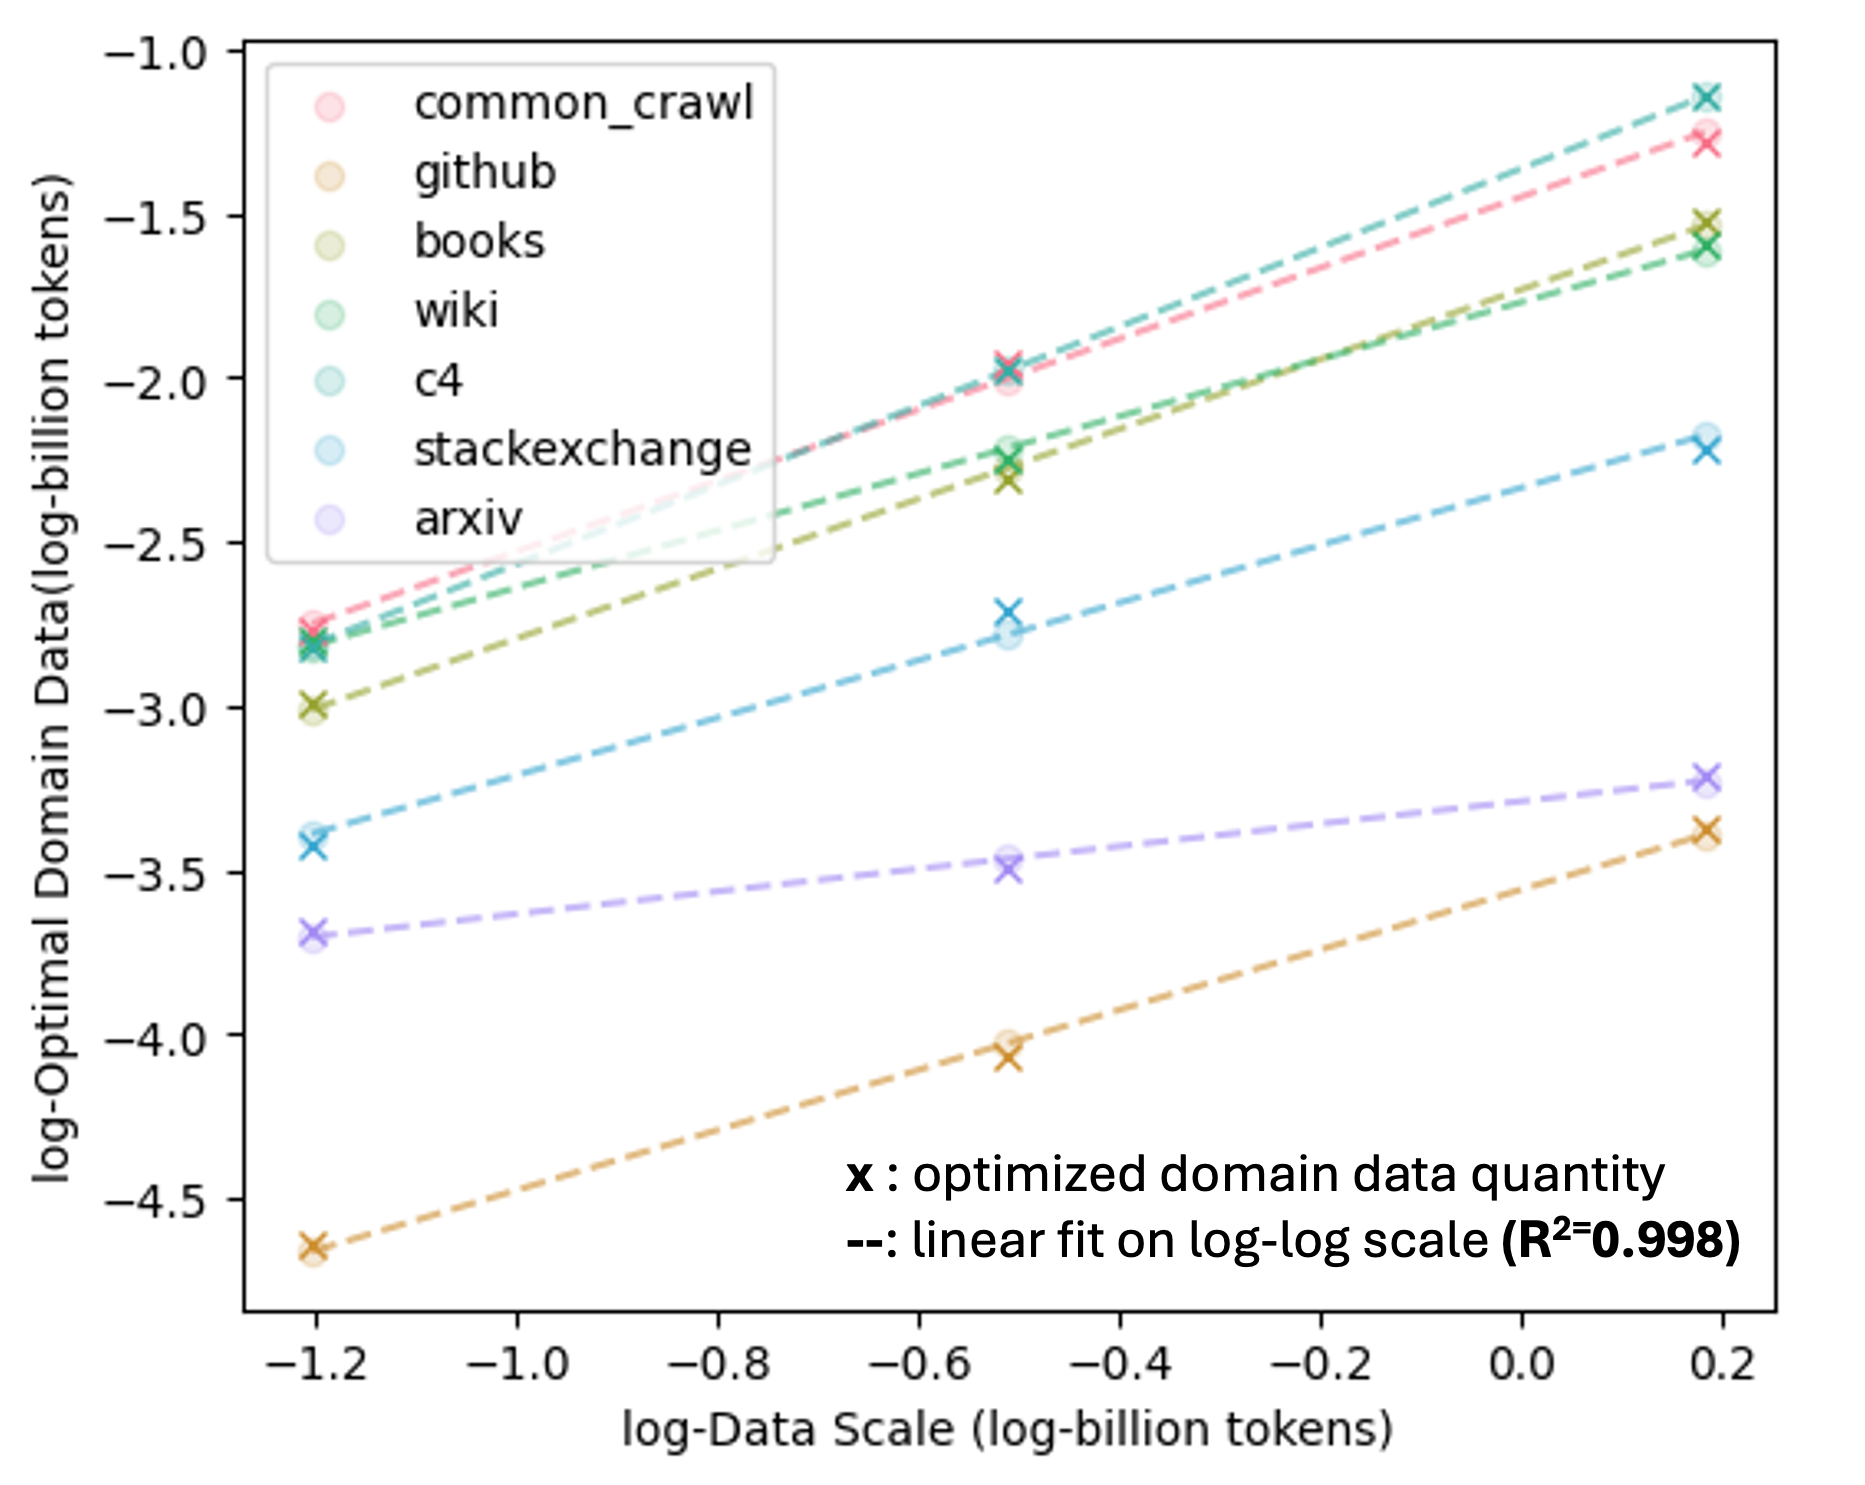
\includegraphics[width=0.7\textwidth]{figs/figfaithr2.png}
%   \vspace{-1em}
%   \caption{linear fit in log-log scale.
%   }\label{fig:example}
%   \vspace{-1em}
%   \end{center}
% \end{figure}% \vspace{-1em}




% \begin{figure}[h!]% \vspace{-1em}
%     \centering
%     \begin{subfigure}[b]{0.58\textwidth} % 0.59
%         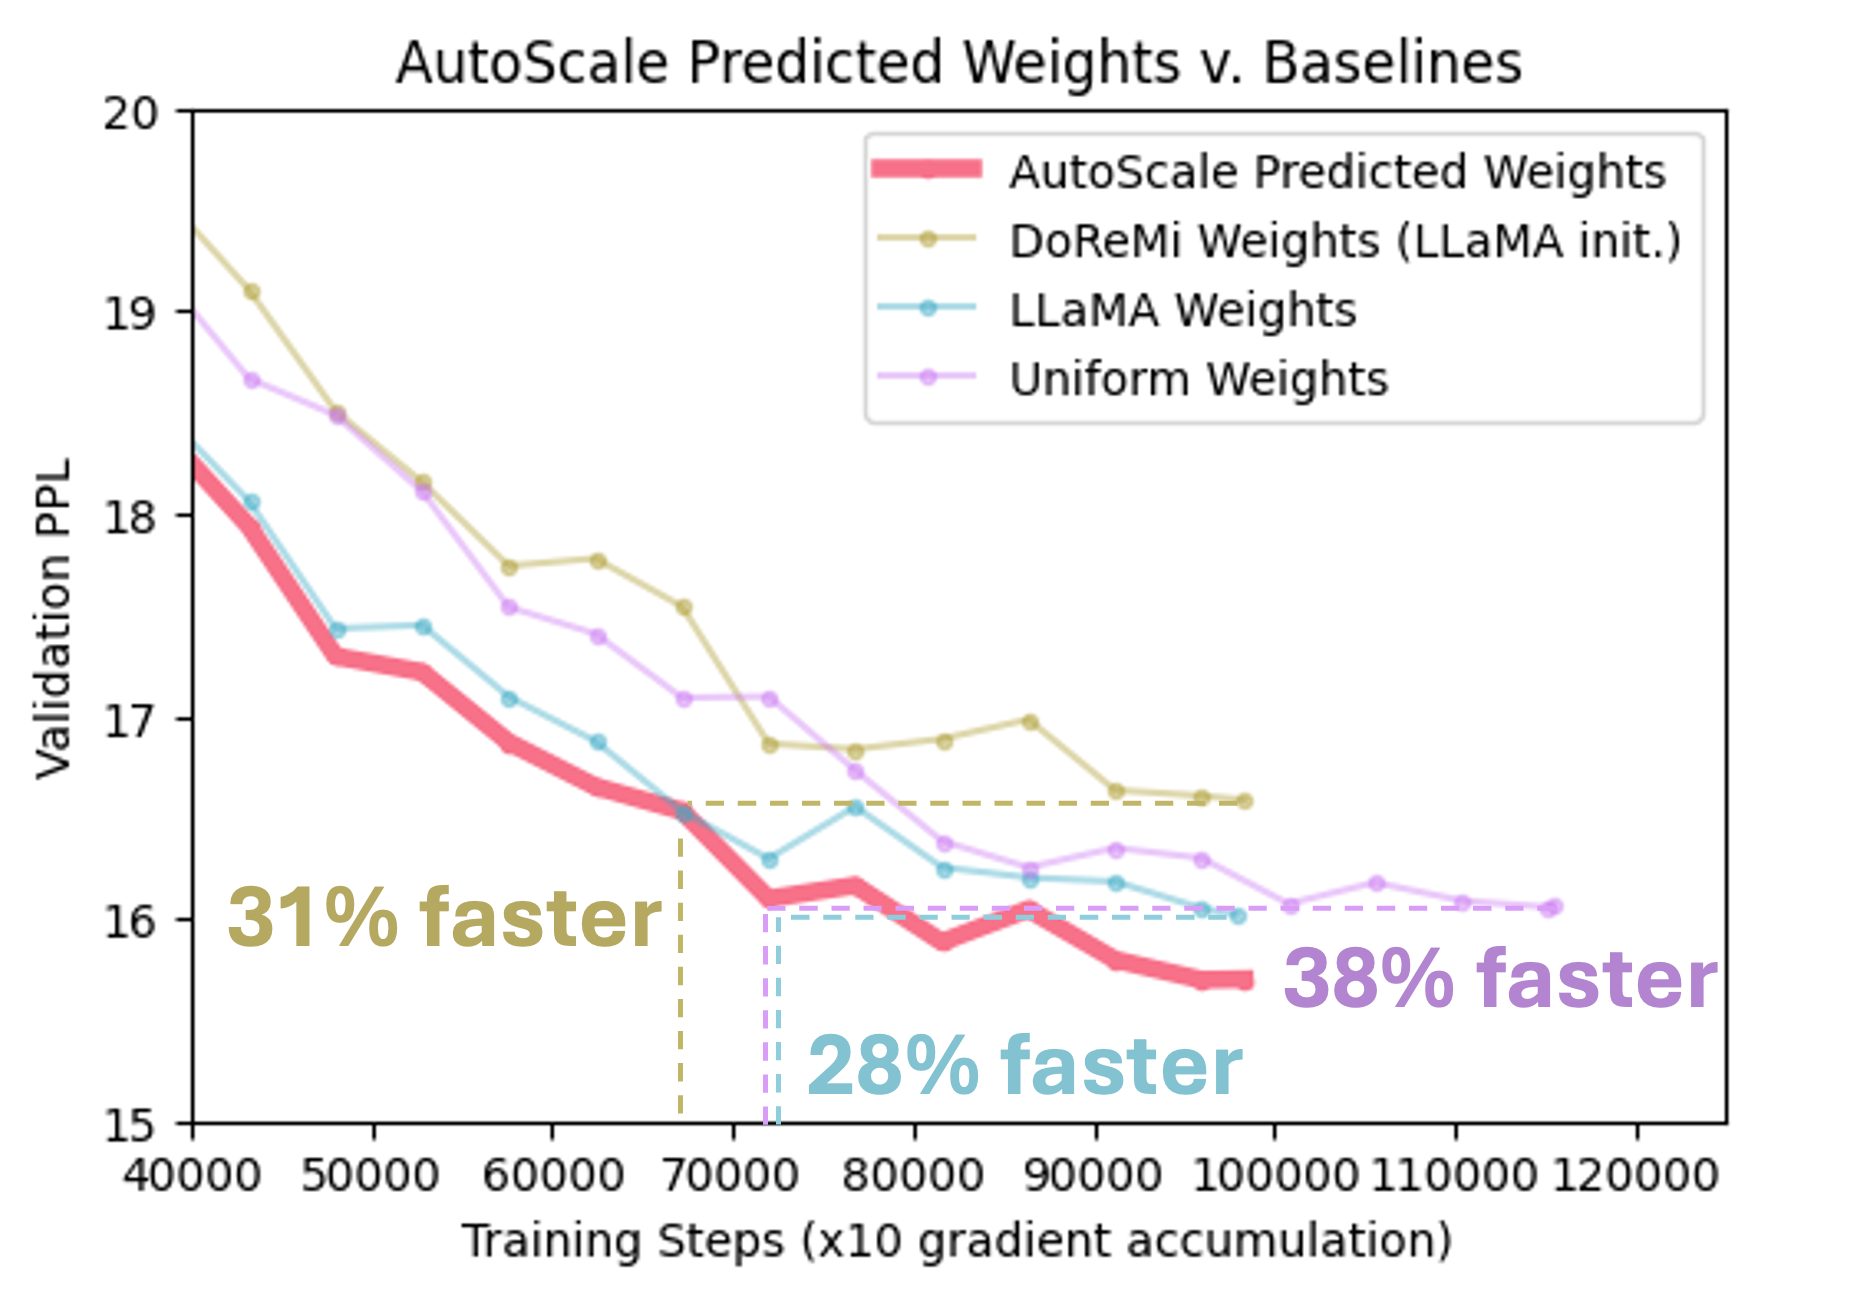
\includegraphics[width=\textwidth]{figs/fig1nline.png}\vspace{0.5em}
%         \caption{Validation Perplexity. ($\downarrow$ lower is better)}
%         \label{fig:figure8a}
%     \end{subfigure}
%     % \hfill
%     % \hspace{2em}
%     \begin{subfigure}[b]{0.39\textwidth} %0.345
    
%         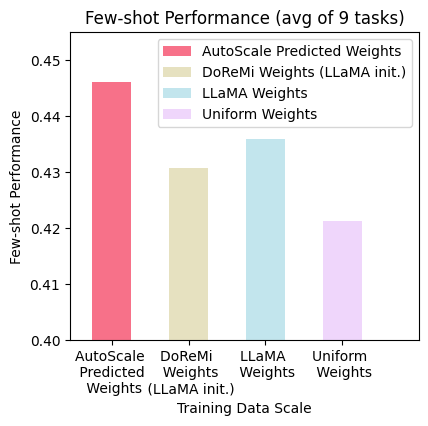
\includegraphics[width=\textwidth]{figs/fig2n3.png}\vspace{-0.5em}
%         \caption{Downstream Task Performance at 96k Steps. ($\uparrow$ higher is better)}
%         \label{fig:figure8b}
%     \end{subfigure}
%     \caption{Training 774M Decoder-only LMs for 10B tokens (96k steps). \textsc{AutoScale}-predicted domain weights decrease validation PPL at least $28\%$ faster than any baseline with up to $38\%$ speed up. LLaMA weights yield a much better training efficiency than uniform weights when scaling up.\rrm{I think Fig 2(a) is nice, but it should only be here if it is actually referenced and discussed in the Intro. I believe the other figures should go to the back where they are closer to the discussion.}}
%     \label{fig:figure8}% \vspace{-1em}
% \end{figure}


%Thus, the potential for improved training efficiency via principled domain reweighting remains unknown.



This work explicitly investigates and confirms the scale-dependence of optimal domain mixing, characterizing its scaling behavior. Based on these findings, we develop a practical methodology: optimizing domain weights at smaller, affordable scales and leveraging derived scaling laws to predict optimal mixing at much larger target scales. We lay out an overview of this work and main results in Fig. \ref{fig:example1}. Our contributions are summarized as follows.

\small{\circled{1}}\normalsize \textbf{ Principled algorithmic framework for optimal domain mixing.} Investigating the scaling law of domain mixing extends beyond mere empirical study. It requires a mathematical definition of optimal domain mixing and a tractable algorithm to solve for optimal weights. Our first contribution is formulating the optimal mixing problem as a bi-level optimization. However, existing general bi-level optimization techniques~\citep{colson2007overview,zhang2024introduction} are intractable in this context due to their reliance on second-order information. We propose a novel approach tailored to our problem context that leverages scaling laws to estimate the dependence of the learned model's loss on the weights, effectively reducing the bi-level problem to a single level. Our algorithm requires retraining models only linearly in the number of data domains, making it feasible for exploratory studies.

\small{\circled{2}}\normalsize \textbf{ Uncovering and quantifying the scale-dependence of optimal domain composition.\vspace{-0.3em}} \\
Leveraging the algorithm developed in \small{\circled{1}}\normalsize, we conduct empirical studies to optimize domain weights at different training data scales. Our results demonstrate that the optimal data composition varies with the scale of the training data, suggesting that the common practice of empirically determining an optimal composition using small-scale experiments will not yield optimal data mixtures for larger scales. We further derive an analytical framework for modeling the functional relationship between optimal data composition and training data scales.


\small{\circled{3}}\normalsize \textbf{ Practical algorithm for optimal domain mixing.} While the algorithm in \small{\circled{1}}\normalsize~has made optimal domain mixing feasible for exploratory studies, its retraining requirements limit its practicality to smaller scales. To enable data composition optimization at large scales, we propose \textsc{AutoScale}. This method works by finding optimal data compositions at smaller, computationally feasible scales, fitting a predictor using our analytical model for the scale-dependency of optimal composition mentioned in \small{\circled{2}}\normalsize, and finally using this predictor to determine optimal data composition at larger scales. Since one only needs to train models on small data scales where re-training is affordable, $\textsc{AutoScale}$ does not require using proxy models with a smaller parameter size, avoiding transferability issues between domain weights optimized with different model sizes.

\small{\circled{4}}\normalsize \textbf{ Robust performance gains across models and datasets.} Our evaluation of \textsc{AutoScale} on both decoder-only and encoder-only models demonstrates its consistent ability to achieve significant computational savings. For instance, in pre-training \texttt{GPT-2 Large} \citep{radford2019language} on the \texttt{RedPajama} dataset, \textsc{AutoScale} decreases validation perplexity 28\% faster than any baseline, with up to 38\% speed-up compared to training without reweighting. It also achieves the best overall performance across downstream tasks.
Additionally, we present intriguing findings regarding the varying benefits of traditionally perceived high-quality and low-quality data sources across different training scales. Specifically, we observe that data sources with standardized formats, such as \texttt{Wikipedia} and scientific papers---often regarded as high-quality---are most beneficial at smaller scales but exhibit sharp diminishing returns as the training data scales up. Conversely, with increased compute, data sources containing diverse examples, such as \texttt{CommonCrawl}, demonstrate continued reductions in training loss even at considerably large training data scales.

% In empirical studies with pre-training 774M Decoder-only LMs (\texttt{GPT-2 Large}\citep{radford2019language}) on \texttt{RedPajama} dataset, \textsc{AutoScale} decreases validation perplexity at least 25\% \rrm{25\% or 28\%?} faster than any baseline with up to 38\% speed up compared to without reweighting, achieving the best overall performance over downstream tasks. On pre-training Encoder-only LMs (\texttt{BERT} \citep{devlin2018bert}) with masked language modeling (MLM), compared to without reweighting, \textsc{DDO} decreases loss on all domains while visibly improving average task performance on \texttt{GLUE} benchmark \citep{wang2018glue} by 8.7\% and on large-scale QA dataset, \texttt{SQuAD} \citep{rajpurkar2016squad}, by 5.9\%, where \textsc{AutoScale} further speeds up training by up to 28\%. \kang{Or add a box to the findings?}\textbf{We found data sources with standard format such as \texttt{Wikipedia} and scientific papers, regarded as high quality, are most beneficial at smaller scales but observe sharp diminishing returns as the training data scales up. With more compute, data sources with diverse examples, such as \texttt{CommonCrawl}, demonstrate continued reductions in training loss even at considerably large training data scales.}


% To navigate through these challenges, this work pioneers a novel approach, proposing a generic domain reweighting methodology for LLM pre-training. \textbf{Our efforts are three-fold:} % \vspace{-0.5em}

% \rrm{I am not sure why this is bulleted? Each are basically their own paragraphs, so either we should trim to bullet-size content or just keep paragraphs without bullets.}

% \begin{itemize}[noitemsep, left=0pt]
    % \item 
    % First, we demonstrate \textit{optimal data compositions are scale-dependent and show a consistent shifting pattern with training data scales, suggesting predictability}. To this end, 
    % We first formalize the problem of finding compute-optimal data composition with domain reweighting as bi-level optimization. Due to its prohibitive computational complexity, current work \citep{xie2024doremi,fan2023doge,ye2024data,liu2024regmix} mostly employs heuristic methods to conduct this optimization, achieving varying results in different cases. We propose an original solution algorithm, \underline{D}irect \underline{D}ata \underline{O}ptimization (\textsc{DDO}), for determining a compute-optimal training data composition for a given data scale by estimating and optimizing over the neural scaling law of the data sources. Effectively reducing the bi-level problem to a single level, this approach allows finding the global optimum in a reasonable time and with high precision.

% Then,  with the \textsc{DDO} algorithm, for a fixed model training pipeline, we conducted empirical studies to optimize domain weights at different training data scales. Our results demonstrate that the \textit{optimal data composition for a fixed compute budget depends on the scale of the training data, suggesting that the common practice of empirically determining an optimal composition using small-scale experiments will not yield optimal data mixtures for larger models.}
% Foreshadowed by \citep{sorscher2022beyond, goyal2024science}, beyond-neural scaling law performance might be attained if one could find the best training dataset for each training data scale. This consistent pattern of shifts suggests \textit{predictability} in the relationship between optimal composition and training data scales. Via the lens of scaling laws, this work pioneers in deriving an analytical framework for modeling the functional relationship between optimal data composition and training data scales, laying out theoretical foundations that could be of independent interest.

    % \item 
    % Second, seminal work \citep{sorscher2022beyond} suggests the possibility of attaining beyond-neural scaling law performance if one could find the best training dataset for each training data scale. We observe a similar pattern in optimizing training data composition for LLMs (Fig.~\ref{fig:figure1}). \rrm{I don't see immediately how Fig. 3 shows that we observe a similar pattern of going beyond neural scaling laws.  Fig. 3 is giving numerical results, and I do not have enough understanding of the paper to be able to analyze them and draw conclusions right now. This is an example of where I think these figures are better served in \S4 where they are properly discussed.}\kang{shows that optimal composition is scale-dependent and shifts with scale; could achieve better than fixed scaling law if one could track the pattern of shift} 
%  We show that the shift in the optimal data composition with the scale of training complies with a simple function form and is empirically predictable. By fitting this pattern of shift at smaller scales, we are able to predict optimal data compositions at larger scales, automatically adjusting data composition for any training data scale and achieving beyond-neural scaling performance improvements on the target model. Correspondingly, we propose \textsc{AutoScale}, an automated tool that finds a compute-optimal data composition for training an LLM at the target scale. With optimal data compositions found at smaller scales, we fit the \textsc{AutoScale} predictor designed based on theoretical analysis with scaling laws and use it to determine optimal data composition at larger scales. Since one only needs to train models on small data scales where re-training is affordable, $\textsc{AutoScale}$ \textit{does not require using proxy models with a smaller parameter size, avoiding the transferability issue between domain weights optimized on different models}.
% \end{itemize}

% Finally, we propose \textsc{AutoScale}, an automated tool that finds a compute-optimal data composition for training an LLM at the target scale. With optimal data compositions found at smaller scales, we fit the \textsc{AutoScale} predictor designed based on theoretical analysis with scaling laws and use it to determine optimal data composition at larger scales. Since one only needs to train models on small data scales where re-training is affordable, $\textsc{AutoScale}$ \textit{does not require using proxy models with a smaller parameter size, avoiding the transferability issue between domain weights optimized on different models}.

\begin{figure}[h!]
\begin{center}
\vspace{-2.1em}
\centering
  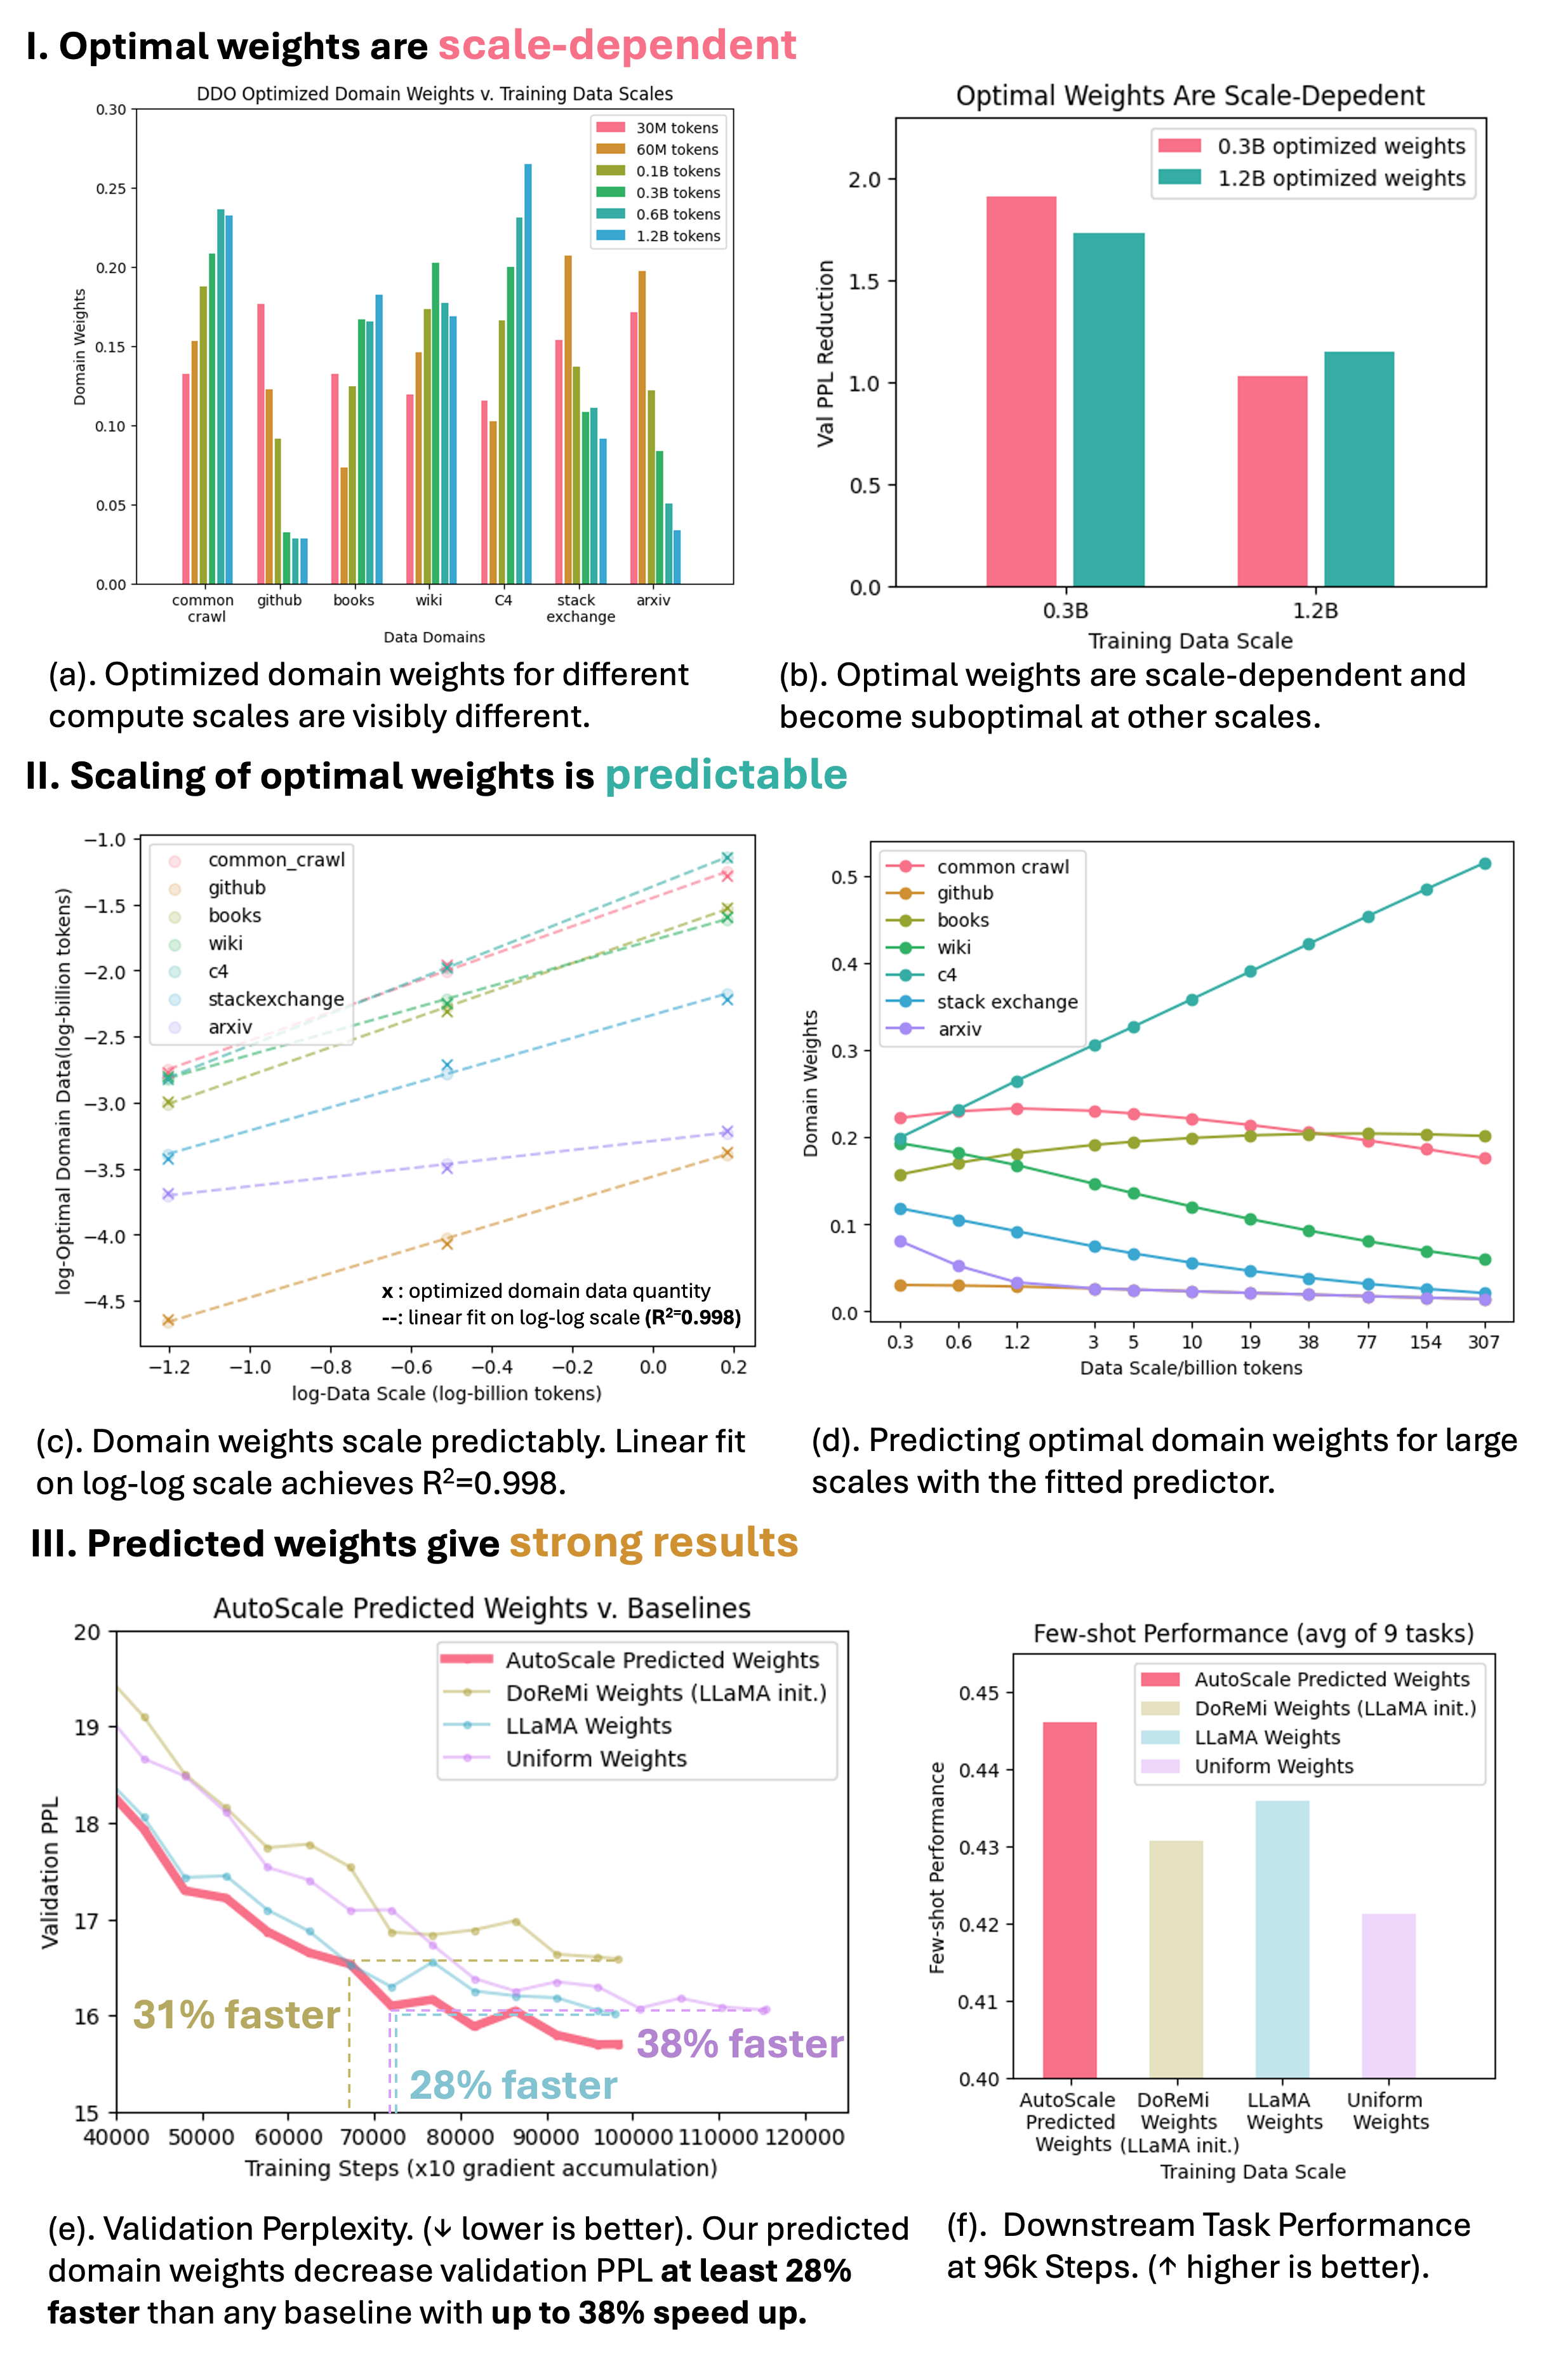
\includegraphics[width=.85\textwidth]{figs/agg4.png}
  \vspace{-0.5em}
  \caption{\small{Overview and main results. I. Optimizing domain weights with the proposed \underline{D}irect \underline{D}ata \underline{O}ptimization (\textsc{DDO}) algorithm for pre-training 774M Decoder-only LMs (\texttt{GPT-2 Large}). Optimal domain weights depend on the scale of training data. A consistent shift can be observed (\textit{data sources with standardized formats, such as \texttt{Wikipedia} and scientific papers---often regarded as high-quality---are most beneficial at smaller scales but exhibit sharp diminishing returns as the training data scales up. Conversely, with increased compute, data sources containing diverse examples, such as \texttt{CommonCrawl}, demonstrate continued reductions in training loss even at considerably large training data scales.}). Using domain weights optimized for a different scale yields sub-optimal results, failing to fully realize the benefits of domain reweighting. II. Optimal domain data quantity (y-axis) for different training data scales (x-axis) shows high linearity ($R^2=0.998$) on log-log plot, suggesting the shifting pattern can be well predicted by exponential-style functions. We fit \textsc{AutoScale} to predict optimal domain weights for larger training scales. As we scale up, data sources with diverse samples (e.g., \texttt{C4}) are upweighted relative to domains with standard format (e.g., \texttt{Wikipedia}). III. Training 774M Decoder-only LMs for 10B tokens (96k steps). \textsc{AutoScale}-predicted domain weights decrease validation PPL at least $28\%$ faster than any baseline with up to $38\%$ speed up, achieving best overall task performance. }\normalsize\vspace{-2em}
  }\label{fig:example1}
  \end{center}
\end{figure}% \vspace{-1em}


\vspace{-0.5em}
\section{Related Work}

\textbf{Domain Reweighting.} An emerging line of research strives to optimize the composition of training data for LLMs pre-training with \textit{domain reweighting} , i.e., adjusting the relative proportion of data from different data sources to "best" (in terms of training efficiency, final model performance, etc.) train the model. 
\textsc{DoReMi} \citep{xie2024doremi} first trains a small reference model, and then trains a second proxy model with GroupDRO \citep{sagawa2019distributionally} to minimize the excessive domain loss relative to the reference model, where the domain weights of the proxy model will be the output. \textsc{DOGE} \citep{fan2023doge} trains a proxy model while tracking the first-order gradient of the model on evaluation domains (i.e., data influence) and optimizes domain weights based on the gradients, relying on infinitesimal approximations which may or may not be accurate for models trained with a practical learning rate. \textsc{Data Mixing Laws} \citep{ye2024data} trains a number of proxy models to run a coarse grid search on the space of data mixtures and interpolate their performance with exponential functions to find the minimum. Similarly, \texttt{RegMix}\citep{liu2024regmix} trains a regression model to represent the relationship between training data mixtures and resulting model performance and optimize data composition based on it. 

These methods often rely on ad-hoc hyperparameter tuning via trial and error, achieving varying results. \textit{Further, the optimized weights are directly applied to training the target model on magnitudes of larger data scales.} This implicitly poses a strong assumption that the "optimal data composition" is invariant of model sizes or data scales. Yet, optimal data composition is likely to shift with data size. \textit{Optimal curation at a smaller scale may not remain optimal at the target scale} \citep{sorscher2022beyond,goyal2024science}. 
\citep{albalak2024survey} provides a recent survey for this fast-evolving field. We refer to App.~\ref{appendix_related_work} for broader discussions.   


\textbf{Scaling Laws.} Extensive research shows that \textit{Neural Scaling Laws}, predicting how the model performance changes with the scale of training data, model parameters, and computation budget \citep{kaplan2020scaling}, to be accurate in various tasks from vision and text processing \citep{ alabdulmohsin2022revisiting} to LLM pre-training \citep{rae2021scaling} and evaluations \citep{gadre2024language}. 
\citep{hoffmann2022training} proposes compute-optimal scaling for LLM pretraining data scales together with the model's parameter sizes. Yet, recent progress \citep{llama3modelcard,mehta2024openelm} shows no sign of saturation in pre-training even for models pre-trained on a considerably larger data scale than recommended by \citep{hoffmann2022training}. \citep{bahri2021explaining} shows that data from different sources generally scale at different rates. Seminal work \citep{sorscher2022beyond} sheds light on the possibility of attaining beyond-neural scaling law performance if one could find the best training dataset for each training data scale. This work is connected to the research on scaling laws in two ways. First, we leverage scaling laws to model the functional relationship between the quantity of data from each domain and trained model performance, allowing optimizing the training data composition in a reasonable time with high precision; further, \textit{this work contribute to a novel dimension of scaling laws–scaling optimal data compositions with the training data scale, providing original insights, clear empirical evidence, and theoretical frameworks which enable further analysis.}
% \textit{This work provides a novel perspective that leverages this dependency of scaling relationships with multiple data sources and at different data scales, predicting optimal data compositions at the target training data scale and achieving advantageous empirical results over scale-invariant training data mixtures.} 



% To overcome these limitations, our work makes two main contributions. First, we formalize the problem of finding compute-optimal data composition with domain reweighting as a bi-level optimization problem. We propose a meta-learning framework and a practical solution algorithm called Direct Data Optimization (DDO) to determine the optimal training data composition for a given data scale by estimating and optimizing over the neural scaling law of the data sources. This approach allows us to find the global optimum in a single step with high precision, achieving consistent results and reliable performance improvements across different use cases.

% Second, we observe that the optimal data composition shifts with the scale of training, and this shift follows a predictable pattern. By fitting this pattern at smaller scales, we can predict optimal data compositions at larger scales, automatically adjusting the data composition for any training data scale and achieving beyond-neural scaling performance improvements on the target model. We propose AutoScale, an automated tool that finds a compute-optimal data composition for training an LLM at the target scale by leveraging the optimal data compositions found at smaller scales and fitting them to a predictor designed based on theoretical analysis with scaling laws.

% Empirical studies on pre-training 774M Decoder-only LMs (GPT-2 Large) on the RedPajama dataset show that AutoScale decreases validation perplexity at least 25\% faster than any baseline, with up to 38\% speed up, achieving the best overall performance on downstream tasks. For pre-training Encoder-only LMs (BERT) with masked language modeling (MLM), DDO decreases loss on all domains while visibly improving average task performance on the GLUE benchmark by 8.7\% and on the large-scale QA dataset (SQuAD) by 5.9\%. AutoScale speeds up training by up to 28\%. Interestingly, we found that data sources with standard formats, such as Wikipedia and scientific papers, which are regarded as high quality, are only beneficial at smaller scales and exhibit sharp diminishing returns as the training data scales up. In contrast, data sources with diverse examples, such as CommonCrawl, continue to reduce training loss even at considerably large training data scales.

% \section*{Intro}
% Large language models (LLMs) are pre-trained using data from different sources or domains. Given the limited compute available for pre-training, it is necessary to determine an optimal composition of training data from these sources. 
% An emerging line of research strives to tackle this problem with  \textit{domain reweighting}, i.e., adjusting the relative proportion of data from different data sources \citep{xie2024doremi, chen2024skill, albalak2023efficient, soldaini2024dolma, fan2023doge, ye2024data}. Nonetheless, determining the optimal data composition is challenging. 

% Existing works often rely ad-hoc hyperparameter tuning via trial and error, yielding mixed results. \citep{wang2024survey} provides a recent survey for this fast-evolving field. [App.~A for extended related works] On the other end, recent progress repetitively shows pre-training LLMs on more data yields consistent benefits and predictably improves the model's utility and task performance with no sign of saturation [cite llama3 \citep{zhang2024tinyllama,mehta2024openelm}]. Scaling laws between the model's utility and the size of its training data are expected to continue in the foreseeable future. Due to the prominent costs and prevalent demand for larger-scale pre-training, a significant gap remains between current research progress and practical needs.  Data curation for LLM pre-training remains an open field with a strong call for contribution.

% There are crucial research questions for this problem where current investigations are limited.
% \begin{enumerate}[noitemsep, left=0pt]
%     \item \textbf{Understanding the potential of data curation and effectiveness of methods.} 
% Current methods for curating pre-training data often demonstrate unstable behavior or mixed results in practical implementations.  Some may be attributed to the experiment setups or methodology design. Industrial practice still relies on heuristic data curation \citep{mckinzie2024mm1}+[Apple]. Whether there is a good potential to substantially improve training efficiency/model performance via principled domain reweighting remains unknown. This renders it tricky to tell whether the adopted method is functioning or has failed, posing risks for practical adoption. [add citations]

% Existing methods for curating pre-training data often demonstrate limited efficacy or inconsistent behavior in practical implementations (e.g., underperforming random baselines at times). Some may be attributed to problematic method design (e.g., overly simple model/ungrounded approximations) or inappropriate experiment setups (e.g., false negative due to the signal being overwhelmed by noises). Industrial practice still relies on heuristic data curation (e.g., coarse grid scan on smaller scales then scale-up the best performing one.).  Whether there is a good potential to substantially improve training efficiency/model performance via principled domain reweighting remains unknown. More importantly, this renders it hard to tell whether the adopted method is functioning or have failed, posing risks for practical adoption.

% 2. \textbf{"SuperScaling", scaling of scaling laws}. 
% A majority of works aim to first optimize data composition for a smaller model and at a smaller data scale (i.e., proxy model) \citep{xie2024doremi,fan2023doge,ye2024data}. Then, the optimized weights are directly applied to training the target model on magnitudes larger data scales. This implicitly poses a strong assumption that the "optimal data composition" is invariant of model sizes or data scales. Yet, optimal data composition is likely to shift with data size. Optimal curation at a smaller scale may not remain optimal at the target scale \citep{goyal2024science}. This `meta-scaling' problem holds the promise to unlock more substantial performance improvements. [Fig. 1a] 
% \end{enumerate}

% A majority of current works aim to first optimize data composition for a smaller model and at a smaller data scale (i.e., proxy model/reference model) ([DOGE], [DoReMi], [Data Mixing Laws]). Then, the optimized weights are directly applied to training the target model on magnitudes larger data scales. This implicitly poses a strong assumption that the "optimal data composition" is invariant of model sizes or data scales. Yet, optimal data composition is likely to shift together with data size. Optimal curation at a smaller scale may not remain optimal at the target scale. [compute-aware] reveals that for multimodel foundation models (e.g., CLIP), optimal training samples are relative and dependent on the scale of the training dataset, where training samples that lead to the best performance at a smaller scale may become suboptimal if the training is conducted at a larger scale. Seminal work [beyond neural scaling] sheds light on the possibility of attaining beyond-neural scaling law performance if one could find the best training dataset for each training data scale. This 'meta-scaling' problem holds the promise to unlock more substantial performance improvements.

% This work strives to design and implement a generic data curation methodology for LLM pre-training that consistently achieve substantial performance improvements in practical scenarios. \textbf{Our efforts are two-fold.} 
% \begin{itemize}[noitemsep, left=0pt]
%     \item First, we formalize the problem of finding compute-optimal data composition with domain reweighting as bi-level optimization. This allows for directly optimizing the final objective over data composition, circumventing most of the risks from heuristic designs. Further, we propose a meta-learning framework and a practical solution algorithm, \underline{D}irect \underline{D}ata \underline{O}ptimization (\textsc{DDO}), for determining a compute-optimal training data composition for a given data scale by estimating and optimizing over the neural scaling law of the data sources. This provides a global approximation to this problem, which allows finding the global optimum in a \textit{single step} with high precision,  achieving consistent results and reliable performance improvements robust to different use cases [Fig. 2].

%     \item Second, seminal work [beyond neural scaling] suggests the possibility of attaining beyond-neural scaling law performance if one could find the best training dataset for each training data scale. We observe a similar pattern in optimizing training data composition for LLMs [Fig. 1b]. 
%     % In this work, we fill this gap by leveraging analysis via scaling laws. Our analysis reveals a novel result that the optimal data composition also scales with the training data size. This implies directly using domain weights optimized on proxy models or heuristically tuned for training other models will lead to suboptimal results or may not work at all. Further, 
%         We show that the shift in the optimal data composition with the scale of training complies to a simple function form and is empirically predictable. By fitting this pattern of shift at smaller scales, we are able to predict optimal data compositions at larger scales, automatically adjusting data composition for any training data scale and achieving beyond-neural scaling performance improvements on the target model. Correspondingly, we propose \textsc{AutoScale}, an automated tool that finds a compute-optimal data composition for training an LLM at the target scale. With optimal data compositions found at smaller scales, we fit the \textsc{AutoScale} predictor designed based on theoretical analysis with scaling laws and use it to determine optimal data composition at larger scales. 
% \end{itemize}


% \begin{figure}[h!]
%     \centering
%     \begin{subfigure}[b]{0.45\textwidth}
%         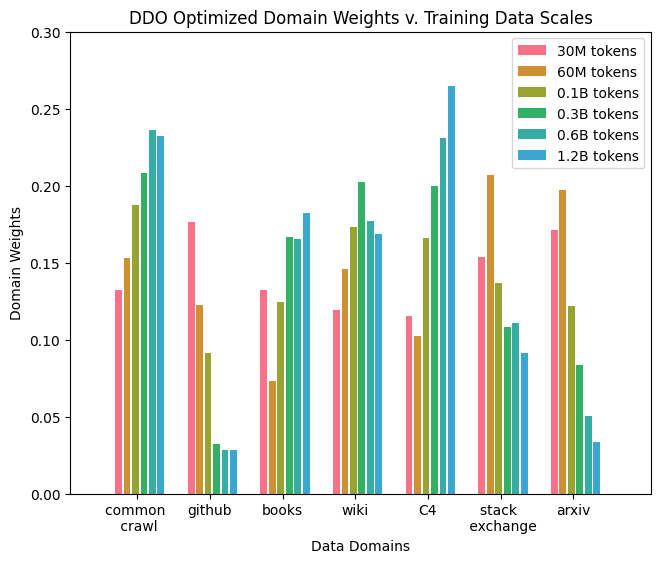
\includegraphics[width=\textwidth]{gptfigs/ddo5-200.png}
%         \caption{\textsc{DDO} Optimized Domain Weights}
%         \label{fig:figure1}
%     \end{subfigure}
%     % \hfill
%     \hspace{1em}
%     \begin{subfigure}[b]{0.45\textwidth}
%         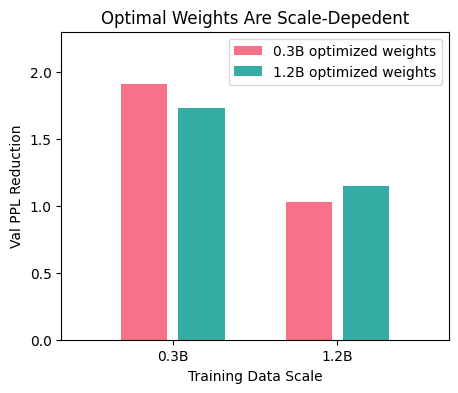
\includegraphics[width=\textwidth]{gptfigs/50-200cross.png}
%         \caption{Optimal Weights are scale-dependent}
%         \label{fig:figure2}
%     \end{subfigure}
%     \caption{GPT exps. Optimal domain weights are dependent on the scale of training data. A consistent shift can be observed. Using domain weights optimized for a different scale yields suboptimal results, not achieving the full potential of domain reweighting.}
%     \label{fig:figures}
% \end{figure}

% \begin{figure}[h!]
%     \centering
%     \begin{subfigure}[b]{0.48\textwidth}
%         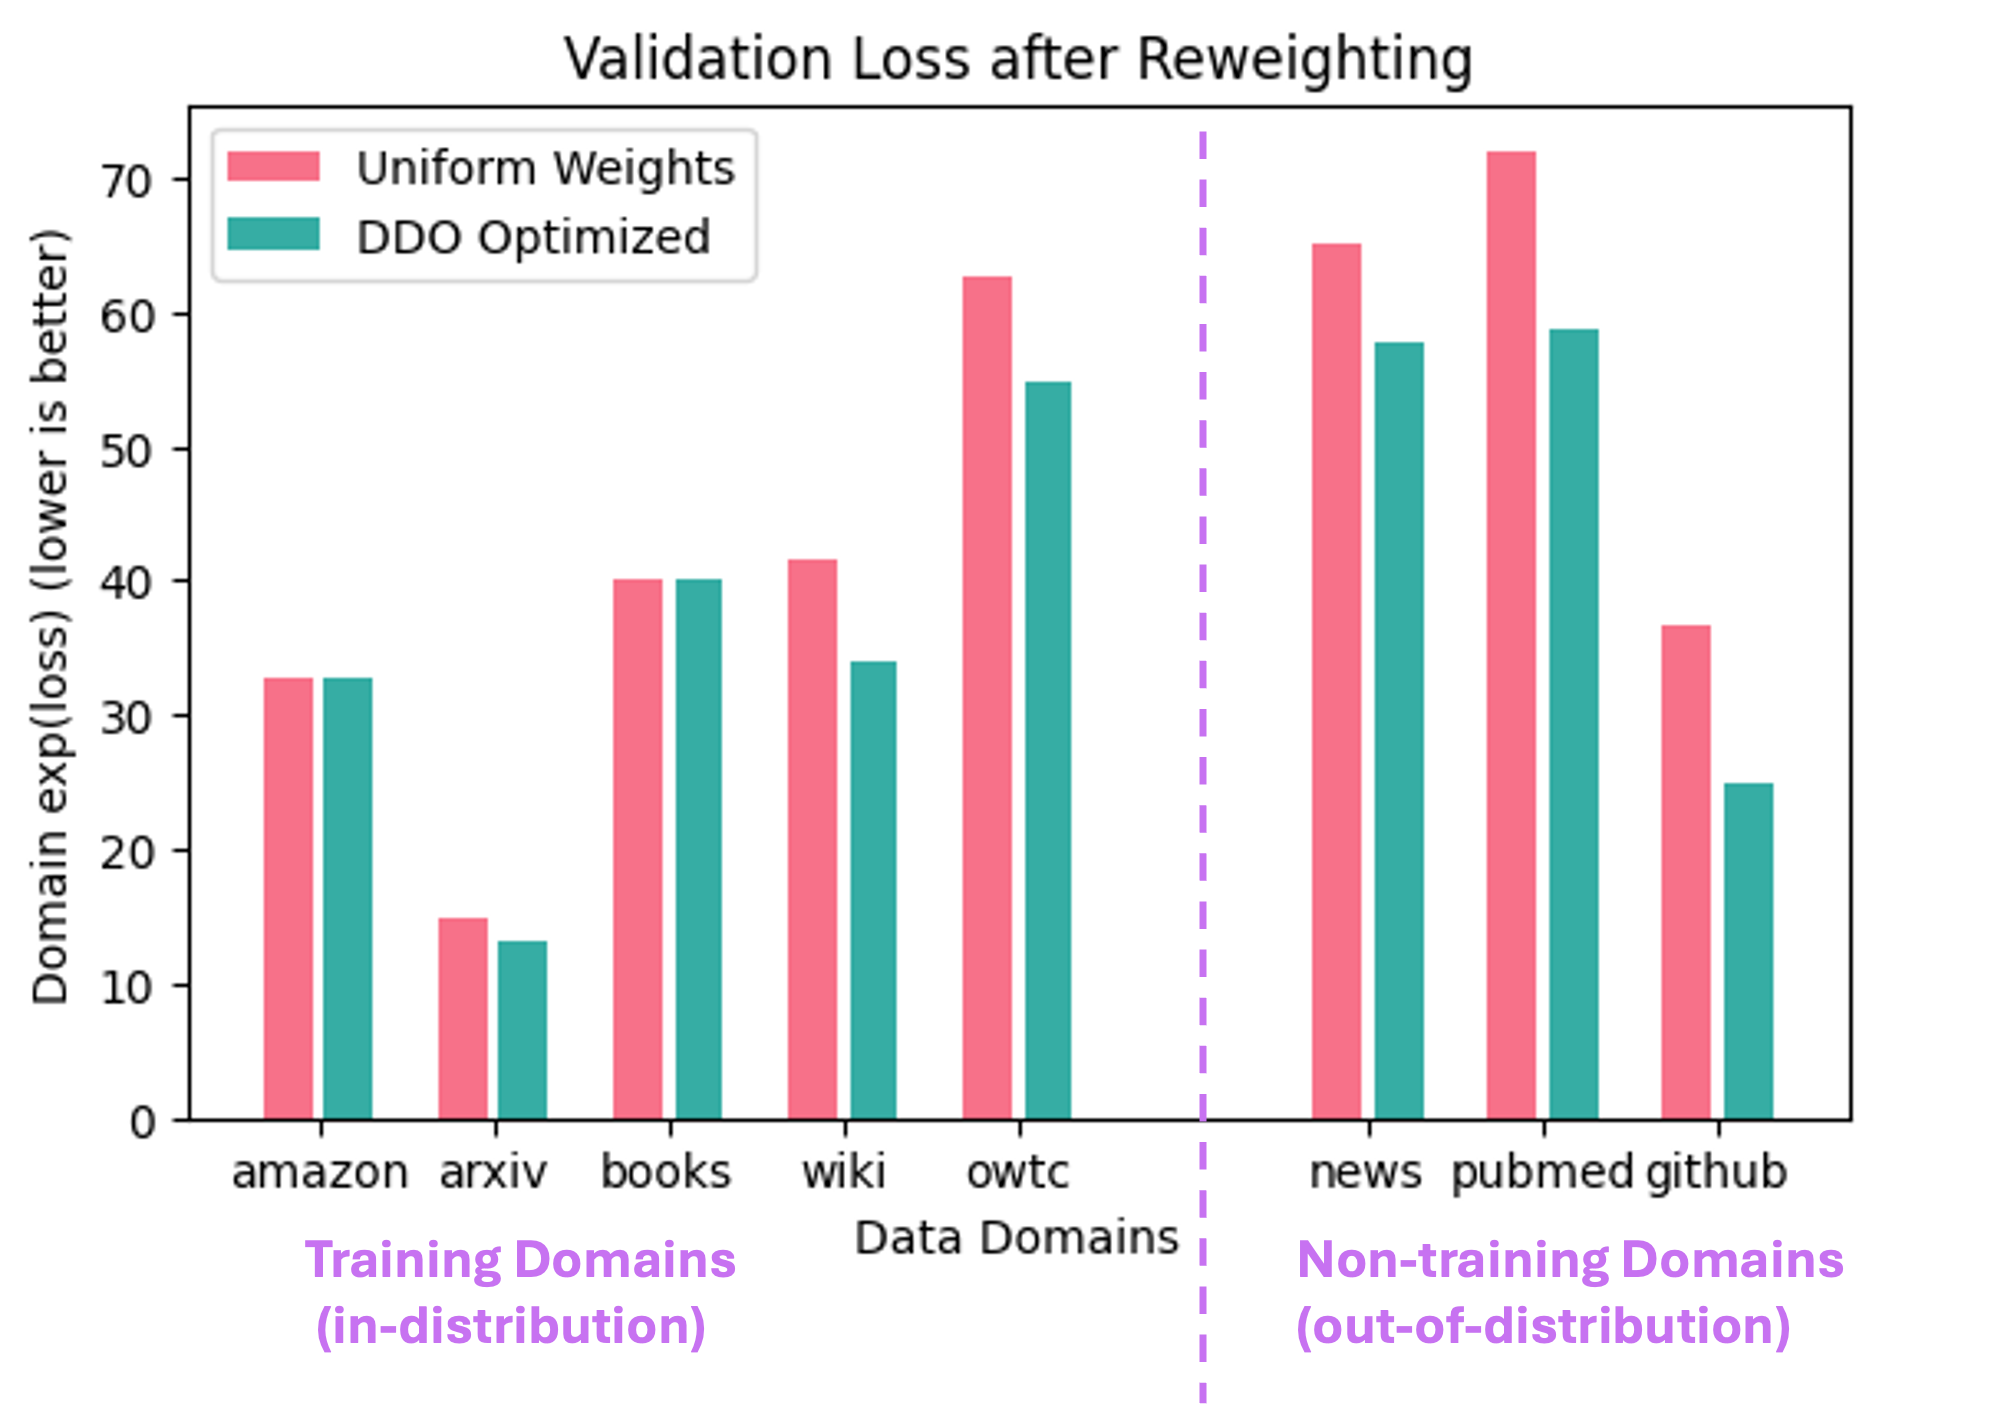
\includegraphics[width=\textwidth]{bertfigs/bert180pr.png}
%         \caption{Validation loss ($\downarrow$ lower is better)}
%         \label{fig:figure1}
%     \end{subfigure}
%     % \hfill
%     % \hspace{1em}
%     \begin{subfigure}[b]{0.48\textwidth}
%         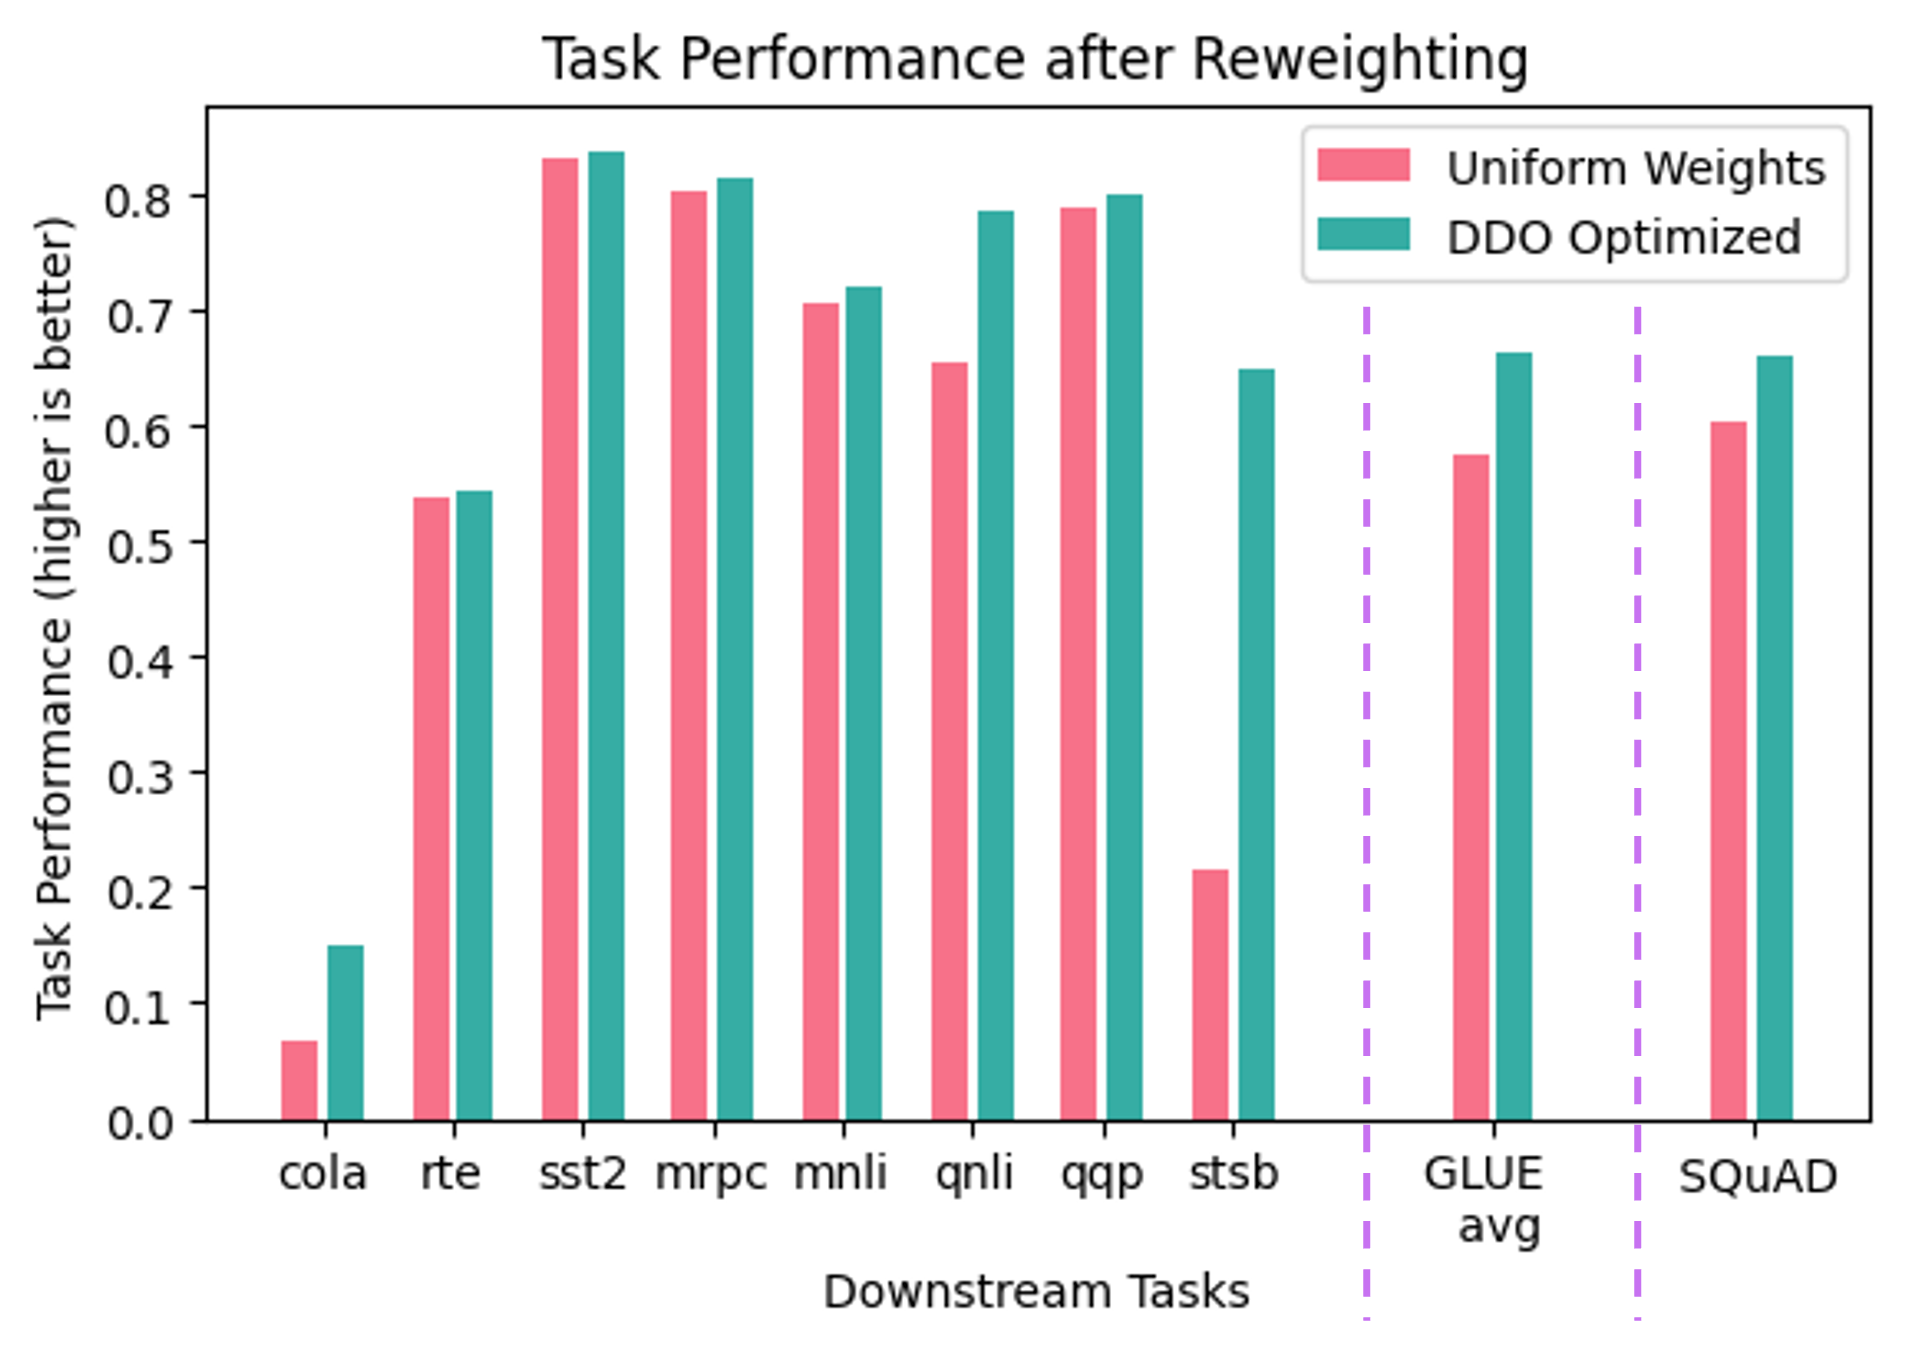
\includegraphics[width=\textwidth]{bertfigs/glue180pr.png}
%         \caption{Task Performance ($\uparrow$ higher is better)}
%         \label{fig:figure2}
%     \end{subfigure}
%     \caption{BERT \textsc{DDO}. \textsc{DDO} can substantially reduce average validation loss. In the case, after re-weighting training data, all domain's loss has either decreased or not changed. out-of-domain loss on held-out data also decreased considerably. better performance is achieved on all glue tasks and squad, a large-scale QA dataset.}
%     \label{fig:figures}
% \end{figure}

% In empirical studies with pre-training 774M Decoder-only LMs (\texttt{GPT-2 Large}) on \texttt{RedPajama} dataset, \textsc{AutoScale} decreases validation perplexity at least 25\% faster than any baseline with up to 38\% speed up, achieving the best overall performance over downstream tasks. On pre-training Encoder-only LMs (\texttt{BERT}) with masked language modeling (MLM), \textsc{DDO} is shown to decrease loss on all domains while visibly improving average task performance on GLUE benchmark by 8.7\% and on large-scale QA dataset (SQuAD) by 5.9\%. \textsc{AutoScale} speeds up training by up to 28\%.  We found data sources with standard format such as Wikipedia and scientific papers, regarded as high quality, are only beneficial at smaller scales and observe sharp diminishing returns as the training data scales up. With more compute, data sources with diverse examples, such as CommonCrawl, show to continue to reduce training loss even at considerably large training data scales. 

% In summary, this is the first work to directly solve for compute-optimal data composition via meta-learning or consider the scaling of scaling laws (“SuperScaling”) and shifts of optimal composition in LLM pre-training. This work sheds light on important patterns in this important problem and shall provide direct benefits to improve training efficiency and final model performance.  The proposed framework also lays the ground for developing curriculum learning schemes. Advancing the science of data curation for foundation models, together, these efforts will present a whole picture of this data problem and provide a concrete baseline for other works to evaluate upon.

% [workflow figure \kang{(is it needed?)}]

\vspace{-0.5em}
% \section{Compute-optimal Training Data Compositions}\vspace{-0.5em}
\section{Optimal Data Composition is Scale-Dependent and Predictable}\vspace{-0.5em}
\label{sec:ddo}
For "compute-optimal" domain weights, the goal is to find an optimal training data composition such that, for a given compute budget (i.e., training data size), the empirical validation loss, measured in perplexity (PPL), is minimized \citep{xie2024doremi,albalak2023efficient,fan2023doge}.  Formulating this as a bi-level optimization problem, in this section, we first introduce an original solution approach via scaling law approximations, which allows solving it efficiently and effectively. Then, with this solution approach, we solve for the optimal domain weights under different training data scales. Our results demonstrate that the optimal data composition for a fixed compute budget depends on the scale of the training data. Via the lens of scaling laws, this work pioneers in deriving an analytical framework for modeling the functional relationship between optimal data composition and training data scales.

\vspace{-0.5em}\subsection{Compute-Optimal Training Data Compositions}\vspace{-0.5em}




Consider training an LLM on a data composition $S$ from $m$ domains, $D_1, D_2, \cdots, D_m$. Let $S=\{S_1, S_2,\cdots, S_m\}$ denote the training dataset where $S_i$ is the subset of training data from each domain. The domain weights $\mathbf{w}=[w_1,w_2, \cdots, w_m]^T$ are defined as the proportions of data for each domain. Namely, letting $N=|S|$ denote the amount of total tokens of training data, domain weights are given as $w_i = N_i/N$, where $N_i$ denotes the amount of tokens for training subset $S_i$. % Let $S(N,\mathbf{w})$ denote the dataset of $N$ tokens composed from different domains using the weights $\mathbf{w}$. 

Let $\boldsymbol{\theta}^*(S)$ denote the parameters of a learning algorithm (i.e., the model) trained on data $S$ with empirical risk minimization (ERM), given as
% $
%     \theta^*={\arg\min}_\theta\mathcal{L}(\mathcal{A}(\theta),S)
% $
$
\boldsymbol{\theta}^*(S):= {\arg\min}_{\boldsymbol{\theta}}\mathcal{L}(\boldsymbol{\theta},S)
$
where $\mathcal{L}(\boldsymbol{\theta},S)$ denotes the loss of model parameterized by $\boldsymbol{\theta}$ evaluated on data $S$, which is the training loss. 
Since training data $S$ can be equivalently defined by 
its data quantity and domain weights $(N,\mathbf{w})$, we define a slight change of notation
$\boldsymbol{\theta}^*(N,\mathbf{w}) := \boldsymbol{\theta}^*(S)$ and will use $S$ and $(N,\mathbf{w})$ interchangeably.
% For simplicity, we use $\mathcal{A}(S)$ for the model $\mathcal{A}$ parameterized by $\theta^*$ trained with ERM on dataset $S$. 
We would like to maximize the amount of information gain and achieve maximum loss reduction during training, given as
$
        \min_{\mathbf{w}\in \mathbb{W}^m}\mathcal{L}(\boldsymbol{\theta}^*(N,\mathbf{w}), D^v) = \min_{\mathbf{w}\in \mathbb{W}^m}\sum_{i=1}^m \mathcal{L} (\boldsymbol{\theta}^*(N,\mathbf{w}), D_i^v)
$,
where $D^v$ and $D^v_i$ denote total validation data and validation data of individual domain $i$, respectively; the space of weights $\mathbb{W}^m$ is the hyperplane of the probability simplex
$
    \mathbb{W}^m=\{\mathbf{w}|w_1+w_2+\cdots+w_m=1\}\cap\{\mathbf{w}|0\leq w_i \leq 1, \forall i \in \{1,2,\cdots,m\}\}
$.
Define minor simplifications of notations for the validation losses
$\mathcal{L}^v(\theta, D^v) := \mathcal{L}(\theta, D^v)$ and $\mathcal{L}^v_i(\theta, D^v) := \mathcal{L}(\theta, D^v_i)$.
Then, the optimal domain weights, $\mathbf{w^*}$, are given as the minimizer of the objective,
\begin{align}
\label{eqn:upper}
   \mathbf{w^*}=\arg\min_{\mathbf{w}\in \mathbb{W}^m}\sum_{i=1}^m \mathcal{L}_i^v (\boldsymbol{\theta}^*(N,\mathbf{w})) \quad  \text{s.t.}\,\,\,\,\boldsymbol{\theta}^*(N,\mathbf{w}) = \arg\min_{\boldsymbol{\theta}}\mathcal{L}({\boldsymbol{\theta}},(N, \mathbf{w}))\vspace{-1.3em}
\end{align}
where perplexity is adopted as the loss metric.
This formulation is a bi-level optimization
problem, where the outer problem seeks the optimal domain weights, while the inner problem is training the model with ERM on the data defined by certain weights. A general approach is to solve it with gradient descent,
$
    \mathbf{w}^{t+1} = \mathbf{w}^{t} - \eta\cdot \frac{\partial \mathcal{L}_{v}(\boldsymbol{\theta}^*(N,\mathbf{w}^t))}{\partial \mathbf{w}}
$.
Since there is no tractable form of analytical expression for $\boldsymbol{\theta}^*$, this gradient needs to be estimated with empirical methods (e.g., approximated by finite difference), requiring repetitive re-training of the model at each update~\cite{liu2021investigating}. %It is worth noting that despite the rich literature on bi-level optimization~\cite{liu2021investigating}, traditional methods either rely on differentiating through the optimization process involved in the lower-level problem or require solving a linear system, which are not scalable for the setting of our interest. \rrm{This is seemingly dense and hard to follow.}

\subsubsection{Solution via Scaling-law-inspired Approximations}
% Optimizing training data composition via repetitive model retraining can be prohibitively expensive. Current work \citep{xie2024doremi,fan2023doge,ye2024data,liu2024regmix} mostly employs heuristic methods to conduct this optimization on smaller models trained with fewer data, achieving varying results in different cases. To crystalize the relationship between optimal data compositions and training data scales and obtain a clear image of the complete landscape, we propose an \textit{original} approach to this problem. With standard function approximations, this approach allows finding the global optimum in a reasonable time with high precision. 

Directly optimizing training data composition by solving bi-level optimization problems involves repetitive model retraining, which can be prohibitively expensive even at small scales. Current work \citep{xie2024doremi,fan2023doge,ye2024data,liu2024regmix} mostly employs heuristic methods to conduct this optimization 
on smaller models trained with fewer data, achieving varying results in different cases. To crystalize the relationship between optimal data compositions and training data scales and obtain a clear image of the complete landscape, we propose an \textit{original} approach to this problem.  We propose to first fit a scaling function to the outer loss (validation loss) $\mathcal{L}^v$ as a function of domain weights $\mathbf{w}$, effectively reducing the bi-level problem to a single level, which can be solved efficiently via regular gradient descent, allowing finding the global optimum efficiently and accurately.

%\rrmso{reduction in evaluation loss is maximized. For language models, the most commonly used evaluation metric is \textit{perplexity (PPL)}, defined as the exponentiation of cross-entropy loss.}{empirical validation loss, measured in perplexity (PPL), is minimized.} %In information theory, reduction in perplexity is considered to measure the amount of information gain. 
% \rrmso{Our objective is to maximize training efficiency by finding \textit{"compute-optimal"} domain weights for the training data. This setup has been adopted in this line of research \citep{xie2024doremi,albalak2023efficient,fan2023doge} and we will also follow in this work.}{We refer to this as determining "compute-optimal" domain weights corresponding to the different domains \citep{xie2024doremi,albalak2023efficient,fan2023doge}.} 




% \subsection{A Practical Solution via Meta-learning on Proxy Models–Direct Data Optimization (\textsc{DDO})}

% \vspace{-0.5em}\subsection{A Practical Solution via Scaling-law-inspired Approximation}\vspace{-0.5em}


% This formulation naturally produces a meta-learning problem, where our objective is the upper-level problem and the lower-level problem is training the model $\mathcal{A}$ on data $S$ defined by $(N,\mathbf{w})$. A general approach is to solve it numerically with gradient descent,
% \begin{equation*}
%     \mathbf{w}^{t+1} = \mathbf{w}^{t} - \gamma\cdot \frac{\partial \mathcal{L}^{P}_{v}(\mathcal{A}(N,\mathbf{w}^t))}{\partial \mathbf{w}}
% \end{equation*}
% Since there is no analytical expression for $\mathcal{A}$, this gradient needs to be estimated with empirical methods–e.g., approximated by finite difference, requiring repetitive re-training of the model at each update. 
% The standard practice is to optimize the data composition with \textit{proxy models} where re-training is plausible, and then optimized domain weights are used to train models at full-scale 
% [cite 1 2 3]. To achieve a practical algorithmic efficiency, instead, we provide a global approximation to this problem, which allows finding the global optimum in a \textit{single step} with high precision.

% [Data Mixing Laws] proposes to approximate the evaluation loss as a function of domain weights using a family of exponential functions.

% local approximation
% \begin{equation*}
%     \mathcal{L}^{P}_{v}(\mathcal{A}(N,\mathbf{w'})) - \mathcal{L}^{P}_{v}(\mathcal{A}(N,\mathbf{w^0})) =  \sum_{i=1}^m \left[a_i \cdot(N\cdot w_i')^{-\gamma_i}+\ell_i \right]
% \end{equation*}



\begin{wrapfigure}{R}{0.48\textwidth}\vspace{-1.4em}
\begin{minipage}{0.48\textwidth}
    \scalebox{0.48}{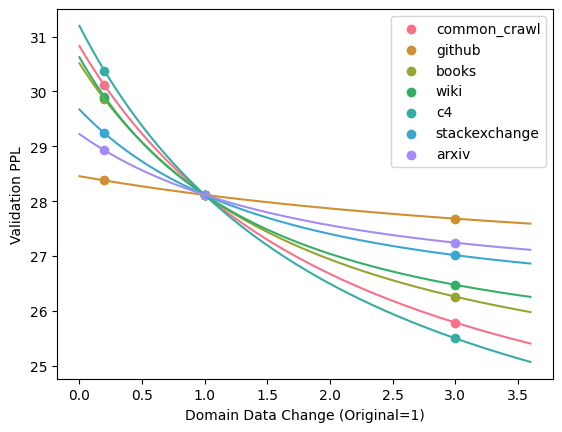
\includegraphics{gptfigs/gptddo.png}}\vspace{-0.2em}
    \caption{\small{Fitting validation loss with power-law functions for 774M Decoder-only LMs (\texttt{GPT-2 Large}), directly approximating how loss changes with each domain's data quantity. (\textit{X-axis depicts the quantity of domain data relative to the original amount before perturbation (e.g., 1.0=100\%).})}\normalsize}
    \label{fig:figure3}\vspace{-1em}
\end{minipage}
\end{wrapfigure}

% Inspired by neural scaling laws, we approximate the evaluation loss as a function of domain weights using a family of power functions,
To begin with, neural scaling laws suggest the relationship between a model's evaluation loss and the size of its training data can be well-represented by power law functions \citep{kaplan2020scaling}
$
    \mathcal{L}_{v}(\boldsymbol{\theta}^*(N,\mathbf{w})) =  N^{-\gamma}+\ell_0
$
where constants $\ell_0$ denotes some irreducible loss and $\gamma\geq 0$ is some scaling coefficient.
% \begin{equation*}
%     \mathcal{L}^{P}_{v}(\mathcal{A}(N,\mathbf{w})) =  \sum_{i=1}^m \left(a_i \cdot N_i^{-\gamma_i}+\ell_i \right)
% \end{equation*}
% where $N_i=|S_i|=N\cdot w_i$ denotes the amount of training data from domain $D_i$ and constants $a_i,\gamma_i,\ell_i$ are coefficients associated with each domain.
Drawing inspirations from \citep{hernandez2021scaling}, which formulates the scaling laws for transfer learning, we propose the following approximation to model the scaling relationship between model loss and training data quantity from different sources/domains.

Consider a model trained on data with size $N$ and domain weights $\mathbf{w}$. 
Define constant $N_0^i$ which estimates the evaluation loss when the amount of training data from domain $i$ is zero (i.e., $N_i'=0$), which effectively measures the effect of data from all other domains. From this regard, $N_0^i$ can be interpreted as the \textit{equivalent data size} for training data from domains other than $i$. Notably, this formulation aligns with empirical findings in the prior literature \citep{hernandez2021scaling,ye2024data}. Then,
for training data defined by $(N,\mathbf{w})$ where the amount of training data from \textit{domain} $D_i$ is $N_i=N\cdot w_i$, evaluation loss can be expressed as a  function of $N_i$:
$
        \mathcal{L}_{v}(\boldsymbol{\theta}^*(N,\mathbf{w})) = (N_0^i+N_i)^{-\gamma_i}+\ell_i 
$
where $\gamma_i,\ell_i$ are constants associated with domain $i$.
If the amount of training data from \textit{one domain} $D_i$ is changed from $N_i$ to $N_i'$ with the amount of training from other domains unchanged, we approximate the new model's evaluation loss, $\mathcal{L}_i'$, after re-training with a power law function of $N_i'$:
\begin{align}\vspace{-1.5em}
\label{eqn:scaling_law}
    \mathcal{L}_{v}(\boldsymbol{\theta}^*(N',\mathbf{w'})) = (N_0^i+N_i')^{-\gamma_i}+\ell_i :=\mathcal{L}_i'\vspace{-1em}
\end{align}
where $N'=N+(N_i'-N_i)$ denotes the updated amount of training data, and $w_i'=N_i'/N'$ denotes the updated domain weights. 

We propose the following procedure to fit the parameters in Eq. (\ref{eqn:scaling_law}). We re-train two models with different data quantities for domain $i$, $N_i^{+}$ and $N_i^{-}$ where $N_i^{-} < N_i<N_i^{+}$, and compute their evaluation loss, $\mathcal{L}_i^+$ and $\mathcal{L}_i^-$, respectively\footnote{Empirically, we found setting the perturbation ratio, $r=N_i/N_i^-=N_i^+/N_i=3$, produces reliable results.}. 
Then, together with evaluation loss $\mathcal{L}_v^0=\mathcal{L}_v(\boldsymbol{\theta}^*(N,\mathbf{w}))$ for the original model trained with $N_i$, the parameters $\gamma_i$, $\ell_i$ and $N_0^i$ can be estimated via ordinary least square (OLS) fitting, \vspace{-0.2em}
\small\begin{equation}
 N_0^i,\gamma_i,\ell_i = \arg\min_{N_0^i,\gamma_i,\ell_i} [\mathcal{L}_v^0-(N_0^i + N_i)^{-\gamma_i}-\ell_i]^2+[\mathcal{L}_i^+-(N_0^i + N_i^+)^{-\gamma_i}-\ell_i]^2+[\mathcal{L}_i^--(N_0^i + N_i^-)^{-\gamma_i}-\ell_i]^2
\end{equation}\normalsize
Compared to the original model, the difference in evaluation loss \textit{due to the change of data for domain $D_i$} is given as
$
    \mathcal{L}_{v}(\boldsymbol{\theta}^*(N',\mathbf{w'}))-\mathcal{L}_{v}(\boldsymbol{\theta}^*(N,\mathbf{w})) = (N_0^i+N_i')^{-\gamma_i} - (N_0^i+N_i)^{-\gamma_i}.
$
Repeating this process and fitting the scaling functions \textit{for each domain}, finally, we express the evaluation loss as a function of the amount of data from each domain as their summation:
$
    \mathcal{L}_{v}(\boldsymbol{\theta}^*(N',\mathbf{w'}))-\mathcal{L}_{v}(\boldsymbol{\theta}^*(N,\mathbf{w})) = \sum_{i=1}^m \left[ (N_0^i+N_i')^{-\gamma_i}- (N_0^i+N_i)^{-\gamma_i} \right]
$
where $N'=N+\sum_i(N_i'-N_i)$ and $w_i'=N_i'/N'$. \textit{Empirically, evaluation loss is shown to be well represented by such function form as depicted in Fig. (\ref{fig:figure3})}, which shows fitting validation loss with the proposed power-law functions for training 774M Decoder-only LMs (\texttt{GPT-2 Large}), directly approximating how loss changes with each domain’s data quantity. Results with Encoder-only LMs (\texttt{BERT}) demonstrates the same trend (Fig.~\ref{fig:figure30}(b)). This representation lends us an analytical form for the desired objective. 



% \rrm{Overall, I find this section to be very dense and moving very quickly. There is a lot of notation and rushing. One suggestion is to break this down into an enumerate where you outline high-level steps of what you are doing. Alternatively, consider slowing down through the steps, having more out-of-line equations and reducing notatino if possible.}

% This representation lends us an analytical form for the desired objective, which becomes\vspace{-0.5em}
% \begin{equation*}
%     \mathbf{w^*} =\arg\min_{\mathbf{w'}\in \mathbb{W}^m}\sum_{i=1}^m \left[ (N_0^i+N_i')^{-\gamma_i}- (N_0^i+N_i)^{-\gamma_i} \right] =\arg\min_{\mathbf{w'}\in \mathbb{W}^m}\sum_{i=1}^m (N_0^i+w_i'\cdot N')^{-\gamma_i}. 
% \end{equation*}

% \vspace{-1em}To derive the final objective from the middle one, we first note that $(N_0^i+N_i)^{-\gamma_i}$ is independent of $\mathbf{w}'$. Moreover, when we retrain model on the perturbed data sizes $N_i'$, we explicitly constrain the total amount of training data to be the same as before, i.e., $\sum_i N_i' = N$. Hence, $(N_0^i+N_i')^{-\gamma_i} = (N_0^i + w_i'\cdot N')^{-\gamma_i} = (N_0^i + w_i'\cdot N)^{-\gamma_i}$. 

% \vspace{-1em} Note that $(N_0^i+N_i)^{-\gamma_i}$ is independent of $\mathbf{w}'$, making it orthogonal to the optimization problem. 

To derive the final objective, we add the constraint for the total amount of training data to be the same as before, i.e., $\sum_i N_i' = N' = N$, which explicates our interest in reweighting data from each domain without changing the training data size. % Hence, $(N_0^i+N_i')^{-\gamma_i} = (N_0^i + w_i'\cdot N')^{-\gamma_i} = (N_0^i + w_i'\cdot N)^{-\gamma_i}$. 
Then, by definition, domain data quantity $N_i'=w_i'\cdot N'=w_i'\cdot N$.
Note that $(N_0^i+N_i)^{-\gamma_i}$ is independent of $\mathbf{w}'$, making it orthogonal to the optimization problem. Finally, our problem becomes
\vspace{-0.5em}\begin{equation*}
    \mathbf{w^*} =\arg\min_{\mathbf{w'}\in \mathbb{W}^m}\sum_{i=1}^m \left[ (N_0^i+N_i')^{-\gamma_i}- (N_0^i+N_i)^{-\gamma_i} \right] =\arg\min_{\mathbf{w'}\in \mathbb{W}^m}\sum_{i=1}^m (N_0^i+w_i'\cdot N)^{-\gamma_i}. \vspace{-0.5em}
\end{equation*}
% \ruoxi{$N$ in the final objective should be $N'$? if you delibrately perturb the data each domains in ways ensuring $N'=N$, we need explicitly menthion it; o.w., it's confusing}
% where $\sum_i N_i'=\sum_i N_i = N$. This optimization aims to minimize the new loss and maximize the loss reduction by adjusting the amount of training data from each domain. By the constraint on the total amount of training data same as before, its solution will re-weight the training data and find the optimal composition. 
Since the objective is defined as the summation of convex functions, we end up with a convex optimization problem. With the constraint on the probability simplex and the objective being easily differentiable, the problem can be solved extremely efficiently using \textit{projected gradient descent} \citep{bertsekas1997nonlinear}. We term this solution approach as \textsc{DDO} Algorithm (\underline{D}irect \underline{D}ata \underline{O}ptimization). We provide its pseudocode below and an operational pipeline in App.~\ref{app:operation}.

\begin{center}\vspace{-1.2em}
\scalebox{0.95}{\begin{minipage}{1.0\textwidth}
      \begin{algorithm}[H]
\caption{Direct Data Optimization (\textsc{DDO})}\label{alg:ddo}
\begin{algorithmic}
\Require $m$ domains (data sources) with data $D_1 \dots D_m$, data budget $N_0$ ($\ll$ for full-scale training), training dataset $S$, model parameters $\boldsymbol{\theta}$, validation loss $\mathcal{L}_v$, perturbation ratio $r>1$ (e.g., $r=3$).
\State Initialize weights for all domains $\forall i\in \{1,\dots m\}$: $w_i \gets 1/m$;
\State Initialize training data for all domains $\forall i\in \{1,\dots m\}$: sample $S_i \subset D_i$ where $|S_i|=w_i\cdot N$;
\State Train the model on data $S=\{S_1\dots S_m\}$ and evaluate its loss $\mathcal{L}_v^0 \gets \mathcal{L}_v(\boldsymbol{\theta}^*(S))$;
\For{$j$ from $1$ to $m$}
\State $w_j^+ \gets r\cdot w_j$; \Comment{Perturb domain weights (+)}
\State Resample $S_j^+ \subset D_j$ where $|S_j^+|=w_j^+\cdot N$;
\State Train the model on data $S=(\{S_1\dots S_m\}\setminus S_j)\cup S_j^+$ and evaluate its loss $\mathcal{L}_j^+ \gets \mathcal{L}_v(\boldsymbol{\theta}^*(S))$;
\State $w_j^- \gets \frac{1}{r}\cdot w_j$; \Comment{Perturb domain weights (-)}
\State Resample $S_j^- \subset D_j$ where $|S_j^-|=w_j^-\cdot N$;
\State Train the model on data $S=(\{S_1\dots S_m\}\setminus S_j)\cup S_j^-$ and evaluate its loss $\mathcal{L}_j^- \gets \mathcal{L}_v(\boldsymbol{\theta}^*(S))$;
\State OLS fit for scaling functions $N_0^i,\gamma_i,\ell_i = \arg\min_{N_0^i,\gamma_i,\ell_i} [\mathcal{L}_v^0-(N_0^i + N_i)^{-\gamma_i}-\ell_i]^2+[\mathcal{L}_i^+-(N_0^i + N_i^+)^{-\gamma_i}-\ell_i]^2+[\mathcal{L}_i^--(N_0^i + N_i^-)^{-\gamma_i}-\ell_i]^2$;
\EndFor
\State Output optimized domain weights $\mathbf{w^*} =\arg\min_{\mathbf{w'}\in \mathbb{W}^m}\sum_{i=1}^m (N_0^i + w_i'\cdot N)^{-\gamma_i}$.
\end{algorithmic}
% \rrm{This Algorithm block raises new questions, since there is now new notation introduced only in the Algorithm block, that wasn't there in the main text. What is the perturbation ratio $r$? Also $S^{-}_j$ is new notation. The part about perturbing domain  weights was also not really discussed in this section in the main text.}
\end{algorithm}\vspace{-1em}
\end{minipage}}
\end{center}
% convex since it is the simple summation of convex functions

% For $N>0$, since L0 is constant, we have
% \begin{equation*}
%     \begin{aligned}
%         \arg\min_{\mathbf{w}\in \mathbb{W}^m}\mathcal{L}^{P}_{v}(\mathcal{A}(N,\mathbf{w'})) =\arg\min_{\mathbf{w}\in \mathbb{W}^m}\sum_{i=1}^m \left[a_i \cdot (N_0^i+w_i'\cdot N)^{-\gamma_i}+\ell_i \right]
%     \end{aligned}
% \end{equation*}
% which gives
% \begin{equation*}
%     \begin{aligned}
%         \min_{\mathbf{w}\in \mathbb{W}^m}\sum_{i=1}^m a_i \cdot(N_0^i+w_i'\cdot N)^{-\gamma_i}
%     \end{aligned}
% \end{equation*}





\subsection{Optimal Data Compositions are Scale-Dependent}
With the \textsc{DDO} algorithm, for a fixed model training pipeline and data sources, we conducted empirical studies to optimize domain weights at different training data scales. Our results demonstrate that the optimal data composition for a fixed compute budget depends on the scale of the training data, suggesting that the common practice of empirically determining an optimal composition using small-scale experiments will not yield optimal data mixtures for larger models. 

Fig.~\ref{fig:example1}(a)(b) shows the results on 
optimizing domain weights with \textsc{DDO} algorithm for pre-training 774M Decoder-only LMs (\texttt{GPT-2 Large}). Optimal domain weights depend on the scale of training data. A consistent shift can be observed. Using domain weights optimized for a different scale yields sub-optimal results, failing to realize the benefits of domain reweighting fully. \textit{These results clearly show that the hypothesis, "optimal data composition is invariant of data scales", implicitly assumed by many existing works, is largely untrue.}
On the contrary, a consistent pattern can be observed in how optimal data compositions shift with the scale of training data. 
For example, data sources with standard format such as \texttt{Wikipedia} and scientific papers, regarded as high quality, are most beneficial at smaller scales but observe sharp diminishing returns as training data scales up. With more compute, data sources with diverse examples, such as \texttt{CommonCrawl}, demonstrate continued reductions in training loss even for larger training data scales.

Foreshadowed by \citep{sorscher2022beyond, goyal2024science}, beyond-neural scaling law performance might be attained if one could find the best training dataset for each training data scale. This treasure chest remains unexplored in the context of training LLMs. \textit{This consistent pattern of shifts suggests predictability in the relationship between optimal composition and training data scales}, holding the promise to unlock substantial improvements in training efficiency and model performance.





% \begin{figure}[h!]\vspace{-1em}
%     \centering
%     \begin{subfigure}[b]{0.45\textwidth}
%         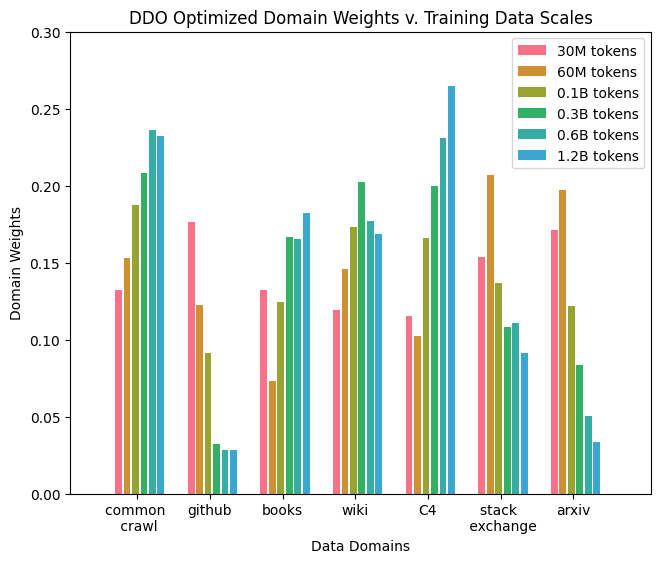
\includegraphics[width=\textwidth]{gptfigs/ddo5-200.png}
%         \caption{\textsc{DDO}-Optimized Domain Weights}
%         \label{fig:figure1a}
%     \end{subfigure}
%     % \hfill
%     \hspace{1em}
%     \begin{subfigure}[b]{0.45\textwidth}
%         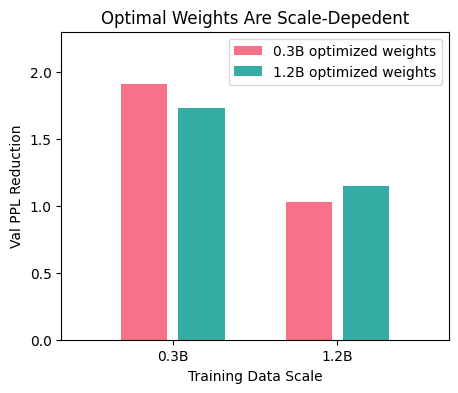
\includegraphics[width=\textwidth]{gptfigs/50-200cross.png}
%         \caption{Optimal Weights are Scale-dependent}
%         \label{fig:figure1b}% \vspace{-1em}
%     \end{subfigure}
%     \caption{Optimizing domain weights with \textsc{DDO} algorithm for pre-training 774M Decoder-only LMs (\texttt{GPT-2 Large}). Optimal domain weights are dependent on the scale of training data. A consistent shift can be observed. Using domain weights optimized for a different scale yields sub-optimal results, failing to fully realize the benefits of domain reweighting.\kang{will remove}}
%     \label{fig:figure1}
% \end{figure}


\subsection{Deriving Scaling Laws for Predicting Optimal Data Composition}\label{sec:33n}
Following the above findings, this work pioneers in deriving an analytical framework for modeling the functional relationship between optimal data composition and training data scales. Via the lens of scaling laws, the analysis lays out theoretical foundations that could be of independent interest.


Recall that neural scaling laws give the relationship between evaluation loss and training data quantity as
$
\mathcal{L} =  N^{-\gamma} + \ell_0 
$
where $\mathcal{L}$ is the evaluation loss (e.g., perplexity), $\ell_0$ denotes some irreducible loss, and $\gamma\geq 0$ are some constant. $(\ell_0, \gamma)$ can be fitted empirically.
% The standard formulation for neural scaling laws, a log-linear relationship in the log-log scale and a power law function in the original scale. Cross-entropy loss is considered as in the log scale. Perplexity, by definition, is the exponentiation of average cross-entropy loss, which we will describe with the power-law scaling function.
% \begin{equation*}
% \begin{aligned}
% \mathcal{L}& = \beta\cdot N^{-\gamma} + \mathcal{L}_0 
% \end{aligned}
% \end{equation*}
Without loss of generality, consider a standard case where the evaluation metric is aggregated loss over multiple independent tasks where each training sample will only contribute to a single task and the loss of each task only scales with the amount of training data contributing to this task as a power law function. Then, for a total of $m$ tasks, the aggregated evaluation loss scales as the following
$
\mathcal{L} =\ell_0+\sum_{i=1}^m \beta_i\cdot N_i^{-\gamma_i},
$
where $\ell_0$ denotes some irreducible loss, $N_i$ denotes the quantity of data contributing to task $i$ %\rrm{This is confusing because you previously mentioned that each training sample corresponds to a single task. Then, we should have $m$ training samples and $m$ tasks. Why is there $N_i$ data points corresponding to task $i$?}, 
and constants $\beta_i\geq 0$ and $\gamma_i\geq 0$ are coefficients associated with task $i$.
Define diagonal matrix $\mathbf{N}=diag\{N_1,N_2,\cdots N_m\}$.
For a training data scale $N=\sum_i N_i$, define compute-optimal data composition $\mathbf{N}=diag\{N_1^*, N_2^*,\cdots N_m^*\}$ as the minimizer of $\mathcal{L}$, given as
$
    \mathbf{N^*} = {\arg\min}_{\sum_i N_i=N} \ell_0+\sum_{i=1}^m \beta_i\cdot N_i^{-\gamma_i}
$.
We propose the following theorem, which states the optimal data composition scales in exponential-style functions with the amount of training data and can be directly predictable from that of smaller scales.

% \begin{theorem}
%  [Scaling Law for Optimal Data Compositions]
% \rrmso{For an evaluation loss that is aggregated over multiple independent tasks as described above,}{} if we have optimal data compositions $\mathbf{N^{(1)*}}=diag\{N_1^{(1)*}, N_2^{(1)*},\cdots N_m^{(1)*}\}$ which minimizes $\mathcal{L}$ s.t. $\sum_i N_i^{(1)*} = N^{(1)}$ and $\mathbf{N^{(2)*}}=diag\{N_1^{(2)*}, N_2^{(2)*},\cdots N_m^{(2)*}\}$ minimizes $\mathcal{L}$ s.t. $\sum_i N_i^{(2)*} = N^{(2)}$ where $N^{(1)}\neq N^{(2)}$, then optimal data compositions at other data scales $\mathbf{N^{(3)*}}=diag\{N_1^{(3)*}, N_2^{(3)*},\cdots N_m^{(3)*}\}$ which minimizes $\mathcal{L}$ s.t. $\sum_i N_i^{(3)*} = N^{(3)}$ where $N^{(3)} \neq N^{(2)}\neq N^{(1)}$ can be given as
% $
% \mathbf{N^{(3)*}} = \mathbf{N^{(2)*}}(\mathbf{N^{(1)*}})^{-1}\mathbf{N^{(2)*}}
% $.\label{thm}
% \end{theorem}
% \vspace{-0.5em}

% \rrm{I think this Theorem is written in a confusing nature. The result is not really about ML but is more of an optimization result. I have tried to rewrite the theorem in a way that is more clear. See below:}
\begin{theorem}\label{thm:thm1n}
    Consider the following optimization problem
    $
        \min_{\mathbf{N}} \left\{ \sum_{i=1}^m \beta_i N_i^{-\gamma_i} \Bigg| \sum_{i=1}^m N_i = N \right\}.
    $
    For any two compute budgets $N^{(1)} \neq N^{(2)}$, let $\mathbf{N}^{(1)*}$ and $\mathbf{N}^{(2)*}$ be their respective minimizers. 
    Then, there always exists some third data composition $ \mathbf{N}^{(3)*} = \mathbf{N}^{(2)*}(\mathbf{N}^{(1)*}) ^{-1} \mathbf{N}^{(2)*}$ such that $\mathbf{N}^{(3)*}$ is the minimizer for data budget $N^{(3)}=\sum_{i=1}^m N^{(3)}_i$, given as 
         $
        \mathbf{N}^{(3)*} = \arg\min_{\mathbf{N}} \left\{ \sum_{i=1}^m \beta_i N_i^{-\gamma_i} \Bigg| \sum_{i=1}^m N_i = N^{(3)} \right\}.
    $
    % Then, for any third compute budget $N^{(3)}$ such that $N^{(1)} \neq N^{(3)} \neq N^{(2)}$, the corresponding minimizer $\mathbf{N}^{(3)*}$ must satisfy $ \mathbf{N}^{(3)*} = \mathbf{N}^{(2)*}(\mathbf{N}^{(1)*}) ^{-1} \mathbf{N}^{(2)*}$.
\end{theorem}\vspace{-0.5em}


    See App.~\ref{app:lemma1} for the formal theorem statement and a complete proof. Examples for illustration are also provided in \ref{app:lemma1}. 
    We built our theory from a standardized example which assumes the evaluation metric is composed of independent tasks with separate scaling laws. In App.~\ref{app:theorem1}, we further extend this theory to a general case where the same conclusion can be reached without the independence assumption, where we consider the evaluation to be composed of a number of \textit{independent} sub-tasks (e.g., "latent skills" \citep{tiong2024toward}) which are hidden variables. Finally, we note that empirical results are shown to be highly consistent with the derivations above: In Fig.~\ref{fig:example1}(c), optimal domain data quantity (y-axis) for different training data scales (x-axis) shows high linearity ($R^2$ = 0.998) on log-log plot, \textit{suggesting the shifting pattern can be well-described by the exponential-style function forms described above.}

\vspace{-0.5em}
\section{\scalebox{0.96}[1.0]{\text{Towards A Practical Algorithm for Finding Optimal Compositions}}}
\label{sec:scaling}\vspace{-0.5em}
% \kang{much of it should be the introduction}
% Current methods for optimizing training data composition for LLMs are predominately compute-agnostic [cite 1 2 3 ]. The data composition is only optimized once, typically on a proxy model trained with much less data, and then the optimized weights are used for training the target model at full data scale. [DoReMi paper] shows the performance improvements from optimized domain weights are heavily dependent on the choice of proxy model (reference model), where using a 280M proxy/reference model yields the best domain weights for training the 8B target model while using either larger (1B) or smaller (70M/150M) proxy models are much less effective. [DOGE paper] shows that DoReMi produces very different results when the proxy model is trained on different amounts of data. Additionally, [DOGE paper] argues that the optimized domain weights are independent of parameter size for the proxy model, yet the results show a clear pattern where the optimized domain weights shift consistently with the size of the proxy model.

% [compute-aware] foreshadows that training data curation cannot be compute-agnostic. [compute-aware] reveals that for vision foundation model (e.g., CLIP), optimal training samples are relative and dependent on the scale of the training dataset, where training samples that lead to the best performance at a smaller scale may become suboptimal if the training is conducted at a larger scale. Seminal work [beyond neural scaling] sheds light on the possibility of attaining beyond-neural scaling law performance if one could find the best training dataset for each training data scale.

% We observe a similar pattern in optimizing training data composition for LLMs [add teaser results: data composition optimized for smaller scale are suboptimal at larger scales]. The benefit of data from different domains demonstrates a curriculum learning-like behavior with a clear pattern of phase transitions when the scale of training data becomes larger. For example, data sources with standard format such as Wikipedia and scientific papers, regarded as high quality, are more beneficial at smaller scales, but also saturate early and observe sharp diminishing returns as the training data scales up. With more compute, data sources with diverse examples, such as CommonCrawl, show to continue to reduce training loss even at considerably large training data scales.

% In this work, we intend to fill this gap by leveraging analysis via scaling laws. Our analysis reveals a novel result that the optimal data composition also scales with the training data size. This implies directly using domain weights optimized on proxy models or heuristically tuned for training other models will lead to suboptimal results or may not work at all. Further, we show that the shift in the optimal data composition with the scale of training complies to a simple function form and is empirically predictable. By fitting this pattern of shift at smaller scales, we are able to predict optimal data compositions at larger scales. This provides a viable approach for automatically adjusting data composition for any training data scale and achieving beyond-neural scaling performance improvements on the target model.

% \ruoxi{need to revise the introductory paragraph highlighting the connection between this section and the previous one. right now, 2 and 3 read a bit disconnected. E.g., While Sec.~2 provides an algorithmic framework to optimize the data composition at any scale, it is computationally expensive to directly perform optimization at a large target scale because it requires retraining models, which is only practical at a smaller scale. This section will investigate how to predict the optimal composition at a larger scale based on the composition optimized at smaller scales. In particular, we show that the optimal composition follows an exponential trend with respect to the scale, derived through a novel theoretical analysis and further justified through empirical observations.  }In this section, we first present a general theory that for an evaluation metric that is aggregated over multiple \textit{independent} tasks, the optimal composition of training data allocated to each task scales exponentially. Then, we extend the theory to illustrate how it generalizes to practical scenarios. We apply the theory to the case of maximizing perplexity reduction by optimizing the proportion of data from different domains and show that under general assumptions, the optimal composition of data from each domain scales exponentially with the training data scale.



\begin{wrapfigure}{R}{0.55\textwidth}\vspace{-1.75em}
    \scalebox{0.83}{\begin{minipage}{0.67\textwidth}
      \begin{algorithm}[H]
\caption{\textsc{AutoScale}}\label{alg:as}
\begin{algorithmic}
\Require Optimal domain weights (obtained from \textsc{DDO}) $\mathbf{w^{(1)*}}$at data scale $N^{(1)}$ and $\mathbf{w^{(2)*}}$ at data scale $N^{(2)}$, target data scale $N^{(t)}$, where $N^{(1)}<N^{(2)}<N^{(t)}$.

\State Optimal domain data $\mathbf{N^{(1)*}} \gets \mathbf{w^{(1)*}}\cdot N^{(1)}$;
\State Optimal domain data $\mathbf{N^{(2)*}} \gets \mathbf{w^{(2)*}}\cdot N^{(2)}$;
\State Next optimal domain data $\mathbf{N^{(x)*}} \gets \mathbf{N^{(2)*}}(\mathbf{N^{(1)*}})^{-1}\mathbf{N^{(2)*}}$;
\State Next data scale $N^{(x)} \gets \sum_i N_i^{(x)*}$;
\While{$N^{(x)} < N^{(t)}$}
\State Next optimal domain data $\mathbf{N^{(x)*}} \gets \mathbf{N^{(x)*}}(\mathbf{N^{(1)*}})^{-1}\mathbf{N^{(2)*}}$;
\State Next data scale $N^{(x)} \gets \sum_i N_i^{(x)*}$;
\EndWhile
\State Output predicted optimal domain weights $\mathbf{w^{(t)*}} \gets \mathbf{N^{(x)*}}/N^{(x)}$.
\end{algorithmic}
\end{algorithm}
    \end{minipage}}\vspace{-1em}
  \end{wrapfigure}


In this section, we introduce a practical paradigm for finding optimal data compositions developed based on the theoretical analyses and empirical insights introduced above. Having shown the consistent pattern of shifts in optimal data composition with the scale of training data and unveiled its predictability from scaling law analysis, moving forward, this paper presents a novel tool–$\textsc{AutoScale}$, which automatically predicts optimal training data compositions at larger scales based on compositions optimized at smaller scales. 

Theoretical analysis above shows that the optimal quantity for each domain scales in \textit{exponential-style functions} with training data size. 
We leverage this result to enable the automatic prediction of optimal training data compositions at larger scales from optimal compositions at small scales.
First, for two smaller training data scales $N^{(1)}$ and $N^{(2)}$ where $N^{(1)} \neq N^{(2)}$, find their optimal training data compositions $\mathbf{N^{(1)*}}$ and $\mathbf{N^{(2)}*}$ where $\sum_i N_i^{(1)*}=N^{(1)}$ and $\sum_i N_i^{(2)*}=N^{(2)}$ using \textsc{DDO} algorithm provided in Sec.~\ref{sec:ddo}. % Models trained at scales $N$ and $N'$ are considered proxy models where re-training these models is affordable. 

Since $N^{(1)}$ and $N^{(2)}$ are small data scales where re-training these models is affordable, $\textsc{AutoScale}$ \textit{does not require using proxy models with a smaller parameter size, avoiding the transferability issue between domain weights optimized on different models}.
Then, $\mathbf{N^{(1)*}}$ and $\mathbf{N^{(2)*}}$ yield the optimal training data composition at the next scale as
$
\mathbf{N^{(3)*}} = \mathbf{N^{(2)*}}(\mathbf{N^{(1)*}})^{-1}\mathbf{N^{(2)*}}
$,
where $N_i^{(3)*}=(N_i^{(2)*})^2/N_i^{(1)*}$ is the optimal amount of training data for each domain. This gives that for data scale $N^{(3)}=\sum_i N_i^{(3)*}$,
optimal domain weights are given as $w_i^{(3)*}=N_i^{(3)*}/N^{(3)}$. Then, $\mathbf{N^{(3)*}}$ can be combined with either $\mathbf{N^{(1)*}}$ or $\mathbf{N^{(2)*}}$ to make the next prediction. Repeat this process until the target training data scale is reached. The procedure is described in the pseudocode above with operational pipelines provided in App.~\ref{app:operation}.

% \textbf{Operational Pipeline (\textsc{AutoScale})}
% \begin{enumerate}\vspace{-0.5em}
% \item For two smaller training data scales $N^{(1)}$ and $N^{(2)}$ where re-training the model is affordable, find their corresponding optimal training data compositions $\mathbf{N^{(1)*}}$ and $\mathbf{N^{(2)*}}$ using \textsc{DDO} Algorithm described above;

% \item Predict the next optimal training data composition as $\mathbf{N^{(3)*}} = \mathbf{N^{(2)*}}(\mathbf{N^{(1)*}})^{-1}\mathbf{N^{(2)*}}$, yielding optimal domain weights $w_i^{(3)*}=N_i^{(3)*}/N^{(3)}$ at new training data scale $N^{(3)}=\sum_i N_i^{(3)*}$;
% \item Repeat this process until the target training data scale is reached.
% \end{enumerate}









% \begin{equation*}
% \begin{aligned}
% \mathbf{A}^{-1}\mathbf{N} &= \mathbf{K} \\
% \mathbf{A}^{-1}\mathbf{N'}(\mathbf{A}^{-1}\mathbf{N})^{-1} &= \mathbf{X} \\
% \mathbf{A}^{-1}\mathbf{N''}(\mathbf{A}^{-1}\mathbf{N}')^{-1} &= \mathbf{X}
% \end{aligned}
% \end{equation*}

% \begin{equation*}
% \begin{aligned}
% \mathbf{A}^{-1}\mathbf{N'}(\mathbf{A}^{-1}\mathbf{N})^{-1} &=
% \mathbf{A}^{-1}\mathbf{N''}(\mathbf{A}^{-1}\mathbf{N}')^{-1} \\
% \mathbf{N'}(\mathbf{A}^{-1}\mathbf{N})^{-1} &=
% \mathbf{N''}(\mathbf{A}^{-1}\mathbf{N}')^{-1} 
% \\
% \mathbf{N'}(\mathbf{A}^{-1}\mathbf{N})^{-1} &=
% \mathbf{N''}(\mathbf{A}^{-1}\mathbf{N}')^{-1} 
% \end{aligned}
% \end{equation*}

\vspace{-0.5em}
\section{Empirical Results}\vspace{-0.5em}
Two sets of empirical studies are conducted: Causal Language Modeling (CLM) in Sec.~\ref{sec:exp-gpt}, and Masked Language Modeling (MLM) in Sec.~\ref{sec:exp-bert}. We train models with up to 10B tokens and report the number of steps saved to reach the same evaluation loss (perplexity). We also report downstream task performance to benchmark performance improvements after training the same number of steps.



\subsection{Experimental setup}
% \call{@Yifan: help here.}


%\paragraph{Models and Datasets}


In Sec.~\ref{sec:exp-gpt}, we pretrain 774M Decoder-only LMs (\texttt{GPT-2 Large} architecture \citep{radford2019language}) \textbf{from scratch} on the \texttt{RedPajama} dataset \citep{together2023redpajama}. \texttt{RedPajama} dataset is an open-source reproduction of the training data used for LLaMA-1/2 models \citep{touvron2023llama}, totaling 1.2T tokens from 7 data domains with proportions: \texttt{Common Crawl} (67\%), \texttt{C4} \citep{raffel2020exploring} (15\%), \texttt{GitHub} (4.5\%), \texttt{Wikipedia} (4.5\%), \texttt{ArXiv} (2.5\%), and \texttt{StackExchange} (2.0\%). 
In Sec.~\ref{sec:exp-bert}, we pretrain 110M Encoder-only LMs (\texttt{BERT-base} architecture \citep{DBLP:journals/corr/abs-1810-04805}) \textbf{from scratch} on data from 5 typical sources—\texttt{Amazon Reviews}, \texttt{Arxiv}, \texttt{Books}, \texttt{Wikipedia}, and \texttt{Open WebText Corpus} \citep{Gokaslan2019OpenWeb}. Further details are in App.~\ref{sec:appendix_exp_details_gpt} and \ref{sec:appendix_exp_details_bert}. Runtime and GPU hours are documented in App.~\ref{runtime}.


% LLaMA
% RedPajama v1
% CommonCrawl, C4, wiki, books, arxiv, github, Stack Exchange

% GPT-2 Large
% 20 few-shot tasks

%---------------------------------------------------------------%


% Uniform, LLaMA weights (curated), DoReMi, Data Mixing Laws (ref) and DoReMi (ref)

% We compare the performance of our method with the domain weights proposed by DoReMi~\citep{xie2024doremi}. DoReMi presents a novel approach by optimizing domain weights using a proxy model to minimize the worst-case excess loss across different domains. DoReMi obtains domain weights through the training of two small scale auxiliary models. Initially, a reference model is well-trained utilizing reference domain weights. Subsequently, the proxy model is trained from scratch using GroupDRO optimization. Implementation details are available in App.~\ref{sec:appendix_baseline_details}.


\subsection{Causal Language Modeling with Decoder-only LMs (GPT)}
\label{sec:exp-gpt}

\textbf{Evaluation}
We test the perplexity on the held-out dataset, comprising 10K samples each from the 7 domains. For downstream tasks, we include: \texttt{BoolQ} \citep{clark2019boolq} (zero-shot), \texttt{HellaSwag} \citep{zellers2019hellaswag} (zero-shot, 10-shot), \texttt{PIQA} \citep{bisk2020piqa} (zero-shot), \texttt{TruthfulQA} \citep{lin2021truthfulqa} (zero-shot), \texttt{PubMedQA} \citep{jin2019pubmedqa} (10-shot), \texttt{CrowsPairs} \citep{nangia2020crows} (25-shot), and \texttt{ARC-Easy} \citep{clark2018think} (zero-shot). Additionally, \texttt{BBH Novel Concepts} \citep{srivastava2022beyond} task is added to the aggregated results for models trained beyond 10B tokens, making a total of 9 tasks. We select tasks that ensure the model's performance surpasses random guessing, spanning from question answering and commonsense inference to bias identification and scientific problem solving. These tasks provide a comprehensive assessment of model performance \citep{mehta2024openelm,gadre2024language}.
We adopt the evaluation framework from \citep{gao2021framework}.  More details are available in App.~\ref{sec:appendix_evaluation}.

\textbf{Baselines}
We report results for our methods (\textsc{DDO} and \textsc{AutoScale}) and 5 baselines–\textsc{Uniform}, \textsc{LLaMA weights} (curated), \textsc{DoReMi} (LLaMA weights initialization), \textsc{Data Mixing Laws from \citep{ye2024data}} and \textsc{DoReMi} from \citep{xie2024doremi} (uniform initialization). Uniform weights uniformly sample data from all domains, resulting in the same number of training tokens from each domain. LLaMA weights are a set of curated domain weights heuristically tuned for training LLaMA-1/2 models. We implemented \textsc{DoReMi} proposed in \citep{xie2024doremi}. \textsc{DoReMi} trains two smaller-scale auxiliary models (proxy models). First, a reference model is trained with the dataset's original domain weights, which are the LLaMA weights for \texttt{RedPajama} dataset. Then, optimized domain weights are obtained by using a proxy model to minimize the worst-case excess loss across different domains. We train both auxiliary models for 50K steps. Implementation details are available in App.~\ref{sec:appendix_baseline_details}. Besides, we compare with 2 domain weights from existing literature, which are optimized on the same dataset, \texttt{RedPajama}, with similar Decoder-only LMs. \textsc{Data Mixing Laws} \citep{ye2024data} first performs a grid search on the space of possible data mixtures and records evaluation loss for proxy models trained on these mixtures. Then, the loss is interpolated with exponential functions to find the optimal domain weights for the proxy model. \textsc{DOGE} \citep{fan2023doge} also implements \textsc{DoReMi} \citep{xie2024doremi} with auxiliary models trained for 50K steps but with the reference model trained with uniform weights. We evaluate the model trained on these domain weights to present a complete landscape.

% \kang{yifan: add this}
% We select tasks
% that achieves performance above random guess

% LM Evaluation Harness

\textbf{Direct Data Optimization (\textsc{DDO}):}
We conduct \textsc{DDO} Algorithm to optimize domain weights for models (774M Decoder-only LMs) trained from scratch with 30M to 1.2B tokens.
\textit{As depicted in Fig.~\ref{fig:example1}(a), optimal domain weights for each training data scale are visibly different and demonstrate a clear shifting pattern}. We found data sources with standard format such as \texttt{Wikipedia} and scientific papers, regarded as high quality, are most beneficial at smaller scales and observe sharp diminishing returns as the training data scales up. With more compute, data sources with diverse examples, such as \texttt{CommonCrawl}, continue to reduce training loss for even larger training data scales. 
In Fig.~\ref{fig:example1}(b), we validated this observation in Fig.~\ref{fig:example1}(b), where we trained two models with 0.3B tokens with domain weights optimized at 0.3B tokens and 1.2B tokens, and two models with 1.2B tokens with these weights, respectively. \textit{\textcolor{teal}{Takeaway 1: the results show that, the optimal weights are only optimal at the scale it is optimized and become suboptimal when applied on other scales.}}



\textbf{Predicting Optimal Weights at Larger Scales with \textsc{AutoScale}:}
With \textsc{DDO}-optimized weights from models trained up to 0.6B tokens, we fit \textsc{AutoScale} predictor and use it to visualize how the optimal domain weights will shift as we continue scaling up training data.
Depicted in Fig.~\ref{fig:example1}(d) and Fig.~\ref{fig:figure4}, as the training data scale grows, data sources with diverse examples, such as \texttt{C4} and \texttt{CommonCrawl}, will take up a considerable proportion of training data. Therefore, we expect LLaMA weights will perform better when the training data scale is sufficiently large. The results also suggest training on data from \texttt{Books} domain will continue to provide benefits. \textcolor{teal}{\textit{Takeaway 2: thus, }\textsc{AutoScale}\textit{-predicted domain weights give a larger weight to Books domain compared to baselines which counterintuitively downweight high-quality book contents}.}



\begin{table}[h!]
\centering\vspace{-0em}
\resizebox{\linewidth}{!}{
\begin{tabular}{l|ccccccccc}
\toprule
\textbf{Method/Task}                                                           & truthfulqa & pubmedqa       & piqa            & hellaswag       & crows\_pairs & boolq           & arc\_easy       & hellaswag  & \textbf{Avg}  \\
&\_mc2&&&(10-shot)&\_english&&&(zero-shot)&\\\midrule
Uniform Weights                                                               & 0.4526          & 0.438          & 0.6115          & 0.2923          & 0.5886                & 0.5636          & 0.3742          & 0.2907                & 0.4514         \\
LLaMA Weights                                                                 & 0.434           & 0.492          & 0.6055          & 0.2944          & \textbf{0.5903}       & 0.5612          & 0.3956          & 0.2952                & 0.4585          \\
\textbf{AutoScale (ours)}             & 0.4385          & \textbf{0.536} & \textbf{0.6202} & \textbf{0.3021} & 0.585                 & 0.6141 & \textbf{0.3977} & \textbf{0.303}        & \textbf{0.4746} \\
Data Mixing Laws (ref)                                                    & \textbf{0.4537} & 0.468          & 0.6061          & 0.2951          & 0.5778                & \textbf{0.6162}          & 0.3771          & 0.2938                & 0.4610         \\ 
DoReMi (ref)                                                    & 0.4505 & 0.468          & 0.5985          & 0.2886          & 0.5742                & 0.5410          & 0.3750          & 0.2896                & 0.4482         \\\bottomrule
\end{tabular}}\caption{Downstream task performance for 774M Decoder-only LMs trained for 3B tokens. Models trained with \textsc{AutoScale}-predicted weights achieve the best overall performance across the tasks.}\label{tab:gpt2_additional_2}
\end{table}

Subsequently, to examine \textsc{AutoScale}-predicted weights, we train models on larger scales with 3B, 5B, and 10B tokens. 
On 3B training data, we compare \textsc{AutoScale}-predicted weights with Uniform weights, LLaMA weights, \textsc{DoReMi} weights from \citep{fan2023doge} (uniform initialization), and \textsc{Data Mixing Laws} weights from \citep{ye2024data}. In both 3B and 5B results (Fig.~\ref{fig:gpt2_additional_3}), \textsc{AutoScale} \textit{achieves the lowest validation perplexity after the same steps, at least $25\%$ faster than any baseline with up to $37\%$ speed up}. Provided in Table \ref{tab:gpt2_additional_1}, \textsc{AutoScale}-predicted weights significantly reduced the loss on \texttt{Books} domain and also achieved much lowered worst-domain perplexity. When testing the few-shot performance on 8 downstream tasks, the model trained with \textsc{AutoScale}-predicted weights achieves the best overall performance (Table \ref{tab:gpt2_additional_2}).
Results for models trained with 10B tokens are depicted in Fig.~\ref{fig:example1}(e)(f), where we added the comparison with \textsc{DoReMi} initialized with LLaMA weights. \textcolor{teal}{\textit{Takeaway 3: }\textsc{AutoScale}\textit{-predicted weights consistently outperform any baseline with a $28\%$ to $38\%$ margin and demonstrate advantageous performance on downstream tasks. }} Echoing our predictions, as training data scales up, LLaMA weights visibly outperform uniform domain weights. See App.~\ref{sec:appendix_additional_results_gpt} for additional results .





\subsection{Masked Language Modeling with Encoder-only LMs (BERT)}
\label{sec:exp-bert}
We evaluate the model's MLM loss on held-out validation datasets, comprising 10K samples each from the 5 training domains. Additionally, as an auxiliary evaluation, we test the MLM loss on 3 non-training held-out domains. To be consistent with the perplexity loss used in CLM, we report the exponential cross-entropy loss for MLM. We evaluate the model's task performance on \texttt{GLUE} benchmark \citep{wang2018glue} (with 8 diverse tasks for natural language understanding (NLU)) and \texttt{SQuAD} \citep{rajpurkar2016squad} (a large-scale QA dataset). See App.~\ref{sec:appendix_evaluation} for more details. Uniform weights are used as the baseline.

\textbf{Direct Data Optimization (\textsc{DDO}):}
We conduct \textsc{DDO} Algorithm to optimize domain weights for proxy models (110M Encoder-only LMs) trained from scratch with MLM on 1GB data.
Results for \textsc{DDO}-optimized weights are shown in Fig.~\ref{fig:figure2}. \textit{Takeaway 3a:} \textsc{DDO} \textit{visibly decreased the model's validation loss on all training domains as well as held-out non-training domains, demonstrating its effectiveness in improving training efficiency and model utility}. When testing on \texttt{GLUE} \textit{benchmark and} \texttt{SQuAD} \textit{dataset, consistent with the reduced evaluation loss, }\textsc{DDO}-optimized weights are shown to improve the model's performance on downstream tasks by a notable margin.


\begin{figure}[h!]\vspace{-0.5em}
    \centering
    \begin{subfigure}[b]{0.48\textwidth}
        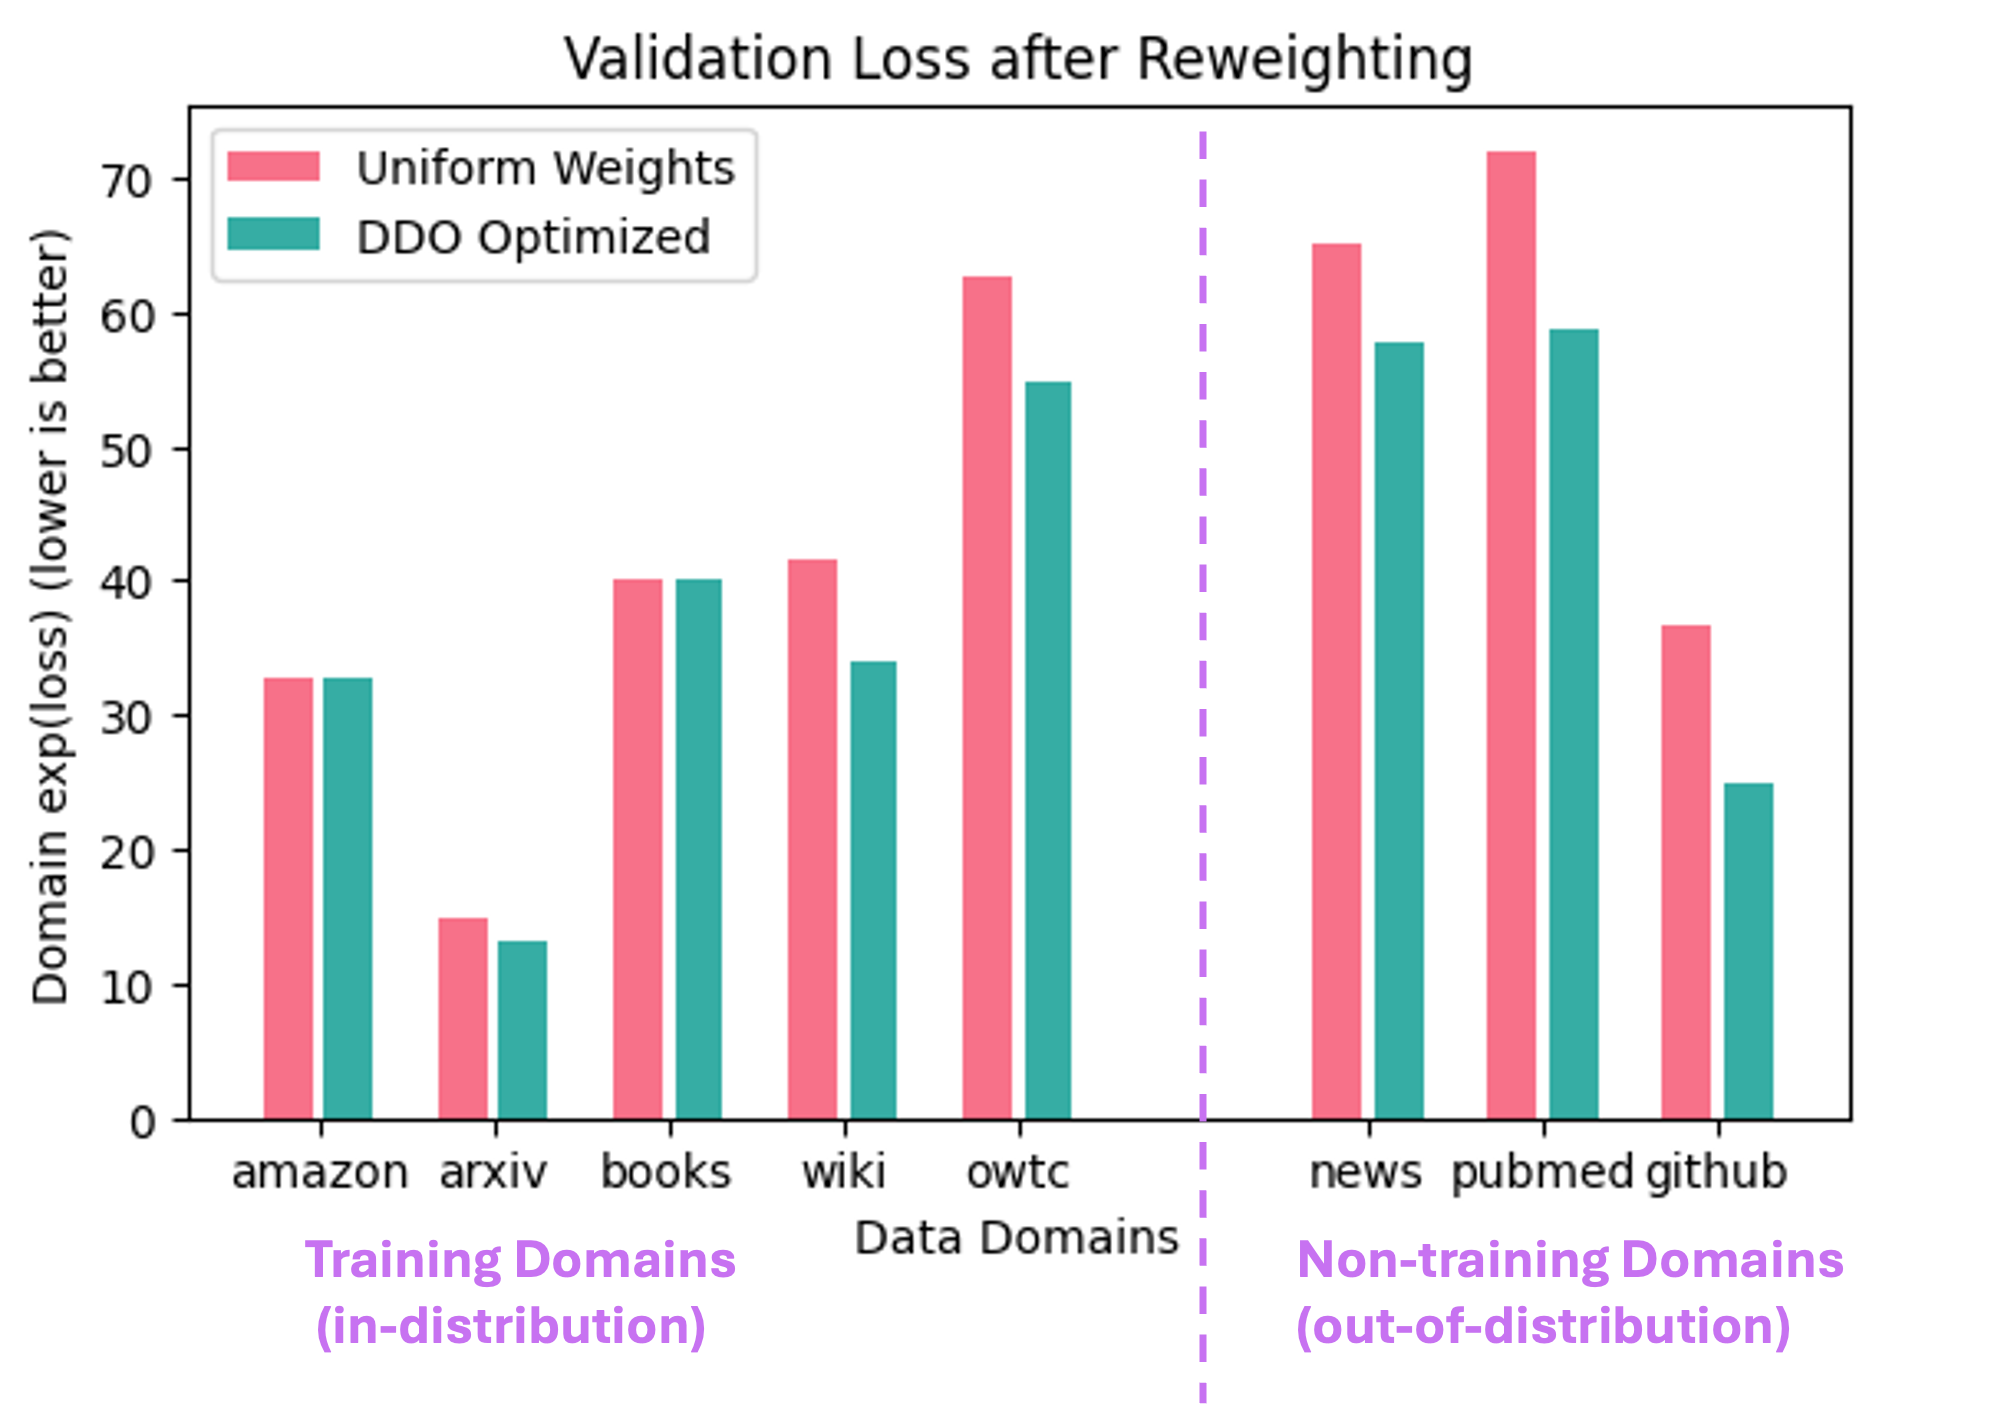
\includegraphics[width=\textwidth]{bertfigs/bert180pr.png}
        \caption{Validation Loss ($\downarrow$ lower is better)}
        \label{fig:figure2a}
    \end{subfigure}
    % \hfill
    % \hspace{1em}
    \begin{subfigure}[b]{0.48\textwidth}
        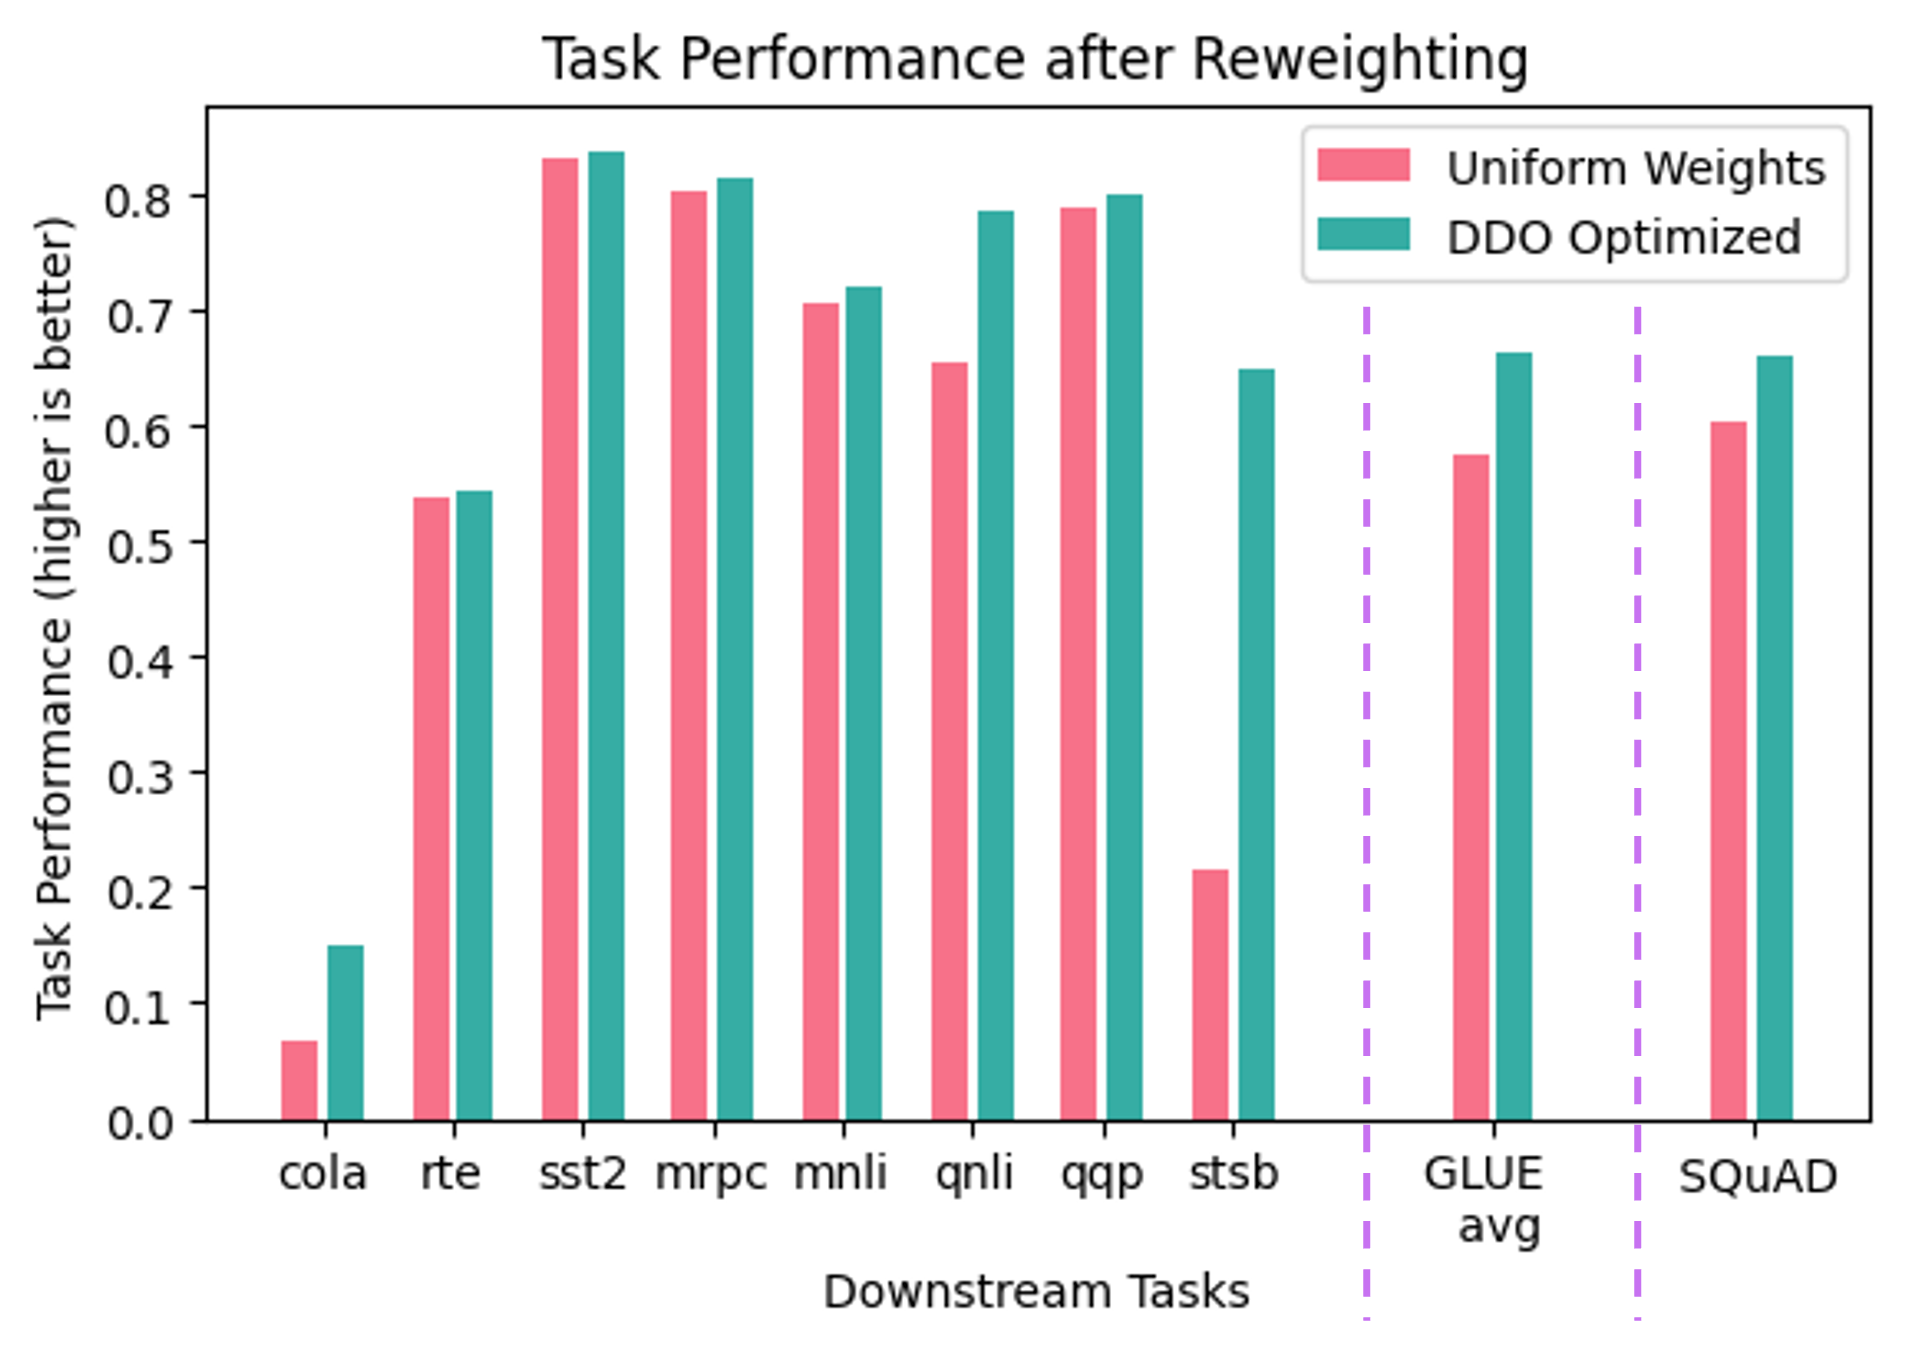
\includegraphics[width=\textwidth]{bertfigs/glue180pr.png}
        \caption{Task Performance ($\uparrow$ higher is better)}
        \label{fig:figure2b}
    \end{subfigure}\vspace{-0.5em}
    \caption{\small{Optimizing domain weights with \textsc{DDO} algorithm for pre-training Encoder-only LMs (\texttt{BERT}). \textsc{DDO} substantially reduces validation loss. After reweighting, all training domains' loss has either decreased or remained unchanged. Out-of-domain loss on non-training domains has also decreased considerably. Enhanced performance ishas been observed on all \texttt{GLUE} tasks (eval metric: \texttt{cola}: Matt. corr., \texttt{stsb}: Pearson corr., rest: acc.) and \texttt{SQuAD} (acc.). }\normalsize}
    \label{fig:figure2}\vspace{-0.5em}
\end{figure}
% For additional results see App.~\ref{sec:appendix_additional_results_bert}.





\textbf{Predicting Optimal Weights at Larger Scales with \textsc{AutoScale}:}
With \textsc{DDO}-optimized weights from models trained up to 0.5B tokens, we fit \textsc{AutoScale} predictor and use it to predict how the optimal domain weights will shift as we continue scaling up training data. Depicted in Fig.~\ref{fig:bert_additional}, similar to the pattern described above, as the training data scale grows, data sources with diverse examples, such as WebText and Amazon Reviews, become increasingly important over standard domains, such as Wikipedia and Arxiv. One hypothesis is such data sources contain samples on diverse topics and language styles, providing rich information compared to domains with clean, standard text.
We train models with MLM for up to 288k steps ($\sim120\%$ of the pertaining data size for original \texttt{BERT-base} \citep{devlin2018bert}). Table \ref{table10} shows that, compared to without reweighting (uniform weights), \textsc{AutoScale}\textit{-predicted weights speed up training by 16.7\% on most data scales with a 10\% speedup on the largest scale, validating its consistent effectiveness}.
\textit{\textcolor{teal}{Takeaway 4: nonetheless, the speedup is less impressive than in the results for Decoder-only LMs, demonstrating the different response to domain reweighting for models with different architecture or language modeling objectives}.} This is also hinted in Fig.~\ref{fig:figure30}(b), where the evaluation loss has a similar response to data from different domains, suggesting limited potential for performance improvements from domain reweighting. 



\vspace{-0.5em}\section{Conclusions}\vspace{-0.5em}
In this work, we demonstrate that the optimal data composition for a fixed compute budget varies depending on the scale of the training data, showcasing that the common practice of empirically determining an optimal composition using small-scale experiments will not yield the optimal data mixtures when scaling up to the final model. Addressing this challenge, we propose \textsc{AutoScale}, an automated tool that finds a compute-optimal data composition for training at any desired target scale. In empirical studies with pre-training 774M Decoder-only LMs and Encoder-only LMs, \textsc{AutoScale} decreases validation perplexity at least 28\% faster than any baseline with up to 38\% speed up compared to without reweighting, achieving the best overall performance across downstream tasks. 
% \subsection{Limitations and Future Work}
% \kang{help here}
% {Bingbing' version, please rewrite it if needed}

\vspace{-0.7em}\paragraph{Limitations $\&$ Future Work} The promising results achieved by \textsc{AutoScale} in optimizing data composition for large-scale language model pretraining open up some intriguing avenues for future exploration.
(1) \textit{Generalizability}: It will be interesting to extend this research to larger-scale settings, other data modalities, and more comprehensive evaluation benchmarks, and re-examine the validity of insights provided by experiments at the scale that we work on.
(2) \textit{Direct optimization of downstream performance}: In practice, the capabilities of LLMs are characterized by their performance on various downstream tasks, and the perplexity loss that we focused on in this study is only a rough, inaccurate proxy for downstream performance. It will be interesting to extend \textsc{AutoScale} to directly optimize downstream performance.
(3) \textit{More fine-grained data curation}: \textsc{AutoScale} works with fixed data domains and only optimizes how the domains are mixed together, confining the optimization space. Intuitively, if one can strategically select the corpus within each domain and even adapt the data selection strategy to different stages of training, further improvements could be achieved.


% \noindent{Fixed Compute Budget.} \textsc{AutoScale} is designed to work within a fixed compute budget, which may not fully capture the complexities of real-world scenarios where compute resources can vary dynamically. Future work could explore adaptive mechanisms that adjust to changing resource availability.

% \noindent{Data Quality and Diversity.} \textsc{AutoScale} does not explicitly account for the intrinsic quality of the data, which can significantly impact model performance. Integrating metrics that assess the intrinsic quality of data into the \textsc{AutoScale} framework could further optimize data composition.

% \noindent{Evaluation on Downstream Tasks.} Although \textsc{AutoScale} shows significant improvements on benchmarks like GLUE and SQuAD, a more comprehensive evaluation across a broader range of downstream tasks and domains would provide a more holistic understanding of its benefits and limitations. 

\paragraph{Broader Impacts}
% \kang{help here} {Bingbing' version, please rewrite it if needed}
Reducing the complexity and resource requirements associated with pretraining LLMs, \textsc{AutoScale} contributes to the democratization of AI. Smaller organizations, academic institutions, and individual researchers can more easily participate in cutting-edge AI research and development, fostering innovation and collaboration across the AI community.  Moreover, learning from massive amounts of data requires large and costly computational resources, which not only consume substantial energy but also generate a significant carbon footprint, contributing to environmental issues. Furthermore, these resources quickly become obsolete due to the rapid pace of technological advancements, leading to e-waste. This research makes contributions to mitigating these issues by improving the efficiency of resource utilization in AI training.

\section*{Acknowledgement}
This work is supported in part by the National Science Foundation under grants IIS-2312794, IIS2313130, OAC-2239622, Amazon-Virginia Tech Initiative in Efficient and Robust Machine Learning, AWS computational credits, and the Commonwealth Cyber Initiative. The authors are grateful for Ankit Battawar and Alix Delgado from AWS, whose dedicated help and support were crucial for securing computing resources and implementing empirical studies.



\newpage

% \section*{Reference}
% \bibliographystyle{unsrt}
% \bibliographystyle{plain} 
\bibliographystyle{plainnat}
\bibliography{iclr2025_conference}

\newpage
\appendix

\appendix{}

\appendixpage{}

\begin{appendices}{}

\startcontents[sections]
\printcontents[sections]{l}{1}{\setcounter{tocdepth}{2}}

\newpage


\section{Extended Related Work}
\label{appendix_related_work}


% Besides, we compare with 2 domain weights from existing research, which are optimized on the same data domains \texttt{RedPajama} dataset with similar Decoder-only LMs. Data Mixing Laws \citep{ye2024data} first performs a grid search on the space of possible data mixtures and records evaluation loss for proxy models trained on these mixtures. Then, the loss is interpolated with exponential functions to find the optimal domain weights for the proxy model. \citep{fan2023doge} also implements DoReMi \citep{xie2024doremi} with auxiliary models trained for 50k steps but with the reference model trained with uniform weights. We evaluate the model trained on these domain weights to present a complete landscape.\kang{too long}


% DoReMi \citep{xie2024doremi} presents a novel approach by optimizing domain weights using a proxy model to minimize the worst-case excess loss across different domains. DoReMi obtains domain weights through the training of two small-scale auxiliary models. Initially, a reference model is well-trained utilizing reference domain weights. \citep{xie2024doremi} shows the performance improvements from optimized domain weights are heavily dependent on the choice of auxiliary models, where using either larger or smaller proxy models is less effective. 

% \citep{fan2023doge}
% [DOGE paper] shows that DoReMi produces very different results when the proxy model is trained on different amounts of data. Additionally, [DOGE paper] argues that the optimized domain weights are independent of parameter size for the proxy model, yet the results show a clear pattern where the optimized domain weights shift consistently with the size of the proxy model.

% A few works emerged during the recent year researching pre-training data curation for LLMs (e.g., \citep{xie2024doremi} [DoReMi], [Skill-it], [Dolma], [Data Mixing Laws], etc.). A majority of these works aim to first optimize data composition for a smaller model and at a smaller data scale (i.e., proxy model/reference model) ([DOGE], [DoReMi], [Data Mixing Laws]). Then, the optimized weights are directly applied to training the target model on magnitudes larger data scales. This implicitly poses a strong assumption that the "optimal data composition" is invariant of model sizes or data scales. Despite its critical role in the development of these approaches, none of these works examines the validity of this assumption. In fact, the design choice of data scale for optimizing the proxy model often has a profound or even uneasy impact on their effectiveness, which has been reported to have inconsistent performance not always surpassing the random baseline. 

% Another common practice is to directly use existing domain weights that were designed for training other models (e.g., LLaMA weights \citep{touvron2023llama}, The Pile weights \citep{gao2020pile}). \citep{mehta2024openelm} recently trained a 1B-parameter model on a combination of [The Pile] dataset, LLaMa (RedPajama) training dataset, and Dolma \citep{soldaini2024dolma} training dataset. These weights are often designed with heuristics [dolma] and/or tuned on downstream tasks [The Pile]. Yet, these weights are optimized for specific applications that may be vastly different from the target scenario. For example, [The Pile] is used to train Pythia Suite/GPT-neo-X model family sizes 14M-12B-parameter and trained on 299.9B tokens. On the other hand, LLaMA-1 and LLaMA-2 are series of 7B-65B-parameter models trained on 1-1.4T tokens and 2T tokens, respectively. These weights need not to be optimal (or even effective) to train, for instance, an 1B-parameter model for 1T tokens, letting alone differences in model architectures or optimizing procedures.


% \paragraph{Data-centric Techniques} 
\textbf{Training Data Curation} Data selection problems have been extensively studied for a variety of applications such as vision~\citep{coleman2019selection, kaushal2019learning, killamsetty2021grad, mindermann2022prioritized}, speech~\citep{park2022unsupervised, rosenberg2023guided}, and language models~\citep{coleman2019selection, mindermann2022prioritized, aharoni2020unsupervised}, and have been attracting growing interest over recent years. For LLMs, a line of research focuses on \textit{data selection for pre-training} (also known as \textit{pre-training data curation})~\citep{brown2020language, gururangan2020don, hoffmann2022training} from scratch or \textit{continued pre-training}. \citep{gururangan2020don} shows that continuing pre-training the model on the domain-specific dataset improves its performance on tasks of this domain; \citep{xie2023data} uses importance resampling on simple bi-gram features with $10$k bins to select millions of samples for domain/task adaptive pre-training.  Problem-specific heuristic methods employ simple criteria to distinguish data quality for a given language model on particular datasets (e.g., via perceived relevance between how the dataset is created and training objectives of the LLM~\citep{chowdhery2022palm}). The effectiveness of these methods for data selection is often limited to specific use cases and easily fails when migrated to different problems \citep{xie2023data}. More recently, \citep{kang2024get} selects samples for fine-tuning pre-trained LLMs via gradients of Optimal Transport distance.
\citep{wettig2024qurating} curates pre-training data using GPT-4 to rate and select samples based on a number of quality criteria; further, \citep{maini2024rephrasing} uses pre-trained LLMs to re-write the entire training corpus to improves its quality for pre-training other LLMs. \citep{albalak2024survey} provides a recent survey for this fast-evolving field. Pre-training data curation is also studied for multimodal foundation models (MMFM)–e.g.,  \citep{mckinzie2024mm1} for vision-language models (VLMs),  and \citep{schuhmann2021laion,goyal2024science} for
CLIP (Contrastive Language-Image Pretraining). 
Aside from pre-training LLMs, domain reweighting problems have been studied in research on collecting data for vision, audio, and text applications \citep{mahmood2022much, mahmood2022optimizing,kang2023performance, just2023asr}.


% \textbf{Data Selection} problems have been extensively studied for a variety of applications such as vision~\citep{coleman2019selection, kaushal2019learning, killamsetty2021grad, mindermann2022prioritized}, speech~\citep{park2022unsupervised, rosenberg2023guided}, and language models~\citep{coleman2019selection, mindermann2022prioritized, aharoni2020unsupervised}, and  have been attracting growing interest over recent years. For LLMs, a line of research focuses on \textbf{data selection for pre-training} (also known as \textbf{pre-training data curation})~\citep{brown2020language, gururangan2020don, hoffmann2022training} from scratch or \textbf{continued pre-training}. For these settings, the scale of data selection budget ranges from millions to billions of samples.  For example, \citep{gururangan2020don} shows that continuing pre-training the model on the domain-specific dataset improves its performance on tasks of this domain; \citep{xie2023data} uses importance resampling on simple bi-gram features with $10$K bins to select millions of samples for domain/task adaptive pre-training.  Problem-specific heuristic methods~\citep{chowdhery2022palm} employ simple criteria to distinguish data quality for a given language model on particular datasets. The effectiveness of these methods for data selection is often limited to specific use cases and easily fails when migrated to different problems \citep{xie2023data}. More recently, \citep{kang2024get} selects samples for fine-tuning pre-trained LLMs via gradients of Optimal Transport distance.
% \citep{wettig2024qurating} curates pre-training data using GPT-4 to rate and select samples based on a number of quality criteria; further, \citep{maini2024rephrasing} uses pre-trained LLMs to re-write the entire training corpus to improves its quality for pre-training other LLMs. Pre-training data curation is also studied for multimodal foundation models (MMFM)–e.g.,  \citep{mckinzie2024mm1} for vision-language models (VLMs),  and \citep{schuhmann2021laion,goyal2024science} for
%CLIP (Contrastive Language-Image Pretraining). Aside from pre-training LLMs, \textbf{Domain Reweighting} problems have been studied in research on collecting data for vision, audio, and text applications \citep{mahmood2022much, mahmood2022optimizing,kang2023performance, just2023asr}.

Besides, \textbf{Coresets} \citep{borsos2020coresets, mirzasoleiman2020coresets} aim to find a representative subset of samples to speed up the training process, which may be formulated as an optimization problem. This process is considerably computationally intensive and hard to be applied on a practical scale for language applications. \textbf{Data Valuation} methods aim to measure the contribution of each sample to the model performance, which naturally provides a viable tool for data selection. Notable examples includes model-based approaches Shapley \citep{jia2019efficient, ghorbani2019data}, LOO \citep{ghorbani2019data, koh2017understanding}, and model-agnostic methods \citep{just2023lava, kwon2023data}. Achieving fruitful results in their respective applications and providing valuable insights, though, these methods are commonly known for their scalability issues. Model-based approaches require repetitive model training and often struggle to apply to a few thousand samples. A recent example, \citep{schoch2023data} uses a sampling approach to speed up a Shapley-style method for selecting data for fine-tuning LLMs and scales up to selecting from $7.28$k subsets. It is hardly imaginable to apply it to the scale of practical language datasets. \citep{just2023lava} utilizes the gradients of an Optimal Transport problem to provide an efficient measure of data values, yet the selection based on gradients does not necessarily align with the target distribution, resulting in mediocre performance in general cases. 



\section{Operational Pipeline for Algorithms}
\label{app:operation}

\begin{figure}[h!]
\begin{center}
  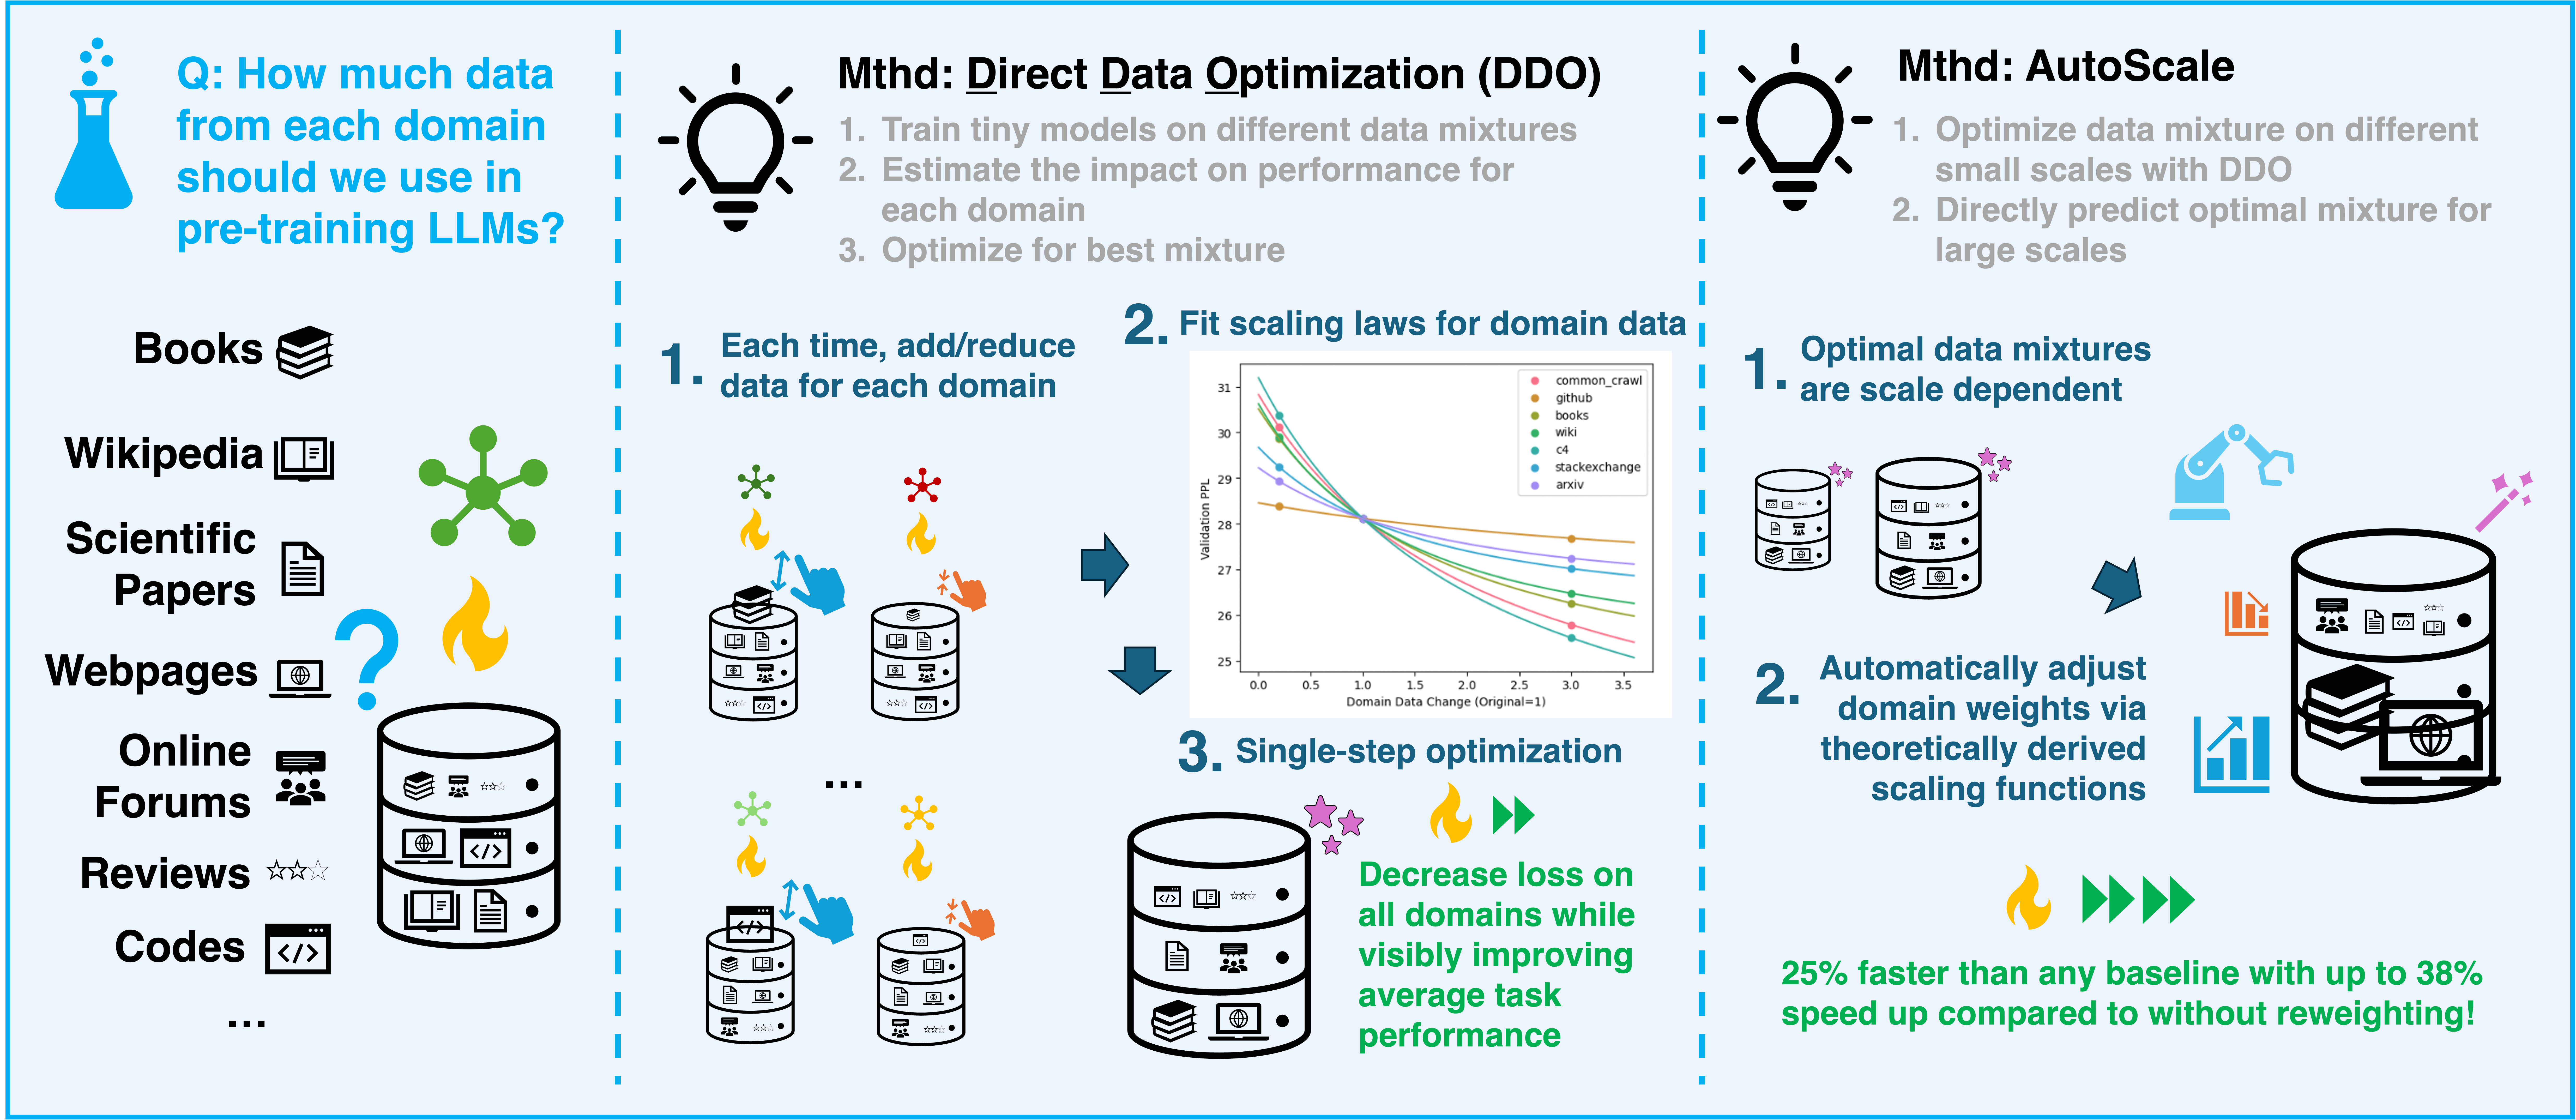
\includegraphics[width=1.0\textwidth]{figs/main_fig_crop.png}
  % \vspace{-1em}
  \caption{LLMs are pre-trained using data from different sources or domains, yet determining the optimal data composition is challenging. We propose \textsc{AutoScale}, an automated tool that finds a compute-optimal data composition for training at any desired target scale. \textsc{AutoScale} first determines the optimal composition at a small scale using a novel bi-level optimization framework, \underline{D}irect \underline{D}ata \underline{O}ptimization (\textsc{DDO}), and then fits a predictor to estimate the optimal composition at larger scales. The predictor's design is inspired by our theoretical analysis of scaling laws related to data composition, which could be of independent interest. In empirical studies, \textsc{AutoScale} decreases validation perplexity at least 25\% faster than any baseline with up to 38\% speed up compared to without reweighting, achieving the best overall performance across downstream tasks. 
  }\label{fig:example}% \vspace{-2em}
  \end{center}
\end{figure}% \vspace{-1em}

\textbf{Operational Pipeline (\textsc{DDO})}
\begin{enumerate}
\item Train a base proxy model with uniform weights (or reference weights, if available);
\item At each time, add/reduce data quantity for one domain and re-train the proxy model;
\item Fit power law scaling functions and solve the optimization problem;
\item Iterate the process if necessary.
\end{enumerate}



\textbf{Operational Pipeline (\textsc{AutoScale})}
\begin{enumerate}

\item For two smaller training data scales $N^{(1)}$ and $N^{(2)}$ where re-training the model is affordable, find their corresponding optimal training data compositions $\mathbf{N^{(1)*}}$ and $\mathbf{N^{(2)*}}$ using \textsc{DDO} Algorithm described above;

\item Predict the next optimal training data composition as $\mathbf{N^{(3)*}} = \mathbf{N^{(2)*}}(\mathbf{N^{(1)*}})^{-1}\mathbf{N^{(2)*}}$, yielding optimal domain weights $w_i^{(3)*}=N_i^{(3)*}/N^{(3)}$ at new training data scale $N^{(3)}=\sum_i N_i^{(3)*}$;
\item Repeat this process until the target training data scale is reached.
\end{enumerate}



\section{Proofs for Sec.~\ref{sec:scaling}}
\label{sec:appendix_proofs}


\subsection{Theorem 1: Scaling Law for Optimal Data Compositions}\label{app:lemma1}
\renewcommand{\thetheorem}{1}
\begin{theorem} [Scaling Law for Optimal Data Compositions \textbf{(restated)}]
    Consider the following optimization problem
    \begin{align*}
        \min_{\mathbf{N}} \left\{ \sum_{i=1}^m \beta_i N_i^{-\gamma_i} \Bigg| \sum_{i=1}^m N_i = N \right\}
    \end{align*}
    For any two compute budgets $N^{(1)} \neq N^{(2)}$, let $\mathbf{N}^{(1)*}$ and $\mathbf{N}^{(2)*}$ be their respective minimizers. 
    Then, there always exists some third data composition $ \mathbf{N}^{(3)*} = \mathbf{N}^{(2)*}(\mathbf{N}^{(1)*}) ^{-1} \mathbf{N}^{(2)*}$ such that $\mathbf{N}^{(3)*}$ is the minimizer for data budget $N^{(3)}=\sum_{i=1}^m N^{(3)}_i$, given as 
         $
        \mathbf{N}^{(3)*} = \arg\min_{\mathbf{N}} \left\{ \sum_{i=1}^m \beta_i N_i^{-\gamma_i} \Bigg| \sum_{i=1}^m N_i = N^{(3)} \right\}.
    $
    % Then, for any third compute budget $N^{(3)}$ such that $N^{(1)} \neq N^{(3)} \neq N^{(2)}$, the corresponding minimizer $\mathbf{N}^{(3)*}$ must satisfy $ \mathbf{N}^{(3)*} = \mathbf{N}^{(2)*}(\mathbf{N}^{(1)*}) ^{-1} \mathbf{N}^{(2)*}$.
\end{theorem}


\begin{proof} For the evaluation loss given as 
\begin{equation*}
\mathcal{L}
=\sum_{i=1}^m \beta_i\cdot N_i^{-\gamma_i},
\end{equation*}
at an optimal data composition, KKT condition \citep{bertsekas1997nonlinear} gives that
we have the partial derivative of the loss function w.r.t. the amount of data from each domain equal to each other. This gives, for any two domains $a$ and $b$ (w.l.o.g, we simplify the derivation to the case of two domains) with optimal data quantity $N_a^*$ and $N_b^*$, respectively, we have
\begin{equation*}
\begin{aligned}
&\frac{\partial\mathcal{L}}{\partial N_a}=-\beta_a\cdot\gamma_a\cdot N_a^{-\gamma_a-1}\\
&\frac{\partial\mathcal{L}}{\partial N_b}=-\beta_b\cdot\gamma_b\cdot N_b^{-\gamma_b-1} \\
&\left.\frac{\partial\mathcal{L}}{\partial N_a}\right|_{N_a=N_a^*}= \left.\frac{\partial\mathcal{L}}{\partial N_b}\right|_{N_b=N_b^*}
\end{aligned}
\end{equation*}

With straightforward derivations, this gives
\begin{equation}\label{eq:nanb}
\begin{aligned}
-\beta_a\cdot\gamma_a\cdot (N_a^*)^{-\gamma_a-1} &=-\beta_b\cdot\gamma_b\cdot (N_b^*)^{-\gamma_b-1} \\
\frac{\beta_a\cdot\gamma_a}{\beta_b\cdot\gamma_b}&=\frac{(N_a^*)^{\gamma_a+1}}{(N_b^*)^{\gamma_b+1}} \\
(N_a^*)^{\gamma_a+1}&=\frac{\beta_a\gamma_a}{\beta_b\gamma_b}(N_b^*)^{\gamma_b+1}\\
N_a^*&=\left[\frac{\beta_a\gamma_a}{\beta_b\gamma_b} (N_b^*)^{\gamma_b+1}\right]^{\frac{1}{\gamma_a+1}}
\end{aligned}
\end{equation}

Let $N_a^{(2)*},N_b^{(2)*}$ be the optimal data quantity for domains $a$ and $b$ at a \textit{different data scale} $N^{(2)}=N_a^{(2)*}+N_b^{(2)*}\neq N$. Assuming we have the optimal data quantity for domain $b$ becoming $m$ times than $N_b^*$, namely, 
\begin{equation*}
\begin{aligned}
N_b^{(2)*}&:=m\cdot N_b^*
\end{aligned}
\end{equation*}
Then, from Eq. \ref{eq:nanb}, the optimal data quantity for domain $a$ can be given as
\begin{equation}\label{eq:naprime}
\begin{aligned}
N_a^{(2)*}&=\left[\frac{\beta_a\gamma_a}{\beta_b\gamma_b}(N_b^{(2)*})^{\gamma_b+1}\right]^{\frac{1}{\gamma_a+1}} \\
&=\left[\frac{\beta_a\gamma_a}{\beta_b\gamma_b}(m\cdot N_b^*)^{\gamma_b+1}\right]^{\frac{1}{\gamma_a+1}} \\
&=m^{\frac{\gamma_b+1}{\gamma_a+1}}\cdot\left[\frac{\beta_a\gamma_a}{\beta_b\gamma_b}(N_b^*)^{\gamma_b+1}\right]^{\frac{1}{\gamma_a+1}} \\
&= m^{\frac{\gamma_b+1}{\gamma_a+1}}\cdot N_a^* % \\
% \log N_a' &= \frac{\gamma_b+1}{\gamma_a+1}\log m + \log N_a \\
% \log N_b' &= \log m + \log N_b
\end{aligned}
\end{equation}


It can be immediately seen that the optimal domain data $N_a^*$ and $N_b^*$ scale at different rates–new optimal data quantity for domain $a$ \textit{does not} become $m$ times than before. 
This implies that the optimal data composition is scale-dependent and is different for different training data scales. 
This implies that the optimal data composition is scale-dependent and is different for different training data scales, establishing the main argument of this paper.

Since the ratio from Eq. \ref{eq:naprime}, $(\gamma_b+1)/(\gamma_a+1)$, is constant and invariant to the change in the training data scale, it can be utilized to provide a direct approach for predicting the scaling of optimal data compositions–given as
\begin{equation*}
    N_a^{(2)*} = (\frac{N_b^{(2)*}}{N_b^*})^{{\frac{\gamma_b+1}{\gamma_a+1}}}N_a^*
\end{equation*}
Equivalently, taking the logarithm for both sides of the equation, we have
\begin{equation*}
    \log N_a^{(2)*} = \log(\frac{N_b^{(2)*}}{N_b^*})^{{\frac{\gamma_b+1}{\gamma_a+1}}} + \log  N_a^*
\end{equation*}

Further, we show that one \textit{does not} need to estimate any of the coefficients ($\gamma_a$, $\gamma_b$) from the loss function to predict the optimal data quantity for each domain. 
Assume one have obtained the optimal data quantity for domains $a$ and $b$, $N_a^{(1)*},N_b^{(1)*}$, at a \textit{data scale} $N^{(1)}=N_a^{(1)*}+N_b^{(1)*}$ and the optimal data quantity $N_a^{(2)*},N_b^{(2)*}$  at a \textit{data scale} $N^{(2)}=N_a^{(2)*}+N_b^{(2)*}$ where $ N^{(1)} \neq N^{(2)}$. This gives
\begin{equation*}
    \log N_a^{(2)*} = \frac{\gamma_b+1}{\gamma_a+1} \cdot (\log N_b^{(2)*}-\log N_b^{(1)*})  + \log  N_a^{(1)*}
\end{equation*}
Then, for a different data scale where the optimal data quantity for domain $b$ is $N_b^{(3)*}$, the optimal data quantity for domain $a$ can be given as
\begin{equation*}
\begin{aligned}
    \log N_a^{(3)*} =& \frac{\gamma_b+1}{\gamma_a+1} \cdot (\log N_b^{(3)*}-\log N_b^{(2)*})  + \log  N_a^{(2)*}\\
    =&\frac{\log  N_a^{(2)*}-\log  N_a^{(1)*}}{\log N_b^{(2)*}-\log N_b^{(1)*}}\cdot (\log N_b^{(3)*}-\log N_b^{(2)*})  + \log  N_a^{(2)*}
\end{aligned}
\end{equation*}

W.l.o.g., consider $\frac{N_b^{(3)*}}{N_b^{(2)*}}=\frac{N_b^{(2)*}}{N_b^{(1)*}}$
where $\log N_b^{(2)*}-\log N_b^{(1)*}=\log N_b^{(3)*}-\log N_b^{(2)*}$, the equation above can be simplified to
\begin{equation*}
    \log N_a^{(3)*} = 2\log N_a^{(2)*} - \log N_a^{(1)*}
\end{equation*}
and equivalently,
\begin{equation*}
    N_a^{(3)*} = \frac{(N_a^{(2)*})^2}{N_a^{(1)*}}
\end{equation*}

Defining compact representations $\mathbf{N^{(i)*}}=diag\{N_a^{(i)*},N_b^{(i)*}\}$, the above results can be written as
\begin{equation*}
    \mathbf{N^{(3)*}}=\mathbf{N^{(2)*}}(\mathbf{N^{(1)*}})^{-1}\mathbf{N^{(2)*}}
\end{equation*}
which concludes the proof.


The process can be iterated (e.g., replacing $\mathbf{N^{(1)*}}$ or $\mathbf{N^{(2)*}}$ with $\mathbf{N^{(3)*}}$) to obtain optimal domain data quantity for different data scales.
 The example below provides a straightforward look on how this result can be operationalized.
% It can be seen that the ratio $(\gamma_b+1)/(\gamma_a+1)$ is constant and invariant to the change in data scales $N=N_a+N_b$. This provides a direct approach for predicting the scaling of optimal data compositions.
\end{proof}

\begin{remark} [An example]
    This example helps visualize the operation pipeline. 
    
    If at training data scale $N^{(1)}=N_a^{(1)}+N_b^{(1)}=200$, we have optimal domain data composition as $N_a^{(1)*}=100, N_b^{(1)*}=100$ ($50\%-50\%$); and at scale $N^{(2)}=N_a^{(2)}+N_b^{(2)}=500$, we have optimal domain data composition as $N_a^{(2)*}=300, N_b^{(2)*}=200$ ($60\%-40\%$). Then, from the theorem, when the optimal domain data composition has $N_a^{(3)*}=(N_a^{(2)*})^2/N_a^{(1)*}=900$, we can predict $N_b^{(3)*}=(N_b^{(2)*})^2/N_b^{(1)*}=400$, which gives the optimal ratio at $N^{(3)}=N_a^{(3)}+N_b^{(3)}=1300$ as $69\%-31\%$. 
    
    Similarly, 
    
\small 
% For $N_a^{(1)*}=100$, we have $N_b^{(1)*}=100$, which gives the optimal ratio at $N^{(1)}=200$ as $50\%-50\%$\\
% For $N_a^{(2)*}=300$, we have $N_b^{(2)*}=200$, which gives the optimal ratio at $N^{(2)}=500$ as $60\%-40\%$\\
% For $N_a^{(3)*}=900$, we have $N_b^{(3)*}=400$, which gives the optimal ratio at $N^{(3)}=1300$ as $69\%-31\%$\\
For $N_a^{(4)*}=2700$, we have $N_b^{(4)*}=800$, which gives the optimal ratio at $N^{(4)}=3500$ as $77\%-23\%$\\
For $N_a^{(5)*}=8100$, we have $N_b^{(5)*}=1600$, which gives the optimal ratio at $N^{(5)}=9700$ as $84\%-16\%$\\
For $N_a^{(6)*}=24300$, we have $N_b^{(6)*}=3200$, which gives the optimal ratio at $N^{(6)}=27500$ as $88\%-12\%$\\
For $N_a^{(7)*}=72900$, we have $N_b^{(7)*}=6400$, which gives the optimal ratio at $N^{(7)}=79300$ as $92\%-8\%$\\
For $N_a^{(8)*}=218700$, we have $N_b^{(8)*}=12800$, which gives the optimal ratio at $N^{(8)}=231500$ as $94\%-6\%$\\
For $N_a^{(9)*}=656100$, we have $N_b^{(9)*}=25600$, which gives the optimal ratio at $N^{(9)}=681700$ as $96\%-4\%$\normalsize

We visualize it in Fig.~\ref{fig:example}.
\begin{figure}[h!]
\begin{center}
  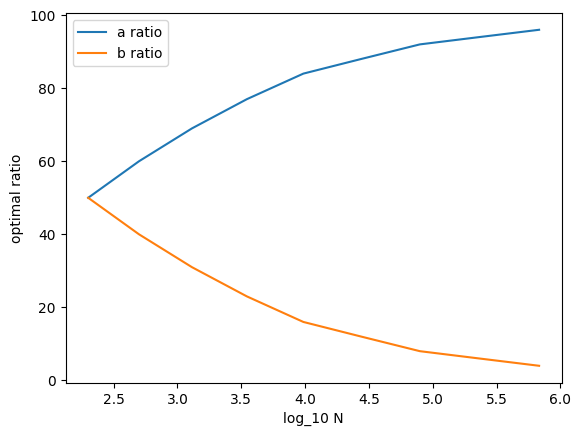
\includegraphics[width=0.7\textwidth]{figs/abratio.png}
  \vspace{-1em}
  \caption{Illustration: optimal data composition scales in exponential-style functions with training data quantity.
  }\label{fig:example}
  \vspace{-1em}
  \end{center}
\end{figure}% \vspace{-1em}
\end{remark}




\subsection{Scaling Latent Skills}\label{app:theorem1}
We extend this theory to a general case where the evaluation loss is the perplexity averaged over training domains.
Consider the evaluation is composed of a number of \textit{independent} sub-tasks ("latent skills" \citep{tiong2024toward}) which are hidden variables, where each of them observes a power law scaling law relationship with the amount of data contributing to this task ("equivalent data size"), $
\mathcal{L} =\ell_0+\beta_a\cdot K_a^{-\gamma_a}+\beta_b\cdot K_b^{-\gamma_b}+\beta_c\cdot K_c^{-\gamma_c} + \cdots
$
where scalar $K_j\geq 0$ denote equivalent data size for \textit{skill$_j$}, and constants $(\beta_j, \gamma_j)\geq 0$ are coefficients associated with \textit{skill$_j$}, respectively. Mathematically, these latent skills can be seen as an orthogonal basis that spans the space of evaluation loss.

Consider training data from each domain $D_i$ contributes to these skills to varying degrees, where Equivalent data size for \textit{skill$_j$}, $K_j$, is given as
$
K_j = c_{j,1}\cdot N_1 + c_{j,2}\cdot N_2 + \cdots
$
where $N_i=w_i\cdot N$ denotes the amount of training data from domain $D_i$ and constant $c_{j,i}$ is the coefficient measuring the degree of contribution between domain $D_i$ and \textit{skill$_j$}.
Defining diagonal matrices for training data composition $\mathbf{N}=diag\{N_1,N_2, \cdots\}$ and skill data composition $\mathbf{K}=diag\{K_a,K_b,\cdots\}$, we have 
$
\mathbf{K} = \mathbf{A}\mathbf{N}
$,
where $\mathbf{A}_{ji}=c_{j,i}$ is the matrix for coefficients. 
For simplicity, we consider training data from each domain will be \textit{distributed} to the skills such that $\forall i, \sum_j N_i = 1 $. This gives the amount of total training data from all domains is identical to the amount of total equivalent data for all skills, $\sum_j K_j = \sum_i N_i$.
For a training data scale $N=\sum_i N_i=\sum_j K_j$, define optimal skill data composition $\mathbf{K^*}=diag\{K_a^*, K_b^*, \cdots\}$ as the minimizer of $\mathcal{L}$, given as
$
    \mathbf{K^*} = {\arg\min}_{\sum_j K_j=N} \ell_0+\beta_a\cdot K_a^{-\gamma_a}+\beta_b\cdot K_b^{-\gamma_b}+ \cdots
$. 
Theoretically, there can be an infinite number of latent skills. For analysis, we consider a finite number of $k$ independent skills \textit{most important} for the evaluation. This can considered as performing Principal Components Analysis (PCA) with orthogonal transformation and selecting the first $k$ independent components. We consider the standard scenario with an equal number of relevant skills and data domains where $k=m$ and $\mathbf{A}$ is a square matrix with full rank. This describes the case where this optimization problem is well-defined. We discuss in App.~\ref{app:theorem1} what will happen in other scenarios. 
In this case, $\mathbf{A}$ is invertible and the corresponding optimal training data composition for $\mathbf{K^*}$ can be given as
$
\mathbf{N^*} =  \mathbf{A}^{-1}\mathbf{K^*}
$.

We provide the following theorem, which states that for the scenario described above, optimal training data composition scales in exponential-style functions with training data quantity and can be directly predictable from that of smaller scales \textit{without needing to identify the latent skills}.

% \renewcommand{\thetheorem}{2}
% \begin{theorem} [Scaling Latent Skills]
% Consider the evaluation is composed of a number of \textit{independent} sub-tasks ("latent skills") where each of them observes a power law scaling law relationship with the amount of data contributing to this task ("equivalent data size")as described above. 
% If we have optimal data compositions $\mathbf{N^*}=diag\{N_a^*, N_b^*, \cdots\}$ 
% where its corresponding skill data composition $\mathbf{K^*}=diag\{K_a^*, K_b^*, \cdots\}=\mathbf{A}\mathbf{N^*}$ minimizes $\mathcal{L}$ s.t. $\sum_j K_j=\sum_i N^*=N$, and $\mathbf{N^{'*}}=diag\{N_a^{'*}, N_b^{'*}, \cdots\}$ 
% where its corresponding skill data composition $\mathbf{K^{'*}}=diag\{K_a^{'*}, K_b^{'*}, \cdots\}=\mathbf{A}\mathbf{N^{'*}}$ minimizes $\mathcal{L}$ s.t. $\sum_j K_j'=\sum_i N^{'*}=N'$ where $N'\neq N$, then, other optimal data compositions $\mathbf{N^{''*}}=diag\{N_a^{''*}, N_b^{''*}, \cdots\}$ 
% where its corresponding skill data composition $\mathbf{K^{''*}}=diag\{K_a^{''*}, K_b^{''*}, \cdots\}=\mathbf{A}\mathbf{N^{''*}}$ minimizes $\mathcal{L}$ s.t. $\sum_j K_j''=\sum_i N^{''*}=N''$ where $N''\neq N'\neq N$ can be given as
% $
% \mathbf{N''} = (\mathbf{N'})^{-1}\mathbf{N}\mathbf{N'}
% $.
% \end{theorem}
%     See App.~\ref{app:theorem1} for the formal statement and proof.



% \subsection{Theorem 1: Scaling Latent Skills}\label{app:theorem1}

\renewcommand{\thetheorem}{2}
\begin{theorem} [Scaling Latent Skills]
Consider the evaluation is composed of a number of \textit{independent} sub-tasks ("latent skills") where each of them observes a power law scaling law relationship with the amount of data contributing to this task ("equivalent data size"). Namely, 
$
\mathcal{L} =\ell_0+\beta_a\cdot K_a^{-\gamma_a}+\beta_b\cdot K_b^{-\gamma_b}+\beta_c\cdot K_c^{-\gamma_c} + \cdots
$
where scalar $K_j\geq 0$ denote equivalent data size for \textit{skill$_j$}, and constants $(\beta_j, \gamma_j)\geq 0$ are coefficients associated with \textit{skill$_j$}, respectively.
Define diagonal matrices for training data composition $\mathbf{N}=diag\{N_1,N_2, \cdots\}$ and skill data composition $\mathbf{K}=diag\{K_a,K_b, \cdots\}$. Consider training data from each domain $D_i$ contributes to these skills to varying degrees, given as $\mathbf{K} = \mathbf{A}\mathbf{N}$ where $\mathbf{A}_{ji}=c_{j,i}$ is the matrix for coefficients. 
Assume the amount of total training data from all domains is identical to the amount of total equivalent data for all skills, $\sum_j K_j = \sum_i N_i$. Assume there is a finite number of latent skills and data domains and $\mathbf{A}$ is a square matrix with full rank. 
For a training data scale $N=\sum_i N_i=\sum_j K_j$
, define optimal skill data composition $\mathbf{K^*}=diag\{K_a^*, K_b^*, \cdots\}$ as the minimizer of $\mathcal{L}$ s.t. $\sum_j K_j=N$ with corresponding optimal training data composition 
If we have optimal data compositions $\mathbf{N^{(1)*}}=diag\{N_a^{(1)*}, N_b^{(1)*}, \cdots\}$ 
where its corresponding skill data composition $\mathbf{K^{(1)*}}=diag\{K_a^{(1)*}, K_b^{(1)*}, \cdots\}=\mathbf{A}\mathbf{N^{(1)*}}$ minimizes $\mathcal{L}$ s.t. $\sum_j K_j=\sum_i N^{(1)*}=N^{(1)}$, and $\mathbf{N^{(2)*}}=diag\{N_a^{(2)*}, N_b^{(2)*},...\}$ 
where its corresponding skill data composition $\mathbf{K^{(2)*}}=diag\{K_a^{(2)*}, K_b^{(2)*},...\}=\mathbf{A}\mathbf{N^{(2)*}}$ minimizes $\mathcal{L}$ s.t. $\sum_j K_j^{(2)*}=\sum_i N^{(2)*}=N^{(2)}$ where $N^{(2)}\neq N^{(1)}$, then, other optimal data compositions $\mathbf{N^{(3)*}}=diag\{N_a^{(3)*}, N_b^{(3)*},...\}$ 
where its corresponding skill data composition $\mathbf{K^{(3)*}}=diag\{K_a^{(3)*}, K_b^{(3)*}, \cdots\}=\mathbf{A}\mathbf{N^{(3)*}}$ minimizes $\mathcal{L}$ s.t. $\sum_j K_j^{(3)*}=\sum_i N^{(3)*}=N^{(3)}$ where $N^{(3)}\neq N^{(2)}\neq N^{(1)}$ can be given as
$
\mathbf{N^{(3)*}} = \mathbf{N^{(2)*}}(\mathbf{N^{(1)*}})^{-1}\mathbf{N^{(2)*}}
$.
\end{theorem}
\begin{proof}
By definition, we have
    \begin{equation*}
\begin{aligned}
\mathbf{A}\mathbf{N^{(1)*}} = \mathbf{K^{(1)*}},\quad
\mathbf{A}\mathbf{N^{(2)*}} = \mathbf{K^{(2)*}},\quad
\mathbf{A}\mathbf{N^{(3)*}} = \mathbf{K^{(3)*}}
\end{aligned}
\end{equation*}
From results of Theorem \ref{thm:thm1n}, we have
\begin{equation*}
    \mathbf{K^{(3)*}}=\mathbf{K^{(2)*}}(\mathbf{K}^{(1)*})^{-1}\mathbf{K^{(2)*}}
\end{equation*}
which gives
\begin{equation*}
    \mathbf{A}\mathbf{N^{(3)*}}=(\mathbf{A}\mathbf{N^{(2)*}})(\mathbf{A}\mathbf{N^{(1)*}})^{-1}\mathbf{A}\mathbf{N^{(2)*}}
\end{equation*}

Since $\mathbf{A}$ is invertible and $\mathbf{N}$ and $\mathbf{K}$ are diagonal matrices, naturally, 
\begin{equation*}
\begin{aligned}
(\mathbf{A}\mathbf{N^{(1)*}})^{-1} = (\mathbf{N^{(1)*}})^{-1}\mathbf{A}^{-1}
\end{aligned}
\end{equation*}
and we have
\begin{equation*}
    \mathbf{A}\mathbf{N^{(3)*}}=\mathbf{A}\mathbf{N^{(2)*}}[(\mathbf{N^{(1)*}})^{-1}\mathbf{A}^{-1}]\mathbf{A}\mathbf{N^{(2)*}}=\mathbf{A}\mathbf{N^{(2)*}}(\mathbf{N^{(1)*}})^{-1}\mathbf{N^{(2)*}}
\end{equation*}

This directly gives
\begin{equation*}
    \mathbf{N^{(3)*}}=\mathbf{A}^{-1}\mathbf{A}\mathbf{N^{(2)*}}(\mathbf{N}^{(1)*})^{-1}\mathbf{N^{(2)*}}=\mathbf{N^{(2)*}}(\mathbf{N}^{(1)*})^{-1}\mathbf{N^{(2)*}}
\end{equation*}
which completes the proof.

% Note that $\mathbf{N'}$ is a diagonal matrix, thus $\mathbf{A}\mathbf{N'}=\mathbf{N'}\mathbf{A}$.

% Then, combining the equations above, it gives
% \begin{equation*}
% \begin{aligned}
% \mathbf{N'} &= \mathbf{A}^{-1}\mathbf{K'}=\mathbf{A}^{-1}\mathbf{X}\mathbf{K}=(\mathbf{A}^{-1}\mathbf{K})\mathbf{X}=\mathbf{N}^{-1}\mathbf{X}
% \end{aligned}
% \end{equation*}
% \begin{equation*}
% \begin{aligned}
% \mathbf{N''} &= \mathbf{A}^{-1}\mathbf{X}\mathbf{K'}=(\mathbf{A}^{-1}\mathbf{K'})\mathbf{X}=(\mathbf{N}')^{-1}\mathbf{X}
% \end{aligned}
% \end{equation*}

% Straightforwardly, we end up having
% \begin{equation*}
% \begin{aligned}
% \mathbf{N}\mathbf{N'} &= \mathbf{N'}\mathbf{N''}
% \end{aligned}
% \end{equation*}
% which gives
% \begin{equation*}
% \begin{aligned}
% \mathbf{N''} &= (\mathbf{N'})^{-1}\mathbf{N}\mathbf{N'}
% \end{aligned}
% \end{equation*}

The above result does not require identifying the latent skills or observing skill data compositions $\mathbf{K}$. Rather, the theorem gives that as long as the coefficient matrix $\mathbf{A}$ is invertible, the scaling of $\mathbf{N}$ complies to the same scaling law as in Sec.~\ref{sec:33n}.
\end{proof}





% \subsection{B2 full description}
% \subsection{Scaling Latent Skills}
% We built our theory from a stylized example where we assume the evaluation metric is composed of independent tasks with separate scaling laws and each training sample only contributes to a single task. We move on to extend this theory to general cases and demonstrate how it relates to our problem where the evaluation loss is the perplexity averaged over training domains.

% If we consider evaluation loss (perplexity) on each domain as the sub-tasks, the perplexity of different domains is largely not independent. Some commonly used domains overlap to a considerable degree (e.g., CommonCrawl and C4 [add cite]). Yet, each domain often has its unique contribution to the evaluation loss and can not be directly substituted by others. Thus, we instead assume there are latent skills, which are hidden variables, that are sub-tasks of the evaluation that scale independently [add ref on latent skills].
% Consider the evaluation is composed of a number of \textit{independent} sub-tasks ("latent skills") where each of them observes a power law scaling law relationship with the amount of data contributing to this task ("equivalent data size"). Namely, 
% $
% \mathcal{L} =\mathcal{L}_0+\beta_a\cdot K_a^{-\gamma_a}+\beta_b\cdot K_b^{-\gamma_b}+\beta_c\cdot K_c^{-\gamma_c} +...
% $
% where scalar $K_j\geq 0$ denote equivalent data size for \textit{skill$_j$}, and constants $(\beta_j, \gamma_j)\geq 0$ are coefficients associated with \textit{skill$_j$}, respectively. Mathematically, these latent skills can be seen as an orthogonal basis that spans the space of evaluation loss.
% Consider training data from each domain $D_i$ contributes to these skills to varying degrees, where Equivalent data size for \textit{skill$_j$}, $K_j$, is given as
% $
% K_j = c_{j,1}\cdot N_1 + c_{j,2}\cdot N_2 + ...
% $
% where $N_i=w_i\cdot N$ denotes the amount of training data from domain $D_i$ and constant $c_{j,i}$ is the coefficient measuring the degree of contribution between domain $D_i$ and \textit{skill$_j$}.
% Defining diagonal matrices for training data composition $\mathbf{N}=diag\{N_1,N_2...\}$ and skill data composition $\mathbf{K}=diag\{K_a,K_b...\}$, we have 
% $
% \mathbf{K} = \mathbf{A}\mathbf{N}
% $,
% where $\mathbf{A}_{ji}=c_{j,i}$ is the matrix for coefficients. 
% For simplicity, we consider training data from each domain will be \textit{distributed} to the skills such that $\forall i, \sum_j N_i = 1 $. This gives the amount of total training data from all domains is identical to the amount of total equivalent data for all skills, $\sum_j K_j = \sum_i N_i$.
% For a training data scale $N=\sum_i N_i=\sum_j K_j$, define optimal skill data composition $\mathbf{K^*}=diag\{K_a^*, K_b^*,...\}$ as the minimizer of $\mathcal{L}$, given as
% $
%     \mathbf{K^*} = {\arg\min}_{\sum_i K_j=N} \mathcal{L}_0+\beta_a\cdot K_a^{-\gamma_a}+\beta_b\cdot K_b^{-\gamma_b}+...
% $.
% Theoretically, there can be an infinite number of latent skills. For analysis, we consider a finite number of $k$ independent skills \textit{most important} for the evaluation. This can considered as performing Principal Components Analysis (PCA) with orthogonal transformation and selecting the first $k$ independent components. We consider the standard scenario with an equal number of relevant skills and data domains where $k=m$ and $\mathbf{A}$ is a square matrix with full rank. This describes the case where this optimization problem is well-defined. We will later discuss what will happen in other scenarios. 
% In this case, $\mathbf{A}$ is invertible and the corresponding optimal training data composition for $\mathbf{K^*}$ can be given as
% $
% \mathbf{N} =  \mathbf{A}^{-1}\mathbf{K}
% $

% Consider the evaluation is composed of a number of \textit{independent} sub-tasks ("latent skills") where each of them observes a power law scaling law relationship with the amount of data contributing to this task ("equivalent data size"). We provide the following theorem, which states that for the scenario described above, optimal training data composition scales exponentially with training data quantity and can be directly predictable from that of smaller scales \textit{without needing to identify the latent skills}.



    


\begin{remark} [what happens when $\mathbf{A}$ is not invertible.]
In general, if $\mathbf{A}$ is not invertible, scaling for optimal training data composition is not directly predictable. Specifically, if $\mathbf{A}$ does not have full rank, there exists redundant domains/data sources where their contribution to the skills are identical/exact multipliers of each other. Some data sources may not be needed at any scale; if $\mathbf{A}$ has more rows than columns (more domains than skills), this suggests multiple training data compositions can achieve the same skills data composition and the optimal training data compositions are non-unique (infinitely many).
If $\mathbf{A}$ has more columns than rows (more skills than domains), this means there are too many skills to optimize for. No optimal training data composition exists and one has to make trade-offs. If this is relevant to the practical needs, training data may be processed with additional techniques such as clustering and split into more different domains.
\end{remark}

\section{Experimental Details and Additional Results}
\subsection{Experimental Details of Sec.~\ref{sec:exp-gpt}}
\label{sec:appendix_exp_details_gpt}
\paragraph{Model Training}

\texttt{GPT-2 Large} is a variant of the \texttt{GPT-2} architecture, featuring an embedding dimension of 1280, 36 transformer layers, and 20 attention heads. We rely on the Hugging Face Transformers library for implementation \citep{wolf2019huggingface}. Specific training hyperparameters are detailed in Table \ref{tab:gpt2-large hyperparams}.

\begin{table}[h]
\centering{
\begin{tabular}{lr}
\toprule
Architecture & gpt2\\
Optimizer & AdamW \\
 Tokenizer Vocabulary Size&$50257$\\

Batch Size Per Device & $1$\\
 Gradient Accumulation Steps&$10$\\
Maximum Learning Rate & 2e-4\\
LR Schedule & Linear \\
Weight Decay & 1e-2 \\
Warm-up Ratio& $10\%$\\
Epochs & $3$\\
GPU Hardware & 8x NVIDIA A100/8x NVIDIA H100\\
\bottomrule
\end{tabular}
\caption{The list of hyperparameters for \texttt{GPT-2 Large} pretraining.}

\label{tab:gpt2-large hyperparams}}
\end{table} 
% \call{table go to appendix}

% \kang{tokenizer vocabulary size}



\paragraph{Dataset Details}

The \texttt{RedPajama} dataset is available at: \url{https://huggingface.co/datasets/togethercomputer/RedPajama-Data-1T}.
The 7 domains involved are characterized as follows: 
% [list 7 domains, wiki, books, cc, c4 ...]

% \call{ list go to appendix}
\begin{itemize}
\item \textbf{\texttt{Commoncrawl}}: A vast repository of web-crawled data, providing a heterogeneous mix of internet text.
\item \textbf{\texttt{C4}}: The Colossal Clean Crawled Corpus, filtered to remove low-quality content, thus ensuring the reliability and cleanliness of the data.
\item \textbf{\texttt{GitHub}}: This domain includes a compilation of publicly available code repositories, offering a rich source of syntactic and semantic patterns inherent in programming languages.
\item \textbf{\texttt{Books}}: A collection of textual content from published books, providing diverse narrative styles and complex character developments.
\item \textbf{\texttt{ArXiv}}: Comprising scientific papers primarily from the fields of physics, mathematics, computer science, and quantitative biology, this domain offers high-quality, scholarly content.
\item \textbf{\texttt{Wikipedia}}: A well-organized and meticulously curated dataset of encyclopedia articles, delivering a broad spectrum of knowledge across multiple disciplines. We only use English samples with 'en' in meta-data.
\item \textbf{\texttt{StackExchange}}: This domain captures a variety of user-generated content from discussions and question-answer sessions across numerous technical topics.
\end{itemize}
% We apply the following preprocessing procedure to each domain-specific dataset to ensure consistency and quality for the pretraining of \texttt{GPT-2 Large}. \call{appendix}
Given copyright restrictions with the \texttt{Books} domain on Hugging Face, we have opted for an alternative source available at \url{https://yknzhu.wixsite.com/mbweb}.

For each domain, we ensure only samples with more than 1000 characters are retained. For each sample, the first 1000 characters are truncated, with the exception of the \texttt{ArXiv} and \texttt{GitHub} domains where we randomly extract a continuous block of 1000 characters. For the \texttt{Wikipedia} domain, we keep only those samples that are in English. Samples are selected without replacement, based on the computed data volume for each domain. Additionally, for each domain, a held-out dataset comprising 10K samples is reserved to evaluate the perplexity of the pretrained model. 
% \ys{Can go to manuscript if space allows}
% \call{appendix}

\subsection{Experimental Details of Sec.~\ref{sec:exp-bert}}
\label{sec:appendix_exp_details_bert}


% 5 domains, arXiv, Amazon Reviews, Open Web Text Corpus (OWTC), Wikipedia, books, 
% excluded programming language such as GitHub and StackExchange
% Amazon Reviews for sentiment analysis
% bert-base-uncased training from scratch

\paragraph{Model Training} We employ the \texttt{BERT-base-uncased} model from the Hugging Face Transformers library. Originally, \texttt{BERT}'s pretraining scheme involved MLM and next sentence prediction (NSP); however, in our experiments, we exclusively utilize MLM. Detailed training hyperparameters can be found in Table \ref{tab:bert hyperparams}.
\begin{table}[h]
\centering{
\begin{tabular}{lr}
\toprule
Architecture & bert-base-uncased \\
Max Token Length & $300$ \\
Mask Token Percentage & $15$\% \\
Optimizer & AdamW \\

Batch Size Per Device & $12$ \\
Devices & $4$ \\
Maximum Learning Rate & 1e-4 \\
LR Schedule & Linear \\
Weight Decay & 1e-2 \\
Warm-up Steps & $3000$\\
Epochs & $1\sim4$ \\
GPU Hardware & 4x NVIDIA RTX A6000\\
\bottomrule
\end{tabular}

 \caption{The list of hyperparameters for \texttt{BERT} pretraining.}
\label{tab:bert hyperparams}}
\end{table}


\paragraph{Dataset Details}

The 5 domains of training data utilized are listed as follows:

\begin{itemize}
\item \textbf{\texttt{Amazon Reviews}}: A compilation of customer reviews from Amazon, widely utilized in sentiment analysis studies, available at: \url{https://huggingface.co/datasets/amazon_us_reviews}.
\item \textbf{\texttt{Arxiv}}: Comprises 1.7 million articles from arXiv, available at: \url{https://www.tensorflow.org/datasets/catalog/scientific_papers}.
\item \textbf{\texttt{Books}}: A corpus of 11,038 novels by unpublished authors across 16 genres, available at: \url{https://yknzhu.wixsite.com/mbweb}.
\item \textbf{\texttt{Wikipedia}}: Offers datasets extracted from Wikipedia in various languages, available at: \url{https://www.tensorflow.org/datasets/catalog/wikipedia}. We only use English samples with 'en' in meta-data.
\item \textbf{\texttt{Open WebText Corpus (OWTC)}}: A corpus of English web texts from Reddit posts, available at: \url{https://skylion007.github.io/OpenWebTextCorpus/}.
\end{itemize}

3 held-out non-training domains used in the evaluation include:
\begin{itemize}
    \item \textbf{\texttt{Pubmed}}: Features 19,717 diabetes-related publications from the PubMed database, organized into three classes and linked by a network of 44,338 citations, available at: \url{https://www.tensorflow.org/datasets/catalog/scientific_papers}
    \item \textbf{\texttt{News}}: Comprises a significant collection of news articles derived from \texttt{CommonCrawl}, specifically from 5000 news domains indexed by Google News, available at: \url{https://github.com/rowanz/grover/blob/master/realnews/README.md}
    \item \textbf{\texttt{GitHub}}: A curated selection from the \texttt{RedPajama} dataset, this segment includes an array of open-source code projects, available at: \url{https://huggingface.co/datasets/togethercomputer/RedPajama-Data-1T}
\end{itemize}


% [For details see App.~C1]

% rewrite a new paragraph briefly describe BERT, 
% original training, MLM and next sentence prediction

% here we are only doing MLM


% \underline{BERT-base-uncased: }
% \call{appendix}BERT is a transformer-based LLM first introduced by Google in 2018 \citep{DBLP:journals/corr/abs-1810-04805}. BERT was pre-trained using Masked Language Modelling (MLM) on the Toronto BookCorpus ($800$M words) and English Wikipedia ($2,500$M words). BERT contains $110$ million parameters comprising $12$ encoders with $12$ bi-directional self-attention heads. BERT models can be downloaded from the popular Huggingface library \footnote{Hugging Face BERT library: \url{ https://huggingface.co/docs/transformers/model_doc/bert}}. Hugging Face library also provides multiple tools that aid in building a LLM Training pipeline, such as their Tokenizer and Trainer methods. 

% \call{appendix}We include $7$ most commonly used domains with high-quality text, \texttt{AmazonReviews. Pubmed, arxiv, OWTC, RealNews, Wikipedia, BookCorpus}, where \texttt{Pubmed} and \texttt{arxiv} are datasets of scientific papers on Biomed and computer science, respectively. \texttt{Amazon Reviews} comprises of reviews mostly shorter than $1000$ characters- hence we concatenate multiple reviews in each sample and then truncate it to $1000$ characters (approx. $256$ tokens); for other corpora where samples are much longer than $1000$ characters, we truncate each of the original samples to multiple $1000$ characters samples. We obtain $2\sim3M$ samples from each domain to avoid the selection ratio being overly extreme, ending up with $\sim20M$ samples of dense $256$ tokens. We consider selection budgets range from $20$k to $150$k, corresponding to selection ratios between $0.1\%\sim0.7\%$ when selecting from All domains and $1\%\sim7\%$ when selecting from a single domain.

% \call{appendix}\begin{itemize}
%     \item \texttt{OpenWebTextCorpus(OWTC)} is a corpus derived from English web texts linked in Reddit posts that achieved a “karma” (\textit{i.e.}, popularity) score of $3$ or higher. Available at: \url{https://skylion007.github.io/OpenWebTextCorpus/}
%     \item \texttt{AmazonReviews} is a dataset of customer feedback on Amazon products, primarily used for sentiment analysis. Available at: \url{https://huggingface.co/datasets/amazon_us_reviews}
%     \item \texttt{BookCorpus} is a collection of 11,038 free novel books from various unpublished authors across 16 sub-genres such as Romance, Historical, and Adventure. Compiled according to  \url{https://yknzhu.wixsite.com/mbweb}
%     \item \texttt{Pubmed} includes $19,717$ diabetes-related publications from the PubMed database, categorized into three classes, with a citation network of $44,338$ links. Available at: \url{https://www.tensorflow.org/datasets/catalog/scientific_papers}
%     \item \texttt{Arxiv} is a dataset containing 1.7 million arXiv articles, useful for trend analysis, recommendation systems, category prediction, and knowledge graph creation. Available at: \url{https://www.tensorflow.org/datasets/catalog/scientific_papers}
%     \item \texttt{RealNews} is a substantial corpus containing news articles sourced from \texttt{CommonCrawl} and is confined to the 5000 news domains indexed by Google News. Available at: \url{https://github.com/rowanz/grover/blob/master/realnews/README.md}
%     \item \texttt{Wikipedia} is a collection of datasets from the Wikipedia dump, each segmented by language. Available at: \url{https://www.tensorflow.org/datasets/catalog/wikipedia}
% \end{itemize}


% % As discussed in Sec.~\ref{section:4.3}, we pre-train over data selections via x and related baselines over two selection budgets - $150$K and $50$K. The hyperparameter choices made during this unsuperivsed MLM training are mentioned in Table \ref{tab:dapt hyperparams:pretraining}. We find that our data corpus mentioned in Sec.~s \ref{app:models_and_datasets} has an ideal token size of $295$. We start with a learning rate of 1e-4 and try decreasing it for better expected training loss. However we find that in most cases, the learning rate of 1e-4 was ideal. Larger learning rates did not result in lower training losses. This follows the observation in \citep{gururangan2020don}, despite their scale of pre-training being much larger than ours. 

% AutoTokenizer [cite]

% BertTokenizerFast  [cite]

% \begin{table}[h]
% \centering{
% \begin{tabular}{lr}
% \toprule
% Architecture & bert-base-uncased \\
% Max Token Length & $300$ \\
% Mask Token Percentage & $15$\% \\
% Optimizer & AdamW \\

% Batch Size Per Device & $8$ \\
% Devices & $4$ \\
% Maximum Learning Rate & 1e-4 \\
% LR Schedule & Linear \\
% Weight Decay & 1e-2 \\
% Warm-up Steps & 3,000 \\
% Epochs & $1\sim4$ \\
% GPU Hardware & 4x NVIDIA RTX A6000\\
% \bottomrule
% \end{tabular}
% \caption{The list of hyperparameters for unsupervised MLM fine-tuning.}
% }
% \label{tab:dapt hyperparams:pretraining}
% \end{table}




\subsection{Implementation Details of Baselines}
\label{sec:appendix_baseline_details}

\paragraph{Implementation details} We followed the official implementation\footnote{\url{https://github.com/sangmichaelxie/doremi}} of \textsc{DoReMi} for our experiments. We evaluated two sets of reference domain weights: (1) the domain weights utilized in the LLaMA-2 paper~\cite{touvron2023llama} (referred to as LLaMA weights), and (2) uniform weights. Both the reference and proxy models have 120M parameters and are trained from scratch. We use \texttt{GPT-2} tokenizer with a vocabulary size of roughly 50K. For LLaMA weights, we train each model for 20K, 50K and 200K steps for comparison. For uniform weights, we train each model for 10K, 20K and 50K steps. Refer to Table \ref{tab:doremi} for detailed hyperparameters.  The effect of reference weights on the output \textsc{DoReMi} is discussed in Fig.\ref{fig:doremi_ref_weights}.
% \call{appendix}


\begin{table}[h]
\centering{
\begin{tabular}{lr}
\toprule
Architecture & Decoder-only LM \\
Max Token Length & $1024$ \\
Optimizer & AdamW \\

Batch Size Per Device & $8$ \\
Devices & $8$ \\
Maximum Learning Rate & 2e-4 \\
LR Schedule & Linear \\
Weight Decay & 1e-2 \\
Warm-up Steps & $3000$\\
Epochs & $1$ \\
GPU Hardware & 8x NVIDIA RTX A6000\\
\bottomrule
\end{tabular}
\caption{The list of hyperparameters for \textsc{DoReMi}.}

\label{tab:doremi}}
\end{table}
% \call{appendix}

% DoReMi

% How it works, 

% implementation details (gituhub repo, main library versions, training hyperparameters, hardware, runtime, data, steps, compute)

% data pre-processing, reference model, proxy model, steps

% thoughts and comments

% , LLaMA weights, (+ others)

% [For details and additional results see App.~C2.1 and C2.2 ]

\subsection{Evaluation Details}
\label{sec:appendix_evaluation}

\paragraph{\texttt{GPT}/CLM}
The following tasks are considered for downstream performance evaluation, in line with the setup from \citep{mehta2024openelm,gadre2024language}. For few-shot tasks, the demonstrations are sampled at random.
\begin{itemize}
    \item \textbf{\texttt{BoolQ}} \citep{clark2019boolq} consists of a question-answering format that requires binary yes/no answers.
    \item \textbf{\texttt{HellaSwag}} \citep{zellers2019hellaswag} challenges models on their ability to make commonsense inferences.
    \item \textbf{\texttt{PIQA}} \citep{bisk2020piqa} focuses on evaluating a model's commonsense reasoning regarding physical interactions. 
    \item \textbf{\texttt{TruthfulQA}} \citep{lin2021truthfulqa} is designed to assess the ability of models to generate truthful and factual responses.
    \item \textbf{\texttt{PubMedQA}} \citep{jin2019pubmedqa} offers a dataset for evaluating question-answering in the biomedical domain.
    \item \textbf{\texttt{CrowsPairs-English}} \citep{nangia2020crows} tests models on their ability to identify and correct stereotypical biases in English text.
    \item \textbf{\texttt{ARC-Easy}} \citep{clark2018think} presents a set of relatively simpler scientific reasoning questions, aimed at evaluating a model's basic understanding of scientific principles.
    \item \textbf{\texttt{BigBench-Novel Concepts}} \citep{srivastava2022beyond} serves as a test of the model's creative abstraction skills, challenging it to make sense of scenarios that it could not have memorized during training. 



\end{itemize}

% \call{@Yifan: help here.} 


\paragraph{\texttt{BERT}/MLM}

For each task, we conduct supervised fine-tuning on the corresponding training data and test the fine-tuned model on the validation data. The hyperparameters for supervised fine-tuning are given in Table \ref{tab: bert evaluation}.


\begin{table}[h]
\centering{
\begin{tabular}{lr}
\toprule
Architecture & bert-base-uncased \\
Max Token Length & $128$ \\
Batch Size Per Device & $8$ or $300$ \\
Optimizer & AdamW \\
Devices & $4$ \\
Maximum Learning Rate & 2e-5 or 5e-5 \\
Epochs & $3$ \\
GPU Hardware & 4x NVIDIA RTX A6000\\
\bottomrule
\end{tabular}
}
\caption{The list of hyperparameters for supervised fine-tuning of \texttt{BERT}.}
\label{tab: bert evaluation}

\end{table}

\subsection{Additional Results of Sec.~\ref{sec:exp-gpt}}
\label{sec:appendix_additional_results_gpt}

\begin{figure}[h!]\vspace{-0.5em}
    \centering
    \begin{subfigure}[b]{0.42\textwidth}
        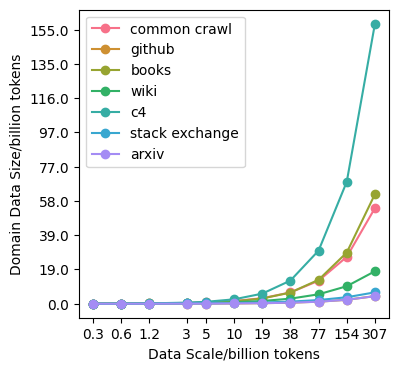
\includegraphics[width=\textwidth]{gptfigs/gptdata.png}
        \caption{\textsc{AutoScale}-predicted optimal data quantity for each domain as training data scales up.}
    \end{subfigure}
    % \hfill
    \hspace{1em}
    \begin{subfigure}[b]{0.51\textwidth}
        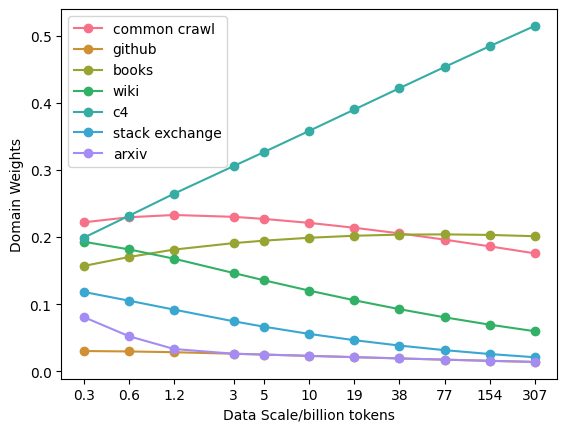
\includegraphics[width=\textwidth]{gptfigs/gptdmw.png}
        \caption{\textsc{AutoScale}-predicted optimal domain weights as training data scales up.}
    \end{subfigure}
    \caption{\textsc{AutoScale}-predicted domain weights for training 774M Decoder-only LMs. Optimal data quantity for each domain grows in exponential-style functions with training data scale (left) where data sources with diverse samples (e.g., \texttt{C4}) are upweighted relative to domains with standard format (e.g., \texttt{Wikipedia}).}\vspace{-0.5em}
    \label{fig:figure4}
\end{figure}

Fig.~\ref{fig:figure4} depicts \textsc{AutoScale}-predicted domain weights for training 774M Decoder-only LMs. Optimal data quantity for each domain grows in exponential-style functions with training data scale (left) where data sources with diverse samples (e.g., \texttt{C4}) are upweighted relative to domains with standard format (e.g., \texttt{Wikipedia}).

Fig.~\ref{fig:gpt2_additional_3} shows that when training on up to 5B tokens, \textsc{AutoScale}-predicted weights decreases val loss at least $25\%$ faster than any baseline with up to $37\%$ speed up. 

Fig.~\ref{fig:weights_gpt} visualizes domain weights used for training \texttt{GPT-2 Large}, given by different methods.

Table~\ref{tab:gpt2_additional_1} examines the domain-specific perplexity of \texttt{GPT-2 Large} trained on 3 billion tokens, respectively. Notably, \textsc{AutoScale} achieves the lowest average validation perplexity and significantly reduces the perplexity in the worst-performing domains.

Fig.~\ref{fig:doremi_ref_weights} visualizes \textsc{DoReMi} optimized domain weights with different reference weights and training steps. Training proxy/reference models for different steps gives different weights. It is unclear which weights are optimal. \textsc{DoReMi} recommends 200k steps, which equals >100B tokens in the default setup. Since optimization was conducted relative to the reference weights, reference weights have a profound impact on \textsc{DoReMi}'s output.


%######


\begin{table}[h!]\centering\resizebox{0.8\linewidth}{!}{
\begin{tabular}{l|c|ccc|c}
\toprule
\textbf{Domain/Method} & AutoScale            & DoReMi (Ref)        & Data Mixing    & LLaMA       & Uniform 
\\&&& Laws (ref) &&(30\% more tokens) \\ \midrule
Common Crawl           & 25.598           & \textbf{24.116} & 30.824          & 21.464  & 28.351                 \\
Github                 & 7.482           & 6.678          & \textbf{5.845} & 7.376  & 5.784                \\
Books                  & \textbf{29.162}  & 33.324          & 34.450          & 35.533  & 31.14                  \\
Wikipedia              & 18.828            & \textbf{17.154} & 26.795          & 21.110  & 19.57                  \\
C4                     & \textbf{34.242}  & 39.429          & 38.521          & 37.393  & 40.323                 \\
Stack Exchange         & 15.991           & 15.393          & \textbf{14.519} & 20.133  & 13.890                 \\
Arxiv                  & 16.558           & 15.638          & \textbf{12.372} & 17.598  & 13.082                 \\ \midrule
\textbf{Average}       & \textbf{21.123} & 21.676         & 23.333          & 22.944 & 21.736                \\ \midrule
\textbf{Worst-domain}  & \textbf{34.242} & 39.429         & 38.521         & 37.393 & 40.323                \\ \bottomrule
\end{tabular}}\vspace{1em}\caption{Domain perplexity for 774M Decoder-only LMs trained for 3B tokens. \textsc{AutoScale} notably achieves the lowest average validation perplexity while also significantly decreasing worse-domain perplexity.} \label{tab:gpt2_additional_1}
\end{table}





\begin{figure}[h!]
    \centering
    \begin{subfigure}[b]{0.48\textwidth}
        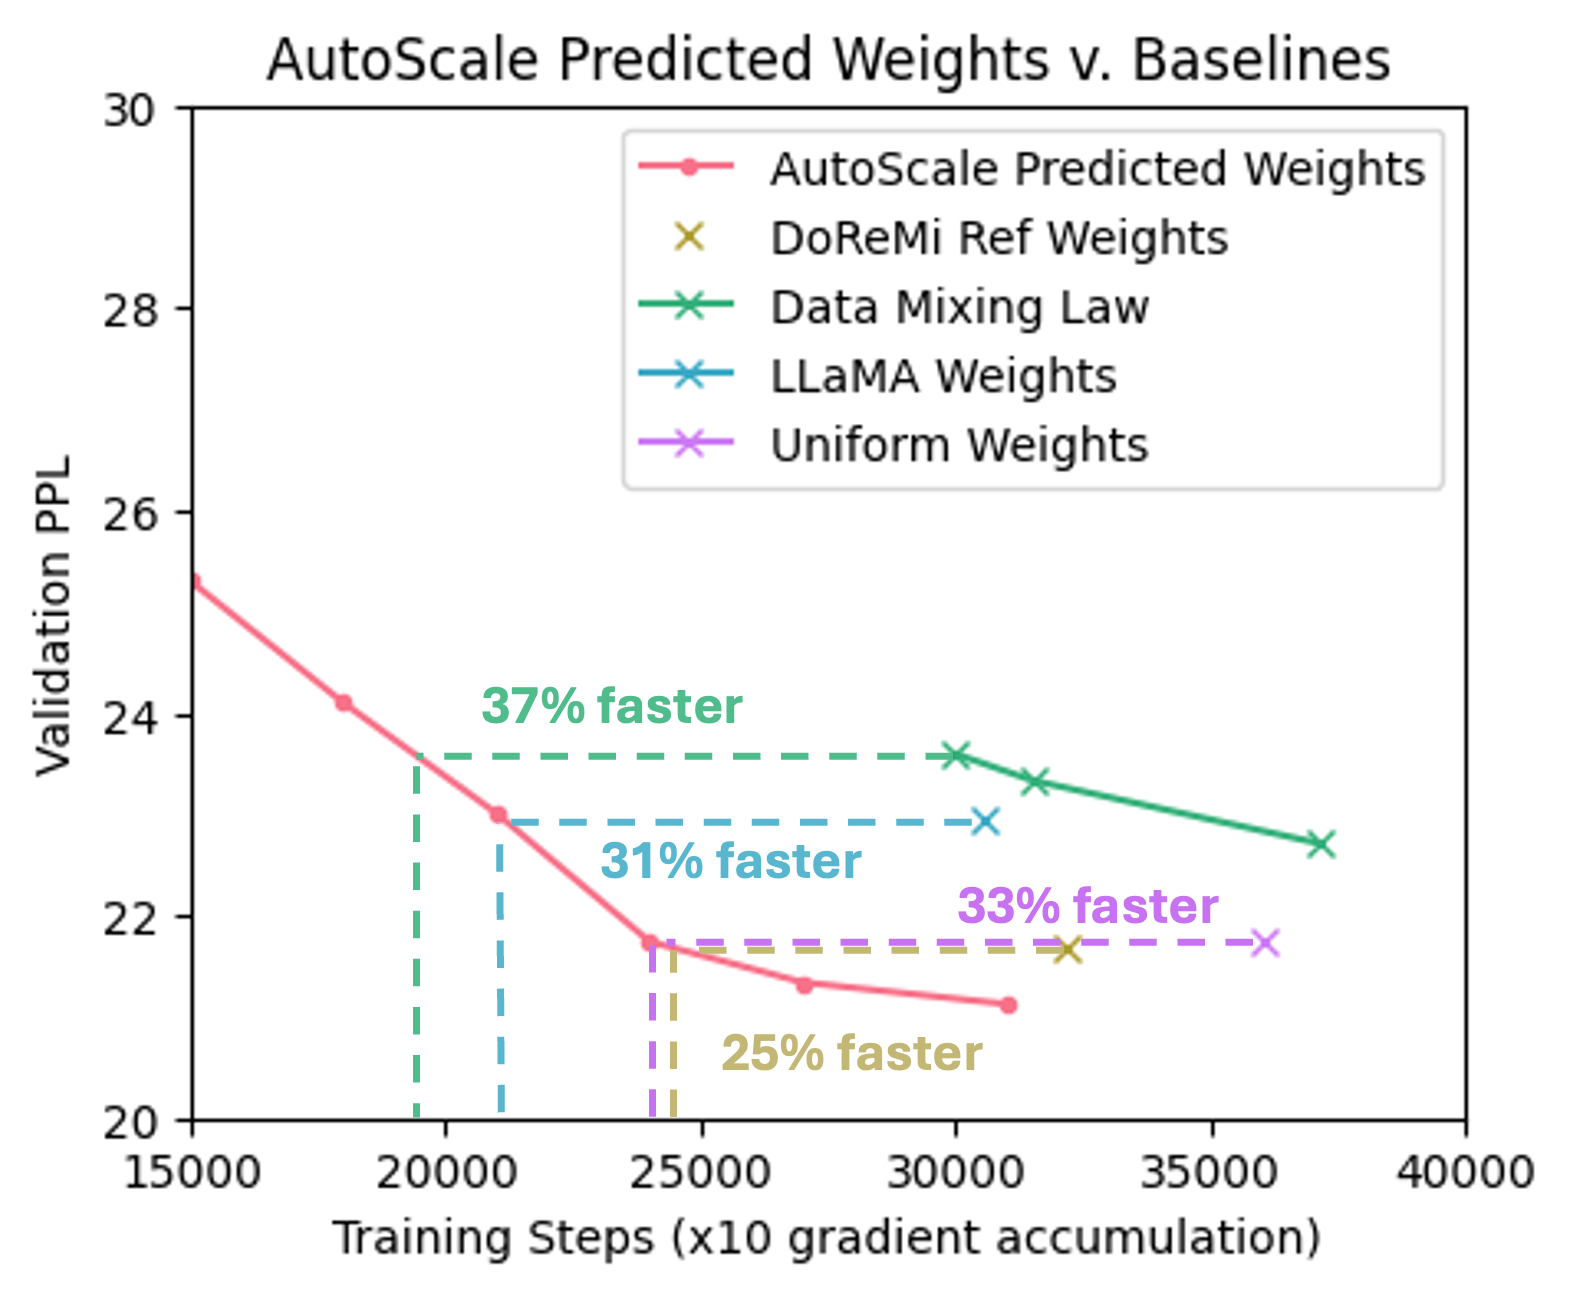
\includegraphics[width=\textwidth]{gptfigs/as500pr.png}
        \caption{Training Decoder-only LMs for 3B tokens.}
        \label{fig:figure7a}
    \end{subfigure}
    % \hfill
    % \hspace{1em}
    \begin{subfigure}[b]{0.48\textwidth}
        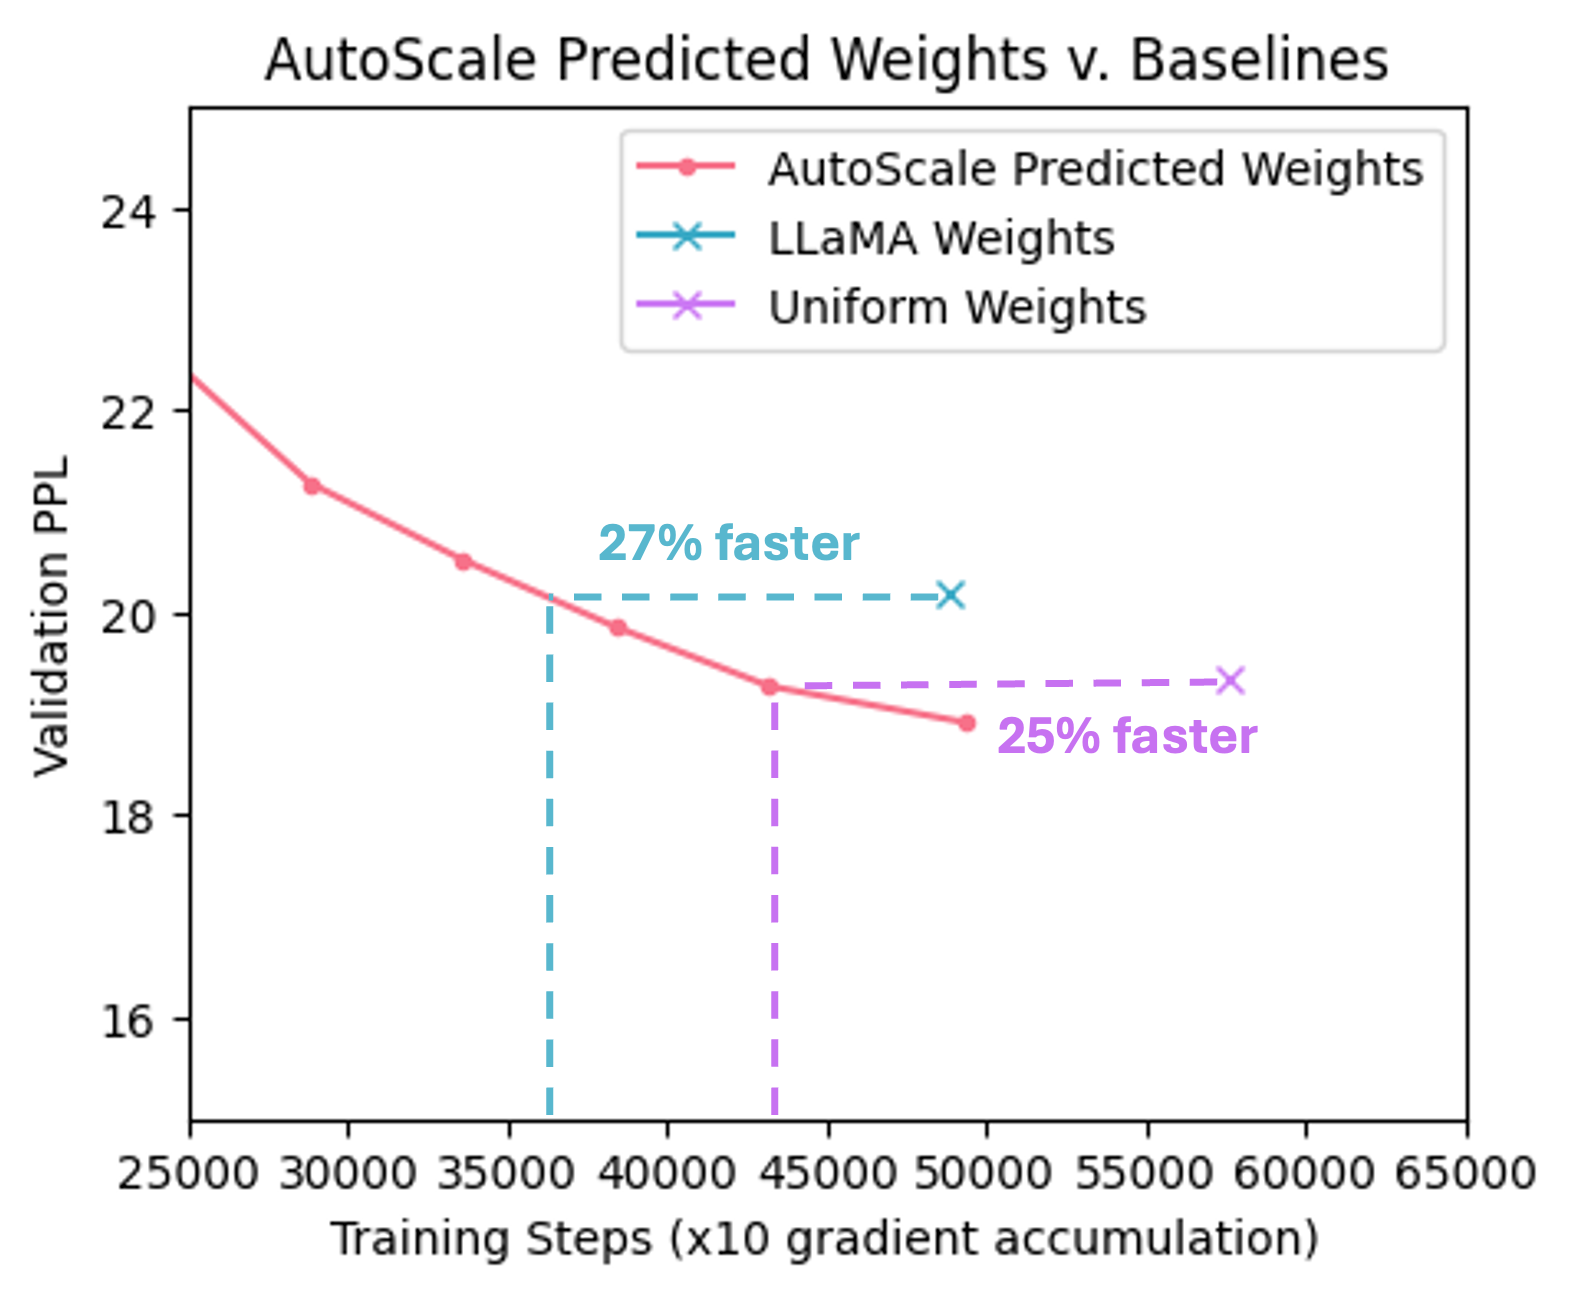
\includegraphics[width=\textwidth]{gptfigs/as800pr.png}
        \caption{Training Decoder-only LMs for 5B tokens.}
        \label{fig:figure7b}
    \end{subfigure}
    \caption{\textsc{AutoScale}-predicted weights decreases val loss at least $25\%$ faster than any baseline with up to $37\%$ speed up. Despite LLaMa weights being very different from uniform weights, they yield highly similar training efficiency at these data scales.}
    \label{fig:gpt2_additional_3}
\end{figure}

\begin{figure}[t!]
\begin{center}
  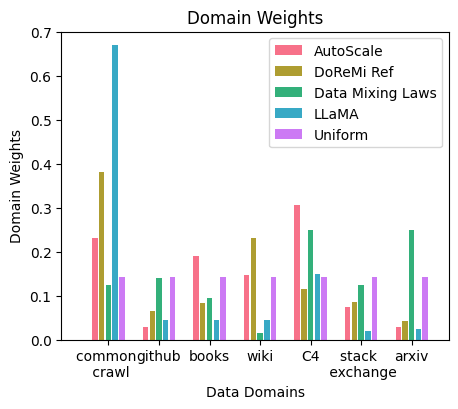
\includegraphics[width=0.5\textwidth]{gptfigs/dw500.png}
  \vspace{-1em}
  \caption{Domain Weights used for training 774M Decoder-only LMs for 3B tokens. (Domain weights for \textsc{Data Mixing Laws} and \textsc{DoReMi} are from references \citep{ye2024data} and \citep{fan2023doge}, respectively, which are implemented on the same datasets/data domains with highly similar model architecture/model size/tokenizers.)
  }\label{fig:weights_gpt}
  \vspace{-1em}
  \end{center}
\end{figure}% \vspace{-1em}



\begin{figure}[h!]
    \centering
    \begin{subfigure}[b]{0.45\textwidth}
        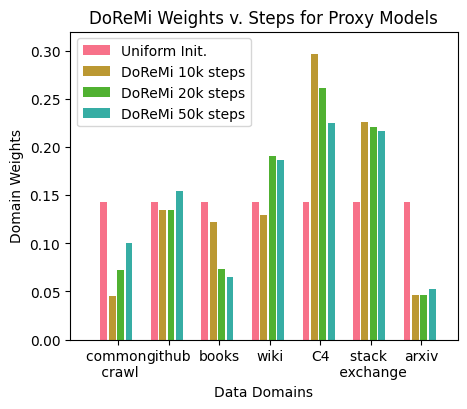
\includegraphics[width=\textwidth]{gptfigs/doremiUni.png}
        \caption{with Uniform Reference Weights}
    \end{subfigure}
    % \hfill
    \hspace{1em}
    \begin{subfigure}[b]{0.45\textwidth}
        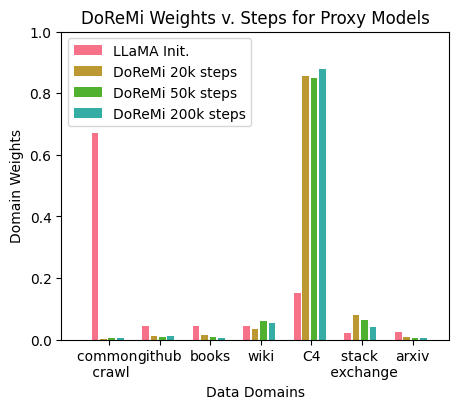
\includegraphics[width=\textwidth]{gptfigs/doremiLM.png}
        \caption{with LLaMA Reference Weights (Default)}
    \end{subfigure}
    \caption{\textsc{DoReMi} with different reference weights and steps.  Training proxy/reference models for different steps gives different weights. It is unclear which weights are optimal. \textsc{DoReMi} recommends 200k steps, which equals >100B tokens in the default setup. Since optimization was conducted relative to the reference weights, reference weights have a profound impact on \textsc{DoReMi}'s output.}
    \label{fig:doremi_ref_weights}
\end{figure}



\subsection{Additional Results of Sec.~\ref{sec:exp-bert}}
\label{sec:appendix_additional_results_bert}

Fig.~\ref{fig:figure30}(b) shows the results on fitting validation loss with power-law functions, directly approximating how loss changes with each domain's data quantity. Compared to \texttt{BERT} models trained with MLM (right), \texttt{GPT} models trained with CLM (left) demonstrate a much stronger response to domain reweighting. In final results, \texttt{GPT}/CLM achieved $> 2\times$ speed-up margins relative to uniform weights compared to \texttt{BERT}/MLM. 

Fig.~\ref{fig:bert_additional} depicts the \textsc{AutoScale}-predicted domain weights for training \texttt{BERT}. It is evident that optimal data quantity for each domain grows in exponential-style functions with training data scale where data sources with diverse samples (e.g., \texttt{WebText}) are upweighted relative to domains with standard format (e.g., \texttt{ArXiv}).

Table~\ref{table10} shows \textsc{AutoScale} notably improving training efficiency for \texttt{BERT} models on all scales–even for a considerably large scale, 288k steps, the speedup margin remains visible.

\begin{figure}[h!]
    \centering\vspace{-0.5em}
    \begin{subfigure}[b]{0.45\textwidth}
        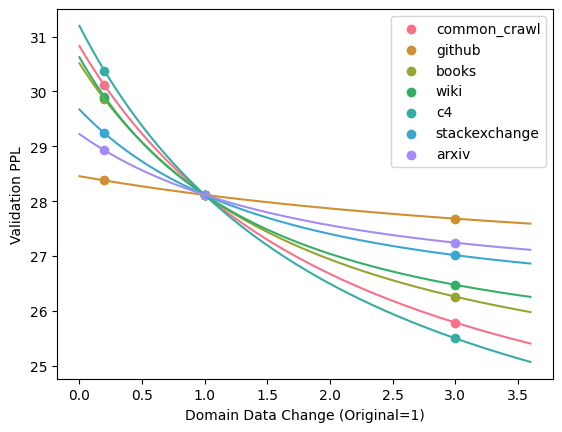
\includegraphics[width=\textwidth]{gptfigs/gptddo.png}
        \caption{774M Decoder-only LMs (\texttt{GPT-2 Large})}
    \end{subfigure}
    % \hfill
    \hspace{2em}
    \begin{subfigure}[b]{0.45\textwidth}
        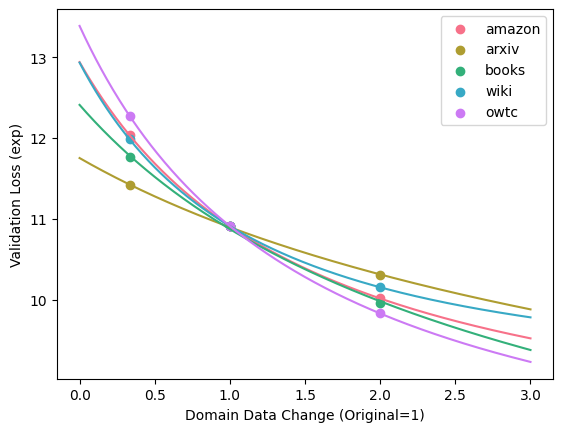
\includegraphics[width=\textwidth]{bertfigs/bertddo.png}
        \caption{Encoder-only LMs (\texttt{BERT-case})}
    \end{subfigure}
    \caption{Fitting validation loss with power-law functions, directly approximating how loss changes with each domain's data quantity. Compared to \texttt{BERT} models trained with MLM (right), \texttt{GPT} models trained with CLM (left) demonstrate a much stronger response to domain reweighting. In final results, \texttt{GPT}/CLM achieved $> 2\times$ speed-up margins relative to uniform weights compared to \texttt{BERT}/MLM. }
    \label{fig:figure30}\vspace{-1em}
\end{figure}

\begin{figure}[h!]
    \centering
    \begin{subfigure}[b]{0.4\textwidth}
        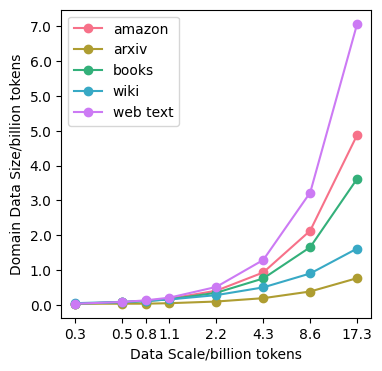
\includegraphics[width=\textwidth]{bertfigs/bertdata.png}
        \caption{\textsc{AutoScale}-predicted optimal data quantity for each domain as training data scales up.}
    \end{subfigure}
    % \hfill
    \hspace{1em}
    \begin{subfigure}[b]{0.51\textwidth}
        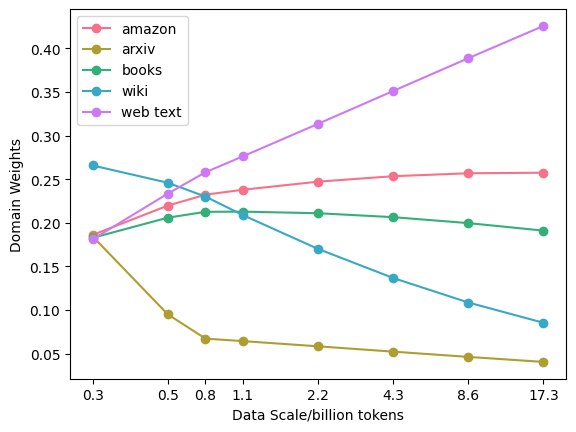
\includegraphics[width=\textwidth]{bertfigs/bertas.png}
        \caption{\textsc{AutoScale}-predicted optimal domain weights as training data scales up.}
        \label{fig:bert_additional_sub_2}
    \end{subfigure}
    \caption{\textsc{AutoScale}-predicted domain weights for training Encoder-only LMs (\texttt{BERT}). Optimal data quantity for each domain grows in exponential-style functions with training data scale (left) where data sources with diverse samples (e.g., \texttt{WebText}) are upweighted relative to domains with standard format (e.g., \texttt{ArXiv}).}
    \label{fig:bert_additional}
\end{figure}


\begin{table}[h!]\vspace{-0em}\centering{\resizebox{0.7\linewidth}{!}{
\begin{tabular}{lccccc}
\toprule
\textbf{Data Scale/steps} & 18k       & 36k       & 72k        & 144k       & 288k       \\\midrule
Final Loss (exp)  & 38.32     & 16.94     & 10.97      & 8.13       & 6.30       \\
Steps Saved       & 5k (28\%) & 5k (14\%) & 10k (14\%) & 20k (14\%) & 20k (10\%)\\
\bottomrule
\end{tabular}}}\caption{\textsc{AutoScale} notably improving training efficiency for \texttt{BERT} models on all scales–even for a considerably large scale, 288k steps, the speedup margin remains visible.}\label{table10}\vspace{-0.5em}
\end{table}

\subsection{Runtime Analysis}\label{runtime}
Training a \texttt{GPT-2 large} model from scratch for 3B tokens requires 15.5 hours on 8x NVIDIA A100 40GB SXM GPUs or 9 hours on 8x NVIDIA H100 80GB GPUs. Training time increases linearly with the number of training tokens on both types of GPUs.

Training \texttt{BERT-base} models takes 2 hours for every 18k steps on 4x NVIDIA A6000 48GB GPUs. Computational time grows linearly with the number of training steps.

Training reference models for \textsc{DoReMi} takes one hour for every 10K steps on 8x NVIDIA A6000 48GB GPUs. Computational time grows linearly with the number of training steps. Similar runtime for training proxy models for \textsc{DoReMi}. 


% \section{Discussions}

% Retraining-based gradient optimization is the most effective. Gradients must be calculated directly between the final objective (e.g., average exponential loss) and the optimization variable (data composition). Assuming data from each domain only/mostly affects its own performance leads to ineffective data selection.
% First-order gradient optimization needs to use line search to determine the optimal update at each step. The second-order gradient directly provides the optimal stepsize for each update.

% % \subsection{Connection to Curriculum Learning}

% \subsection{Reproducible \kang{rewrite}}


% The effect of noise must be carefully taken care of. Signal-to-noise ratio is a helpful tool for sanity checks. Some baseline papers produce false negative results for small signals overwhelmed by high noise.
\end{appendices}
% ============================================
% ============================================
% ============================================
% ============================================
% ============================================
% ============================================
% ============================================
% ============================================
% ============================================
% ============================================
% ============================================
% ============================================
% ============================================
% ============================================
% ============================================
% ============================================
% ============================================
% ============================================
% ============================================
% ============================================
% ============================================
% ============================================
% ============================================
% ============================================
% ============================================
% ============================================
% ============================================
% ============================================
% \newpage

% \section{Submission of papers to NeurIPS 2024}


% Please read the instructions below carefully and follow them faithfully.


% \subsection{Style}


% Papers to be submitted to NeurIPS 2024 must be prepared according to the
% instructions presented here. Papers may only be up to {\bf nine} pages long,
% including figures. Additional pages \emph{containing only acknowledgments and
% references} are allowed. Papers that exceed the page limit will not be
% reviewed, or in any other way considered for presentation at the conference.


% The margins in 2024 are the same as those in previous years.


% Authors are required to use the NeurIPS \LaTeX{} style files obtainable at the
% NeurIPS website as indicated below. Please make sure you use the current files
% and not previous versions. Tweaking the style files may be grounds for
% rejection.


% \subsection{Retrieval of style files}


% The style files for NeurIPS and other conference information are available on
% the website at
% \begin{center}
%   \url{http://www.neurips.cc/}
% \end{center}
% The file \verb+neurips_2024.pdf+ contains these instructions and illustrates the
% various formatting requirements your NeurIPS paper must satisfy.


% The only supported style file for NeurIPS 2024 is \verb+neurips_2024.sty+,
% rewritten for \LaTeXe{}.  \textbf{Previous style files for \LaTeX{} 2.09,
%   Microsoft Word, and RTF are no longer supported!}


% The \LaTeX{} style file contains three optional arguments: \verb+final+, which
% creates a camera-ready copy, \verb+preprint+, which creates a preprint for
% submission to, e.g., arXiv, and \verb+nonatbib+, which will not load the
% \verb+natbib+ package for you in case of package clash.


% \paragraph{Preprint option}
% If you wish to post a preprint of your work online, e.g., on arXiv, using the
% NeurIPS style, please use the \verb+preprint+ option. This will create a
% nonanonymized version of your work with the text ``Preprint. Work in progress.''
% in the footer. This version may be distributed as you see fit, as long as you do not say which conference it was submitted to. Please \textbf{do
%   not} use the \verb+final+ option, which should \textbf{only} be used for
% papers accepted to NeurIPS.


% At submission time, please omit the \verb+final+ and \verb+preprint+
% options. This will anonymize your submission and add line numbers to aid
% review. Please do \emph{not} refer to these line numbers in your paper as they
% will be removed during generation of camera-ready copies.


% The file \verb+neurips_2024.tex+ may be used as a ``shell'' for writing your
% paper. All you have to do is replace the author, title, abstract, and text of
% the paper with your own.


% The formatting instructions contained in these style files are summarized in
% Sec.~s \ref{gen_inst}, \ref{headings}, and \ref{others} below.


% \section{General formatting instructions}
% \label{gen_inst}


% The text must be confined within a rectangle 5.5~inches (33~picas) wide and
% 9~inches (54~picas) long. The left margin is 1.5~inch (9~picas).  Use 10~point
% type with a vertical spacing (leading) of 11~points.  Times New Roman is the
% preferred typeface throughout, and will be selected for you by default.
% Paragraphs are separated by \nicefrac{1}{2}~line space (5.5 points), with no
% indentation.


% The paper title should be 17~point, initial caps/lower case, bold, centered
% between two horizontal rules. The top rule should be 4~points thick and the
% bottom rule should be 1~point thick. Allow \nicefrac{1}{4}~inch space above and
% below the title to rules. All pages should start at 1~inch (6~picas) from the
% top of the page.


% For the final version, authors' names are set in boldface, and each name is
% centered above the corresponding address. The lead author's name is to be listed
% first (left-most), and the co-authors' names (if different address) are set to
% follow. If there is only one co-author, list both author and co-author side by
% side.


% Please pay special attention to the instructions in Sec.~\ref{others}
% regarding figures, tables, acknowledgments, and references.


% \section{Headings: first level}
% \label{headings}


% All headings should be lower case (except for first word and proper nouns),
% flush left, and bold.


% First-level headings should be in 12-point type.


% \subsection{Headings: second level}


% Second-level headings should be in 10-point type.


% \subsubsection{Headings: third level}


% Third-level headings should be in 10-point type.


% \paragraph{Paragraphs}


% There is also a \verb+\paragraph+ command available, which sets the heading in
% bold, flush left, and inline with the text, with the heading followed by 1\,em
% of space.


% \section{Citations, figures, tables, references}
% \label{others}


% These instructions apply to everyone.


% \subsection{Citations within the text}


% The \verb+natbib+ package will be loaded for you by default.  Citations may be
% author/year or numeric, as long as you maintain internal consistency.  As to the
% format of the references themselves, any style is acceptable as long as it is
% used consistently.


% The documentation for \verb+natbib+ may be found at
% \begin{center}
%   \url{http://mirrors.ctan.org/macros/latex/contrib/natbib/natnotes.pdf}
% \end{center}
% Of note is the command \verb+\citep+, which produces citations appropriate for
% use in inline text.  For example,
% \begin{verbatim}
%    \citep{hasselmo} investigated\dots
% \end{verbatim}
% produces
% \begin{quote}
%   Hasselmo, et al.\ (1995) investigated\dots
% \end{quote}


% If you wish to load the \verb+natbib+ package with options, you may add the
% following before loading the \verb+neurips_2024+ package:
% \begin{verbatim}
%    \PassOptionsToPackage{options}{natbib}
% \end{verbatim}


% If \verb+natbib+ clashes with another package you load, you can add the optional
% argument \verb+nonatbib+ when loading the style file:
% \begin{verbatim}
%    \usepackage[nonatbib]{neurips_2024}
% \end{verbatim}


% As submission is double blind, refer to your own published work in the third
% person. That is, use ``In the previous work of Jones et al.\ [4],'' not ``In our
% previous work [4].'' If you cite your other papers that are not widely available
% (e.g., a journal paper under review), use anonymous author names in the
% citation, e.g., an author of the form ``A.\ Anonymous'' and include a copy of the anonymized paper in the supplementary material.


% \subsection{Footnotes}


% Footnotes should be used sparingly.  If you do require a footnote, indicate
% footnotes with a number\footnote{Sample of the first footnote.} in the
% text. Place the footnotes at the bottom of the page on which they appear.
% Precede the footnote with a horizontal rule of 2~inches (12~picas).


% Note that footnotes are properly typeset \emph{after} punctuation
% marks.\footnote{As in this example.}


% \subsection{Fig.s}


% \begin{figure}
%   \centering
%   \fbox{\rule[-.5cm]{0cm}{4cm} \rule[-.5cm]{4cm}{0cm}}
%   \caption{Sample figure caption.}
% \end{figure}


% All artwork must be neat, clean, and legible. Lines should be dark enough for
% purposes of reproduction. The figure number and caption always appear after the
% figure. Place one line space before the figure caption and one line space after
% the figure. The figure caption should be lower case (except for first word and
% proper nouns); figures are numbered consecutively.


% You may use color figures.  However, it is best for the figure captions and the
% paper body to be legible if the paper is printed in either black/white or in
% color.


% \subsection{Tables}


% All tables must be centered, neat, clean and legible.  The table number and
% title always appear before the table.  See Table~\ref{sample-table}.


% Place one line space before the table title, one line space after the
% table title, and one line space after the table. The table title must
% be lower case (except for first word and proper nouns); tables are
% numbered consecutively.


% Note that publication-quality tables \emph{do not contain vertical rules.} We
% strongly suggest the use of the \verb+booktabs+ package, which allows for
% typesetting high-quality, professional tables:
% \begin{center}
%   \url{https://www.ctan.org/pkg/booktabs}
% \end{center}
% This package was used to typeset Table~\ref{sample-table}.


% \begin{table}
%   \caption{Sample table title}
%   \label{sample-table}
%   \centering
%   \begin{tabular}{lll}
%     \toprule
%     \multicolumn{2}{c}{Part}                   \\
%     \cmidrule(r){1-2}
%     Name     & Description     & Size ($\mu$m) \\
%     \midrule
%     Dendrite & Input terminal  & $\sim$100     \\
%     Axon     & Output terminal & $\sim$10      \\
%     Soma     & Cell body       & up to $10^6$  \\
%     \bottomrule
%   \end{tabular}
% \end{table}

% \subsection{Math}
% Note that display math in bare TeX commands will not create correct line numbers for submission. Please use LaTeX (or AMSTeX) commands for unnumbered display math. (You really shouldn't be using \$\$ anyway; see \url{https://tex.stackexchange.com/questions/503/why-is-preferable-to} and \url{https://tex.stackexchange.com/questions/40492/what-are-the-differences-between-align-equation-and-displaymath} for more information.)

% \subsection{Final instructions}

% Do not change any aspects of the formatting parameters in the style files.  In
% particular, do not modify the width or length of the rectangle the text should
% fit into, and do not change font sizes (except perhaps in the
% \textbf{References} section; see below). Please note that pages should be
% numbered.


% \section{Preparing PDF files}


% Please prepare submission files with paper size ``US Letter,'' and not, for
% example, ``A4.''


% Fonts were the main cause of problems in the past years. Your PDF file must only
% contain Type 1 or Embedded TrueType fonts. Here are a few instructions to
% achieve this.


% \begin{itemize}


% \item You should directly generate PDF files using \verb+pdflatex+.


% \item You can check which fonts a PDF files uses.  In Acrobat Reader, select the
%   menu Files$>$Document Properties$>$Fonts and select Show All Fonts. You can
%   also use the program \verb+pdffonts+ which comes with \verb+xpdf+ and is
%   available out-of-the-box on most Linux machines.


% \item \verb+xfig+ "patterned" shapes are implemented with bitmap fonts.  Use
%   "solid" shapes instead.


% \item The \verb+\bbold+ package almost always uses bitmap fonts.  You should use
%   the equivalent AMS Fonts:
% \begin{verbatim}
%    \usepackage{amsfonts}
% \end{verbatim}
% followed by, e.g., \verb+\mathbb{R}+, \verb+\mathbb{N}+, or \verb+\mathbb{C}+
% for $\mathbb{R}$, $\mathbb{N}$ or $\mathbb{C}$.  You can also use the following
% workaround for reals, natural and complex:
% \begin{verbatim}
%    \newcommand{\RR}{I\!\!R} %real numbers
%    \newcommand{\Nat}{I\!\!N} %natural numbers
%    \newcommand{\CC}{I\!\!\!\!C} %complex numbers
% \end{verbatim}
% Note that \verb+amsfonts+ is automatically loaded by the \verb+amssymb+ package.


% \end{itemize}


% If your file contains type 3 fonts or non embedded TrueType fonts, we will ask
% you to fix it.


% \subsection{Margins in \LaTeX{}}


% Most of the margin problems come from figures positioned by hand using
% \verb+\special+ or other commands. We suggest using the command
% \verb+\includegraphics+ from the \verb+graphicx+ package. Always specify the
% figure width as a multiple of the line width as in the example below:
% \begin{verbatim}
%    \usepackage[pdftex]{graphicx} ...
%    \includegraphics[width=0.8\linewidth]{myfile.pdf}
% \end{verbatim}
% See Sec.~4.4 in the graphics bundle documentation
% (\url{http://mirrors.ctan.org/macros/latex/required/graphics/grfguide.pdf})


% A number of width problems arise when \LaTeX{} cannot properly hyphenate a
% line. Please give LaTeX hyphenation hints using the \verb+\-+ command when
% necessary.

% \begin{ack}
% Use unnumbered first level headings for the acknowledgments. All acknowledgments
% go at the end of the paper before the list of references. Moreover, you are required to declare
% funding (financial activities supporting the submitted work) and competing interests (related financial activities outside the submitted work).
% More information about this disclosure can be found at: \url{https://neurips.cc/Conferences/2024/PaperInformation/FundingDisclosure}.


% Do {\bf not} include this section in the anonymized submission, only in the final paper. You can use the \texttt{ack} environment provided in the style file to automatically hide this section in the anonymized submission.
% \end{ack}

% \section*{References}


% References follow the acknowledgments in the camera-ready paper. Use unnumbered first-level heading for
% the references. Any choice of citation style is acceptable as long as you are
% consistent. It is permissible to reduce the font size to \verb+small+ (9 point)
% when listing the references.
% Note that the Reference section does not count towards the page limit.
% \medskip


% {
% \small


% [1] Alexander, J.A.\ \& Mozer, M.C.\ (1995) Template-based algorithms for
% connectionist rule extraction. In G.\ Tesauro, D.S.\ Touretzky and T.K.\ Leen
% (eds.), {\it Advances in Neural Information Processing Systems 7},
% pp.\ 609--616. Cambridge, MA: MIT Press.


% [2] Bower, J.M.\ \& Beeman, D.\ (1995) {\it The Book of GENESIS: Exploring
%   Realistic Neural Models with the GEneral NEural SImulation System.}  New York:
% TELOS/Springer--Verlag.


% [3] Hasselmo, M.E., Schnell, E.\ \& Barkai, E.\ (1995) Dynamics of learning and
% recall at excitatory recurrent synapses and cholinergic modulation in rat
% hippocampal region CA3. {\it Journal of Neuroscience} {\bf 15}(7):5249-5262.
% }


% %%%%%%%%%%%%%%%%%%%%%%%%%%%%%%%%%%%%%%%%%%%%%%%%%%%%%%%%%%%%

% \appendix

% \section{App.~/ supplemental material}


% Optionally include supplemental material (complete proofs, additional experiments and plots) in appendix.
% All such materials \textbf{SHOULD be included in the main submission.}

%%%%%%%%%%%%%%%%%%%%%%%%%%%%%%%%%%%%%%%%%%%%%%%%%%%%%%%%%%%%


\end{document}